%%% DOCUMENTCLASS 
%%%-------------------------------------------------------------------------------

\documentclass[
a4paper, % Stock and paper size.
11pt, % Type size.
% article,
% oneside, 
onecolumn, % Only one column of text on a page.
% openright, % Each chapter will start on a recto page.
% openleft, % Each chapter will start on a verso page.
openany, % A chapter may start on either a recto or verso page.
]{memoir}

%%% PACKAGES 
%%%------------------------------------------------------------------------------

\usepackage[utf8]{inputenc} % If utf8 encoding
% \usepackage[lantin1]{inputenc} % If not utf8 encoding, then this is probably the way to go
\usepackage[T1]{fontenc}    %
\usepackage[german]{babel} % German if it pleases m'lord
\usepackage[final]{microtype} % Less badboxes
\usepackage{csquotes} % For german quotations

% \usepackage{kpfonts} %Font

\usepackage{amsmath,amssymb,mathtools,polynom} % Math

% \usepackage{tikz} % Figures
\usepackage{graphicx} % Include figures

%%% PAGE LAYOUT 
%%%------------------------------------------------------------------------------

\setlrmarginsandblock{0.15\paperwidth}{*}{1} % Left and right margin
\setulmarginsandblock{0.2\paperwidth}{*}{1}  % Upper and lower margin
\checkandfixthelayout

%%% SECTIONAL DIVISIONS
%%%------------------------------------------------------------------------------

\maxsecnumdepth{subsection} % Subsections (and higher) are numbered
\setsecnumdepth{subsection}

\makeatletter %
\makechapterstyle{standard}{
  \setlength{\beforechapskip}{0\baselineskip}
  \setlength{\midchapskip}{1\baselineskip}
  \setlength{\afterchapskip}{8\baselineskip}
  \renewcommand{\chapterheadstart}{\vspace*{\beforechapskip}}
  \renewcommand{\chapnamefont}{\centering\normalfont\Large}
  \renewcommand{\printchaptername}{\chapnamefont \@chapapp}
  \renewcommand{\chapternamenum}{\space}
  \renewcommand{\chapnumfont}{\normalfont\Large}
  \renewcommand{\printchapternum}{\chapnumfont \thechapter}
  \renewcommand{\afterchapternum}{\par\nobreak\vskip \midchapskip}
  \renewcommand{\printchapternonum}{\vspace*{\midchapskip}\vspace*{5mm}}
  \renewcommand{\chaptitlefont}{\centering\bfseries\LARGE}
  \renewcommand{\printchaptertitle}[1]{\chaptitlefont ##1}
  \renewcommand{\afterchaptertitle}{\par\nobreak\vskip \afterchapskip}
}
\makeatother

\chapterstyle{standard}

\setsecheadstyle{\normalfont\large\bfseries}
\setsubsecheadstyle{\normalfont\normalsize\bfseries}
\setparaheadstyle{\normalfont\normalsize\bfseries}
\setparaindent{0pt}\setafterparaskip{0pt}

%%% FLOATS AND CAPTIONS
%%%------------------------------------------------------------------------------

\makeatletter                  % You do not need to write [htpb] all the time
\renewcommand\fps@figure{htbp} %
\renewcommand\fps@table{htbp}  %
\makeatother                   %

\captiondelim{\space } % A space between caption name and text
\captionnamefont{\small\bfseries} % Font of the caption name
\captiontitlefont{\small\normalfont} % Font of the caption text

\changecaptionwidth          % Change the width of the caption
\captionwidth{1\textwidth} %

%%% ABSTRACT
%%%------------------------------------------------------------------------------

\renewcommand{\abstractnamefont}{\normalfont\small\bfseries} % Font of abstract title
\setlength{\absleftindent}{0.1\textwidth} % Width of abstract
\setlength{\absrightindent}{\absleftindent}

%%% HEADER AND FOOTER 
%%%------------------------------------------------------------------------------

\makepagestyle{standard} % Make standard pagestyle

\makeatletter                 % Define standard pagestyle
\makeevenfoot{standard}{}{}{} %
\makeoddfoot{standard}{}{}{}  %
\makeevenhead{standard}{\bfseries\thepage\normalfont\qquad\small\leftmark}{}{}
\makeoddhead{standard}{}{}{\small\rightmark\qquad\bfseries\thepage}
% \makeheadrule{standard}{\textwidth}{\normalrulethickness}
\makeatother                  %

\makeatletter
\makepsmarks{standard}{
\createmark{chapter}{both}{shownumber}{\@chapapp\ }{ \quad }
\createmark{section}{right}{shownumber}{}{ \quad }
\createplainmark{toc}{both}{\contentsname}
\createplainmark{lof}{both}{\listfigurename}
\createplainmark{lot}{both}{\listtablename}
\createplainmark{bib}{both}{\bibname}
\createplainmark{index}{both}{\indexname}
\createplainmark{glossary}{both}{\glossaryname}
}
\makeatother                               %

\makepagestyle{chap} % Make new chapter pagestyle

\makeatletter
\makeevenfoot{chap}{}{\small\bfseries\thepage}{} % Define new chapter pagestyle
\makeoddfoot{chap}{}{\small\bfseries\thepage}{}  %
\makeevenhead{chap}{}{}{}   %
\makeoddhead{chap}{}{}{}    %
% \makeheadrule{chap}{\textwidth}{\normalrulethickness}
\makeatother

\nouppercaseheads
\pagestyle{standard}               % Choosing pagestyle and chapter pagestyle
\aliaspagestyle{chapter}{chap} %

%%% NEW COMMANDS
%%%------------------------------------------------------------------------------

% Polynomial long division
\polyset{%
	style=C,
	delims={\big(}{\big)},
	div=:
}

% Differential operator
\newcommand{\diff}[1]{\:\mathrm{d}{#1}}
\newcommand{\pdd}[2]{\frac{\partial #1}{\partial #2}}
\newcommand{\pddn}[3]{\frac{\partial^{#1} #2}{\partial #3^{#1}}}
\newcommand{\dd}[2]{\frac{\mathrm{d}{#1}}{\mathrm{d}{#2}}}
\newcommand{\ddn}[3]{\frac{\mathrm{d}^{#1}{#2}}{\mathrm{d}{#3^{#1}}}}

% N-th root
% \nroot{3}{27}
\newcommand*{\nroot}[2]{\sqrt[\leftroot{-1}\uproot{2}#1]{#2}}
\newcommand*{\ncroot}[4]{\sqrt[\leftroot{#1}\uproot{#2}#3]{#4}}

% 2 component vector
% \tvect{1}{-1}
% \tvec{1}{-1}
\newcommand{\tvect}[2]{%
   \ensuremath{\Bigl(\negthinspace\begin{smallmatrix}#1\\#2\end{smallmatrix}\Bigr)}}
\newcommand{\tvec}[2]{%
    \ensuremath{\left(\negthinspace\begin{matrix}#1\\#2\end{matrix}\right)}}

% 3 component vector
% \rvect{1}{-1}{0}
% \rvec{1}{-1}{0}
\newcommand{\rvect}[3]{%
   \ensuremath{\Bigl(\negthinspace\begin{smallmatrix}#1\\#2\\#3\end{smallmatrix}\Bigr)}}
\newcommand{\rvec}[3]{%
    \ensuremath{\left(\negthinspace\begin{matrix}#1\\#2\\#3\end{matrix}\right)}}

% Long vector arrow
% \xshlongvec{ABC}

% German-style quotation marks %
\MakeOuterQuote{"}

% Number sets
\newcommand{\N}{\mathbb{N}}
\newcommand{\Z}{\mathbb{Z}}
\newcommand{\Q}{\mathbb{Q}}
\newcommand{\R}{\mathbb{R}}
\newcommand{\C}{\mathbb{C}}

\newcommand{\setzero}{\varnothing}

% Mention (small caps)
\newcommand{\mention}[1]{\textsc{#1}}

% Functions
\newcommand{\asin}[0]{\text{asin}}
\newcommand{\acos}[0]{\text{acos}}
\newcommand{\atan}[0]{\text{atan}}
\newcommand{\sgn}[0]{\text{sgn}}
\newcommand{\grad}[0]{\text{grad}}

% Scale
% Usage in math mode: \Scale[1.5]{...equation...} %
\newcommand*{\Scale}[2][4]{\scalebox{#1}{$#2$}}%

% Units
\newcommand{\um}{\text{m}}
\newcommand{\us}{\text{s}}
\newcommand{\ukm}{\text{km}}
\newcommand{\ukg}{\text{kg}}
\newcommand{\uh}{\text{h}}
\newcommand{\ukmh}{\frac{\ukm}{\uh}}
\newcommand{\umpers}{\frac{\um}{\us}}
\newcommand{\umss}{\frac{\ukm}{\us^2}}
\newcommand{\ukgss}{\frac{\ukg}{\us^2}}
\newcommand{\degrees}[1]{\SI{#1}{\degree}}

% Floor / ceil
\newcommand{\floor}[1]{\left\lfloor #1 \right\rfloor}
\newcommand{\ceil}[1]{\left\lceil #1 \right\rceil}

% Circle characters
\newcommand*\circled[1]{
    \tikz[baseline=(char.base)]{
        \node[shape=circle,draw,inner sep=2pt] (char) {#1};
    }
}


%%%% NEW ENVIRONMENTS

\newenvironment{memo}
{\begin{quote}%
	\large\bfseries}
{\end{quote}}

%%%% NEW THEOREMS

\newtheorem{definition}{Definition}


%%% TABLE OF CONTENTS
%%%------------------------------------------------------------------------------

\maxtocdepth{subsection} % Only parts, chapters and sections in the table of contents
\settocdepth{subsection}

\AtEndDocument{\addtocontents{toc}{\par}} % Add a \par to the end of the TOC

%%% INTERNAL HYPERLINKS
%%%-------------------------------------------------------------------------------

\usepackage{hyperref}   % Internal hyperlinks
\hypersetup{
pdfborder={0 0 0},      % No borders around internal hyperlinks
pdfauthor={I am the Author} % author
}
\usepackage{memhfixc}   %


%%%% Named equations
%%%------------------------------------------------------------------------------
% Define Nequation environment for named equations.
% This is based on
%     http://tex.stackexchange.com/questions/128050/add-equation-name-underneath-equation-number
\usepackage{stackengine}
\def\stackalignment{r}
\def\stacktype{L}
\def\useanchorwidth{T}
% From page 3 of
%     http://tug.ctan.org/macros/latex/contrib/stackengine/stackengine.pdf
\def\Lstackgap{0.666666\baselineskip}
\newlength\eqshift
\setlength\eqshift{\widthof{)}}
\let\savetheequation\theequation
\newenvironment{Nequation}[1]%
{%
	\def\thecurrentname{#1}%
	\let\theequation\savetheequation
	\begin{equation}%
	\renewcommand\theequation
	{%
		\stackunder
		{\savetheequation}%
		{{\thecurrentname}\hspace{-\eqshift}}%
	}%
}%
{%
	\end{equation}%
	\addcontentsline{loe}{equation}{\protect\numberline{\theequation}\thecurrentname}%
	\let\theequation\savetheequation
	\ignorespacesafterend
}



\author{Andre Wachsmuth}

\title{Analysis / Infinitesimalrechnung}

\begin{document}

\frontmatter

\maketitle

\ifx\TEXPRINT\apar
\else
	\begin{center}
		\textbf{DRUCKVERSION}
	\end{center}
\fi

\begin{abstract}

Begleitende Notizen für die Modulvorlesung Analysis im Studiengang Informationstechnologie an der Berufsakademie Sachsen. Ziel ist die Einführung in die höhere Mathematik, speziell in die Theorie der Infinitesimalrechnung und Differenzgleichungen in Hinblick auf die Modellierung von physikalischen und anderen Sachverhalten. Es wird vorausgesetzt, dass grundlegende Kenntnisse aus der Mathematikausbildung der Seminarstufe I und II vorhanden sind.

\end{abstract}

\clearpage

\tableofcontents*

\clearpage

\chapter{Einführung}

\section{Organisatorisches}

\begin{itemize}
	\item Klausur: Schriftlich, 2 Stunden, davon $\frac{1}{3}$ Analysis, $\frac{2}{3}$ Algebra
	\item Hilfsmaterialen: Kein Taschenrechner, jeweils 1 handbeschriebenes A4-Blatt
	\item Online-Materialen: \href{https://drive.google.com/drive/folders/1CJ0226zg1_bnbt7IopCLwDuK2hkOgHya?usp=sharing}{drive.google.com}
	\item \LaTeX-Quellcode und weiteres: \href{https://github.com/blutorange/ba-dresden-calculus-awa}{github:blutorange/ba-dresden-calculus-awa}
	\item Kontakt: \href{mailto:wachsmuth.andre@gmx.de?subject=BA/Analysis 2020: }{wachsmuth.andre@gmx.de}
	\item Buchempfehlung: "Meyers kleine Enzyklopädie der Mathematik", hrsg. von Siegried Gottwald, Meyers Lexikonverlag, \href{https://www.amazon.de/-/en/Siegfried-Gottwald/dp/3411077719}{ISBN-3 3-411-07771-9}
	\item Buchempfehlung: "Repetitorium der höheren Mathematik", Merziger / Wirth, Binomi-Verlag, \href{https://www.amazon.de/-/en/Gerhard-Merziger/dp/3923923333}{ISBN-3 3-923-923-33-3}
    \item Buchempfehlung: "Ordinary Differential Equations", Tenenbaum / Pollard, \href{https://www.lehmanns.de/shop/mathematik-informatik/1860759-9780486649405-ordinary-differential-equations}{ISBN 978-0-486-64940-5}
\end{itemize}

\section{Anwendungen der Mathematik}

Mathematik stärkt die Fähigkeit zur Abstraktion und hilft bei der Lösung komplexer, auch nicht-mathematischer, Probleme. Grundlegend
ist die Fähigkeit, ein Problem analysieren zu können, es in Unterprobleme zu teilen und eine Lösungsstrategie zu erarbeiten zu können.

Auch in der Informatik und Programmierung sind mathematische Konzepte in einem breiten Umfang relevant.

\begin{itemize}
	\item In der objektorientierten Programmierung gibt es den Begriff der "Datenklassen". Um zu definieren, wie man diese vergleicht (\#equals) und ordnet (\#compareTo), werden Konzepte aus der Theorie der Relationen benötigt.
	\item Die Graphentheorie spielt eine wichtige Rollen bei Datenstrukturen und Algorithmen. Binäre Bäume stellen eine wichtige Datenstruktur für die effiziente Berechnung dar, gewichtete Graphen sind von wichtiger Bedeutung für das Problem des Handelsreisenden (Traveling Salesman), welches Anwendung findet in der Routenplanung, der Netzwerkarchitektur oder der Schaltkreisplanung.
	\item Grenzwertbetrachtungen und sogenannte Landau-Symbole werden genutzt, um die Laufzeit und den Speicherverbrauch von Algorithmen zu analysieren und zu beschreiben.
	\item Die Kategorientheorie ist eine Grundlage für algebraische Datenstrukturen. Zusammen mit dem $\lambda$-Kalkül stellen Sie die Basis funktionaler Programmierung dar.
	\item Die kontinuierliche Mathematik und die Infinitesimalrechnung stellen den Grundbaustein dar für physikalische Simulationen (Windtunnel, Crash-Test, Physics-Engine) und computergestützte Ingenieurswissenschaften (Gebäudestatik, Hydrodynamik, Schaltkreissimulation).
\end{itemize}

\section{Menge}

Selten betrachtet man nur eine konkrete Zahl, meist bespricht man von Mengen von Zahlen wie das Interval $[-3,3]$.  Als erstes benötigen wir eine genauere Vorstellung davon, was eine Menge ist.

\begin{definition}{Menge}{Set}
    Eine \textbf{Menge} ist eine Sammlung verschiedenartiger Elemente. Irrelevant hierbei ist die Reihenfolge der Elemente.
\end{definition}

Bei obiger Definition handelt es sich um den sogenannten naiven Mengenbegriff. Es hat sich gezeigt, dass diese naive Vorstellung zu Widersprüchen führen kann, weshalb präzisere Formulierungen der Mengentheorie gefunden wurden (etwa Zermelo–Fraenkel-Mengenlehre). Für diese Vorlesung ist der naive Mengenbegriff allerdings ausreichend.

Mengen kann man aus allen möglichen Elementen bilden. In dieser Vorlesung betrachten wir hauptsächlich Mengen aus Zahlen oder Vektoren. Für jeweils zwei Elemente solcher Mengen kann man einen Abstand definieren.

\begin{definition}{Norm}{Norm}
    Sei $M \subseteq \R^n$ eine Teilmenge von $n$-Tupeln reeller Zahlen (Punkte) und seien $x,y\in M$ zwei Punkte der Menge. Durch die Zuordnung
    $$
        m(x,y) = |x-y| = \sqrt{(x_1-y_1)^2 + \dots + (x_n-y_n)^2}
    $$
    wird eine \textbf{Norm} definiert, welche den Abstand oder die Distanz der beiden Punkte voneinander beschreibt.
\end{definition}

Damit lassen sich noch einige wichtige Arten von Mengen definieren:

\begin{definition}{Epsilon-Kugel um einen Punkt}{EpsilonSphere}
    Sei $x_0\in\R^n$ ein Punkt und $\epsilon > 0$. Dann heißt die Menge
    $$
        S_\epsilon(x_0) = \lbrace x \in M \hspace{3mm} | \hspace{3mm} |x-x_0| < \epsilon \rbrace
    $$
    eine (offene) \textbf{Epsilon-Kugel} um den Punkt $x_0$.
\end{definition}

\begin{definition}{Offene Menge}{OpenSet}
    Eine Teilmenge $M \subseteq \R^n$ der reellen Zahlen heißt \textbf{offene Menge}, wenn es für jeden Punkt der Menge eine Epsilon-Kugel gibt, die vollständig in der Menge liegt:
    $$
        \forall x \in M \exists \epsilon > 0: S_\epsilon(x) \subseteq M
    $$
\end{definition}

Anschaulich gesprochen hat eine offene Menge keinen Rand, siehe hierzu auch Abbildung \ref{fig:OpenClosedSet}.

\begin{definition}{Geschlossene Menge}{ClosedSet}
    Eine Teilmenge $M \subseteq \R^n$ der reellen Zahlen heißt \textbf{geschlossene Menge}, wenn ihr Komplement $\R^n \setminus M$ eine offene Menge ist.
\end{definition}

Anschaulich gesprochen unterscheiden sich eine offenen und eine geschlossene Menge nur dadurch, dass die geschlossene Menge einen Rand hat, der der offenen Menge fehlt.

\begin{definition}{Offene Umgebung eines Punktes}{OpenNeighborhood}
    Eine offene Menge $U(x) \subseteq \R^n$ heißt \textbf{offene Umgebung} des Punkts $x \in \R^n$ , wenn sie den Punkt $x$ enthält.
\end{definition}

\begin{figure}
    \centering
    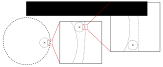
\includegraphics[width=0.55\textwidth]{./svg/open-set}
    
\includegraphics[width=0.35\textwidth]{./svg/closed-set}
    \caption{Definition einer offenen und geschlossenen Menge. Links: Zu jedem Elemente der Menge gibt es eine kleine Kugel, die vollständig in der Menge enthalten ist. Rechts: Die Grundgesamtheit ohne die geschlossene Menge ist ihrerseits eine offene Menge.}
    \label{fig:OpenClosedSet}
\end{figure}

\begin{figure}
    \centering
    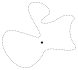
\includegraphics[width=0.3\textwidth]{./svg/open-neighborhood}
    \caption{Definitions der offenen Umgebung eines Punkts. Die Umgebung kann eine beliebige Form annehmen.}
    \label{fig:OpenNeighborhood}
\end{figure}

\section{Zahlenbereiche}

Grundlage für die gesamte Analysis die Objekte, auf denen sie operiert: Zahlen und Zahlenmengen. Zahlen modellieren quantitative Zusammenhänge der realen Welt. Gleichartige Zahlen abstrahiert man als eine Menge zu Zahlenbereichen.

Bei der Definition der Zahlenbereich beginnt man mit den natürlichen Zahlen und erweitert diese dann schrittweise.

\begin{definition}{Natürliche Zahlen}{NatNum}
	Die \textbf{natürlichen Zahlen} sind die Menge $\N$, die man erhält, wenn man mit dem Element $0$ beginnt und weitere Elemente rekursiv durch Bildung des Nachfolgers bestimmt.
\end{definition}

Präzisiert wird diese Definition durch die sogenannten \mention{Peano}-Axiome. Dabei kann man $0$ etwa mit dem Element $\setzero$ (leere Menge) identifzieren und die Nachfolgerbildung mit der Zuweisung
$\setzero \mapsto \lbrace \setzero \rbrace$ (Menge mit der leeren Menge). Der Vollständigkeit halber seien diese Axiome hier kurz angegeben.

\begin{definition}{\mention{Peano}-Axiome}{PeanoAx}
	\begin{enumerate}
		\item 0 ist eine Zahl.
		\item Jede Zahl $n$ hat genau einen Nachfolger $n'$.
		\item $0$ ist nicht Nachfolger einer Zahl.
		\item Jede Zahl ist Nachfolger höchstens einer Zahl.
		\item Von allen Mengen, die die Zahl $0$ und mit der Zahl $n$ auch deren Nachfolger $n'$ enthalten, ist die Menge $\N$ der natürlichen Zahlen diejenige mit den wenigsten Elementen.
	\end{enumerate}
\end{definition}

Natürliche Zahlen gibt es in zwei Ausprägungen. Die sogenannten \mention{Kardinalzahlen} beschreiben eine Anzahl, etwa die Anzahl von Büchern in einem Korb oder die Elemente in einem Array (Array-Länge).
Hinzu kommen die $\mention{Ordinalzahlen}$, welche eine Ordnung oder Rangfolge beschreiben. Im Gegensatz zu den Kardinalzahlen kann der Anfang bei Ordinalzahlen beliebig gewählt werden. Man kann den Index eines
Arrays sowohl bei $0$ als auch bei $1$ beginnen lassen, in beiden Fällen wird damit das \emph{erste} Element bezeichnet.

Nun reichen die natürlichen Zahlen nicht aus, um alle Gegebenheiten zu modellieren. Etwa ist es damit umständlich, Einnahmen und Kosten zu beschreiben. Hier müsste man immer angeben, ob es sich bei einer Quantität umd Einnahmen oder Kosten handelt und Regeln festlegen, wie Einnahmen und Kosten miteinander zu verrechnen sind. Um solche Gegensätze besser beschreiben zu können, führt man die ganzen Zahlen ein.
Kosten sind nun einfach beschreibbar als negative Einnahmen. Mathematisch motiviert werden die ganzen Zahlen, um ein inverses Element bezüglich der Addition angeben zu können. Dies wird unter dem Themengebiert siehe algebraische Strukturen im Modul Algebra näher beleuchtet.

\begin{definition}{Ganze Zahlen}{WholeNum}
	Die \textbf{ganzen Zahlen} sind die Menge $\Z$, die man aus $\N$ gewinnt, wenn man zu jeder natürlichen Zahl $n$ noch ihr Inverses $n'$ hinzunimmt. Dabei gilt $n+n' = n+(-n) = 0$.
\end{definition}

Doch auch die ganzen Zahlen sind unzureichend, um Verhältnisse und Verteilungen. Um etwa die Verteilung eines Geburtstagskuchen zu beschreiben, muss man immer die Grundgesamtheit (12 Stücke) als auch den Anteil
davon (3 Stück) angeben. Dies ist umständlich, stellt aber die Idee für die Definition der gebrochenen Zahlen dar.

\begin{definition}{Gebrochene Zahlen}{RatNum}
	Die \textbf{gebrochenen Zahlen} sind die Menge $\Q$, welche aus Paaren $(p,q) \in \Z^2$ ganzer Zahlen besteht. $p$ bezeichnet man dabei als Zähler, $q$ als Nenner. Zwei ganze Zahlen heißen äquivalent,  wenn
	diese den gleichen Bruch darstellen, also wenn gilt: $(p,q) \equiv (p',q') \iff pq'=p'q$
\end{definition}

Solche Brüche werden in der Informatik verwendet, um Fehler bei der Addition und Multiplikation zu vermeiden. Dies ist für einige Anwendungsbereiche wie Finanzen von wichtiger Bedeutung, um Geldbeträge
Cent-genau berechnen zu können. Ein Spezialfall davon ist die sogenannte Festkommazahlrechnung (fixed-point arithmetics), wobei der Nenner immer fest vorgeben ist.

Nun gibt es auch Rechenaufgaben, die selbst durch gebrochene Zahlen nicht gelöst werden können. Beispielsweise hat $x^2=2$ keine Lösung im Bereich der gebrochenen Zahlen. Allerdings ist es möglich,
Näherungswerte als Brüche anzugeben: $\frac{3}{2}, \frac{17}{12},\frac{577}{408}$. Man sieht hier, dass die Näherungswerte besser werden, also näher an der gesuchten Lösung liegen. Tatsächlich kann man
eine Formel angeben, um immer bessere Näherungswerte für $x^2=2$ zu finden. Alle diese Näherungswerte sind gebrochene Zahlen, dennoch gibt es keine gebrochene Zahl mit der Eigenschaft $x^2=2$.

\begin{definition}{Fundamentalfolge}{CauchySeq}
	Eine \textbf{Fundamentalfolge} (Cauchy-Folge) ist eine Zahlenfolge $a_i$, bei der der Abstand zweier Folgenglieder beliebig klein wird:

    \begin{equation}
        \forall \epsilon > 0: \exists N \in \N: \forall m,q>N: |a_m-a_q|<\epsilon
    \end{equation}
\end{definition}

Wie eben anhand des Beispiels $x^2=2$ illustriert, gibt es im Bereich der rationalen Zahlen Fundamentalfolgen, die sich zwar scheinbar einem Wert zu nähern scheinen (die also eine Cauchy-Folge darstellen),
wobei dieser Wert selber allerdings keine gebrochene Zahl ist. Zur Lösung dieses Problems werden die reellen Zahlen definiert.

\begin{definition}{Reelle Zahlen}{RealNum}
	Die \textbf{reellen Zahlen} sind die Menge $\R$, welche aus allen Fundamentalfolgen $a_i$ ganzer Zahlen besteht. Zwei Fundamentalfolgen $a_i, b_i$ sind dabei äquivalent, wenn $|a_i-b_i|$ eine Nullfolge bildet.
\end{definition}

Tatsächlich lässt sich zeigen, dass auf der Menge der reellen Zahlen $\R$ jede Cauchy-Folge konvergiert, also einen Grenzwert besitzt. Die reellen Zahlen sind im Gegensatz zu den gebrochenen Zahlen \emph{vollständig}.

Als Erweiterung der reellen Zahlen gibt es noch die komplexen Zahlen $\C$, wobei ein neues Element $j$ mit der Eigenschaft $j^2=-1$ eingeführt wird, welches die sogenannte imaginäre Einheit heißt. Komplexe
Zahlen eignen sich beispielsweise, um Schwingungen zu beschreiben oder Strom- und Spannungsberechnungen an Schaltkreisen anzustellen. Solche komplexen Zahlen werden in der Algebra genauer betrachtet. Diese Vorlesung beschränkt sich auf die reellwertige Analysis.

\section{Operationen und Rechenregeln}

Auf den Zahlenbereichen werden Rechenoperationen definiert, welche gewisse Regeln genügen. Die systematische Beschreibung solcher Rechenoperationen erfolgt durch das Gebiet algebraische Strukturen im Modul Algebra. Für die Analysis wird vorausgesetzt, dass elementare Rechenregeln aus Sekundarstufe I und II sowie der Umgang und die Umformung mathematischer Terme beherrscht werden. Im folgenden findet sich eine unvollständige Auflistung einiger wesentlicher Regeln:

\begin{statement}{Kommutativgesetz}{CommLaw}
	Für $a,b\in\R$ gilt: $a + b = b + a$
\end{statement}

\begin{statement}{Assoziativgesetz}{AssLaw}
	Für $a,b\in\R$ gilt: $a + ( b + c) = (a + b) + c$
\end{statement}

\begin{statement}{Distributivgesetz}{DisLaw}
	Für $a,b,c\in\R$ gilt: $a \cdot ( b + c ) = a \cdot b + a \cdot c$
\end{statement}

\begin{statement}{Potenzgesetze}{PowerIds}
	Für $x, y, p,q\in\R$, für welche die Potenzen erklärt sind, gelten die folgenden Rechenregeln:
	\begin{itemize}
		\item $x^{p+q} = x^p \cdot x^q$
		\item $x^p \cdot y^p = (x \cdot y)^p$
		\item $x^{(y^z)} = x^{y \cdot z}$
	\end{itemize}
\end{statement}

\begin{statement}{Logarithmengesetze}{LogIds}
	Für $x, y\in\R$, für welche die Logarithmen erklärt sind, gelten die folgenden Rechenregeln:
	\begin{itemize}
		\item $\ln(x \cdot y) = \ln(x) + \ln(y)$
		\item $\ln(x^y) = y \ln(x)$
		\item $\log_y(x) = \ln(x) / \ln(y)$
	\end{itemize}
\end{statement}

Für die Operationen $+$ (Addition) und $*$ (Multiplikation) gibt es zudem eine Kurzschreibweise, wenn eine (möglicherweise variable) Anzahl von Summanden addiert oder Faktoren multipliziert werden sollen. Man gibt dabei einen Laufindex an, der innerhalb gewisser Grenzen verläuft, und einen Term, in den jeder erlaubte Wert des Laufindex eingesetzt wird. Die Werte des Terms für jeden Laufindex werden dann addiert beziehungsweise multipliziert. Geschrieben wird dies wie folgt:

$$
\sum\limits_{i=1}^{10} i^2  \\
$$

$$
\prod\limits_{i=1}^{5} i
$$

Oben steht eine Summe ($\Sigma$ für Sigma, Summe), gesprochen: "Die Summe von i gleich 1 bis 10 über i-Quadrat." Es sollen also die ersten 10 Quadratzahlen addiert werden. Unten steht ein Produkt ($\Pi$ für Pi, Produkt), gesprochen: "Das Produkt von i gleich 1 bis 5 über i." Hier sollen also die Zahlen von $1$ bis $5$ multipliziert werden ($=5!$). Man beachte auch die Analogie zu einer \emph{For-Schleife} in der Programmierung:

\begin{jscode}
sum = 0;
for (i = 1; i <= 10; ++i)
	sum += i * i;
\end{jscode}

\section{Schlussfolgern}

Ein in der Schulmathematik häufig vernachlässigter wichtiger Bestandteil der Mathematik ist das Schlussfolgern, also dem Ziehen von Schlüssen basierend auf gewissen Grundannahmen oder Axiomen. Hierfür
gibt es einige wichtige Techniken wie \emph{Induktion} oder \emph{reductio ad absurdum}. Auch wenn das Beweisführen in dieser Vorlesung nicht im Vordergrund steht, wird erwartet, dass zu einer Antwort
immer eine knappe, aber fundierte Begründung (Rechenweg oder Prosa) gegeben wird. In folgenden wird anhand einiger Beispiele kurz illustriert, wie mathematische Beweise geführt werden können.

\subsection{Beweis durch Widerspruch}

Frage: Ist $\sqrt{2}\in\Q$?

Wir nehmen an, $\sqrt{2}$ wäre eine gebrochene Zahl, also darstellbar als vollständig gekürzter Bruch $\frac{p}{q}, p,q\in\Z, p,q>0$. Dann sind $p$ und $q$ teilerfremd. Es folgt nun:

\begin{align}
  \sqrt{2} & = p / q \\
         2 & = p^2 / q^2 \\
     2 q^2 & = p^2 \label{eq:sqrt2-p2even}
\end{align}

Aus Gleichung \ref{eq:sqrt2-p2even} folgt, $p^2$ ist eine gerade Zahl, da es sich als das doppelte einer anderen ganzen Zahl $q^2$ darstellen lässt. Weiterhin ist damit auch $p$ eine gerade Zahl, da das Produkt zweiter ungerade Zahlen
immer ebenfalls eine ungerade Zahl ergibt. Wir können $p$ nun schreiben als $p = 2 n, n\in \Z$. Es ergibt sich:

\begin{align}
	2q^2 & = p^2 = p * p = (2n) \cdot (2n) \\
	q^2 & = 2 n^2 \label{eq:sqrt2-q2even}
\end{align}

Da $n$ eine ganze Zahl ist, so ist auch $n^2$ eine ganze Zahl. Wegen \ref{eq:sqrt2-q2even} lässt sich $q^2$ sich schreiben als das doppelte einer ganzen Zahl und ist daher eine gerade Zahl, mithin ist also auch $q$ eine gerade Zahl.

Nun haben wir damit aber gezeigt, dass sowohl $p$ als auch $q$ gerade Zahlen sind. Sie besitzen also beide den Teiler $2$. Dies widerspricht der Annahme, dass es einen vollständig gekürzten Bruch $p / q = \sqrt{2}$ gibt. Die Annahme, dass es einen solchen Bruch gibt, wurde damit zu einem Widerspruch (ad absurdum) geführt (reductio). Somit gibt es keine gebrochene Zahl $x$ mit der Eigenschaft $x^2=2$.

\subsection{Nichtkonstruktiver Beweis}

Frage: Gibt es zwei irrationale Zahlen $x,y\notin \Q$ so, dass deren Potenz $x^y\in \Q$ eine rationale Zahl ergibt?

Wir wählen $x=y=\sqrt{2}$. Nach dem Satz vom ausgeschlossenen Dritten ist eine Aussage entweder wahr oder falsch, das heißt entweder gilt $\sqrt{2}^{\sqrt{2}} \in \Q$ oder $\sqrt{2}^{\sqrt{2}}\notin\Q$. Wir betrachten beide Fälle:

\begin{itemize}
	\item $\sqrt{2}^{\sqrt{2}}\in\Q$: $\sqrt{2}$ ist wie eben gezeigt irrational, damit ist ein Beispiel für zwei solche Zahlen gefunden.

	\item $\sqrt{2}^{\sqrt{2}}\notin\Q$: Wir setzen $x' = \sqrt{2}^{\sqrt{2}}$ und $y'=\sqrt{2}$. Die Zahl $x'$ ist nach Annahme irrational und die Potenz $(\sqrt{2}^{\sqrt{2})^{\sqrt{2}}} = \sqrt{2}^{\sqrt{2}\sqrt{2}} = \sqrt{2}^2 = 2$ ist eine rationale Zahl.
\end{itemize}

Wir haben damit gezeigt, dass es wenigstens eine Paar zwei solcher Zahlen gibt, nämlich entweder $(x,y) = (\sqrt{2}, \sqrt{2})$ oder $(x,y) = (\sqrt{2}^{\sqrt{2}}, \sqrt{2})$. Dieser Beweis heißt deshalb nichtkonstruktiv, da er keine Möglichkeit bietet, zu bestimmen, welche Zahlen es tatsächlich sind.

\section{Struktur von Termen}

Um mathematische Ideen zu kommunizieren, ist eine Notation notwendig, die gewissen Regeln folgt. Um etwa die Idee zu beschreiben, dass die Summe zweier Zahlen in einer Menge enthalten sei, wird in der üblichen mathematischen Notation die Schreibweise $a+b\in\N$ verwendet. Wir an diesem Beispiel zu sehen, besteht die mathematische Notation also zum Einen aus Symbolen für mathematische Objekte und Operationen und zum Zweiten aus Regeln, wie diese Symbole angeordnet werden dürfen. Genau dies ist aber die Definition einer sogenannten \emph{formalen Sprache} mit Wörtern und einer Grammatik für die Bildung von Sätzen.

Man beachte die Analogie zu Programmiersprachen, auch diese stellen eine solche formale Sprache dar. Genauso wie ein Programm dargestellt werden kann als \emph{Syntaxbaum} ist dies auch mit einem mathematischen Ausdruck möglich. Ein Syntaxbaum beginnt immer an der Spitze mit der hauptsächlichen Operation, und verzweigt dann in die einzelnen Unteroperation. Wir betrachten als Beispiel zuerst das folgende Computerprogramm zur Berechnung der $n$.-ten Fibonacci-Zahl in Listing \ref{lst:JsFibonacci}.

\begin{listing}
\begin{jscode}
function fibonacci(n) {
	let n_0 = 0;
	let n_1 = 1;
	while (n-- > 0) {
		const sum = n_0 + n_1;
		n_0 = n_1;
		n_1 = sum;
	}
	return n_0;
}
\end{jscode}
\caption{JavaScript-Programm zur Berechnung der n.-ten Fibonacci-Zahl}
\label{lst:JsFibonacci}
\end{listing}


In oberster Ebene ist die Struktur dieses Programms eine \emph{Function Declaration}, bestehend aus einem Funktionsnamen, einem Argument und einem Funktionskörper. Der Funktionskörper selbst ist zuallererst ein \emph{Block Statement}, bestehend aus einer \emph{Statement List}. Das Statement auf Zeile 5, \lstinline{const sum = n_0 + n_1}, wiederum ist ein \emph{Variable Declaration}-Statement, bestehend aus einem \emph{Identifier} für den Variablennamen und einem \emph{Initializer} für den Wert der Variablen. Der \emph{Initializer} ist eine \emph{Sum Expression} (Summen-Ausdruck), der wiederum aus 2 Summanden besteht. Jeder Summand ist in diesem Fall ein \emph{Identifier} für den jeweiligen Variablennamen. Verbal formuliert mag diese Struktur nur schwer vorstellbar sein. Graphisch ist der Syntaxbaum auszugsweise in Abbildung \ref{fig:JsFibonacciBaumPart} dargestellt. Der vollständige Syntaxbaum findet sich in Abbildung \ref{fig:JsFibonacciBaum}.

\begin{figure}
	\centering
	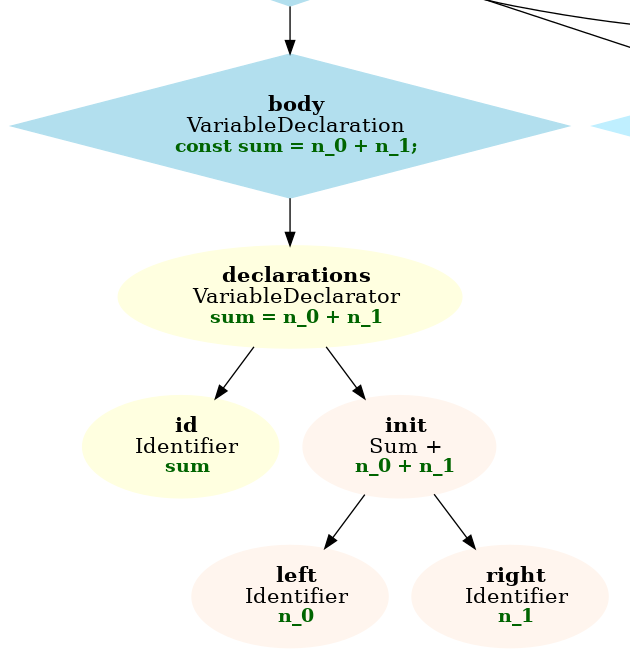
\includegraphics[width=0.5\textwidth]{./img/js-tree-fibonacci-part.png}
	\caption{Syntaxbaum zum JavaScript-Programm für Fibonacci-Zahlen (Auszug)}
	\label{fig:JsFibonacciBaumPart}
\end{figure}

Für die mathematische Notation besonders relevant sind die Ausdrücke (\emph{Expression}), also Rechenoperationen. Einen mathematischer Term lässt wie erwähnt als Syntaxbaum darstellen. Solch ein Syntaxbaum lässt sich schriftlich auf verschiedene Weisen schreiben. Die mathematische Notation lehnt sich an der sogenannten Infix-Notation an, wobei die Operatoren zwischen die Operanden geschrieben werden. Eine weitere Notation stellt die Polnische Notation dar, die etwa in manchen Taschenrechner verwendet wird und auch die Grundlage für \mention{Ldap}-Filter darstellt (Lightweight Directory Access Protocol). Wir wollen dies kurz am Beispiel $(a+b)\cdot(c+d)$ illustrieren. Der Syntaxbaum dazu ist zu finden in Abbildung \ref{fig:JsAbcdBaum}.

\begin{figure}
	\centering
	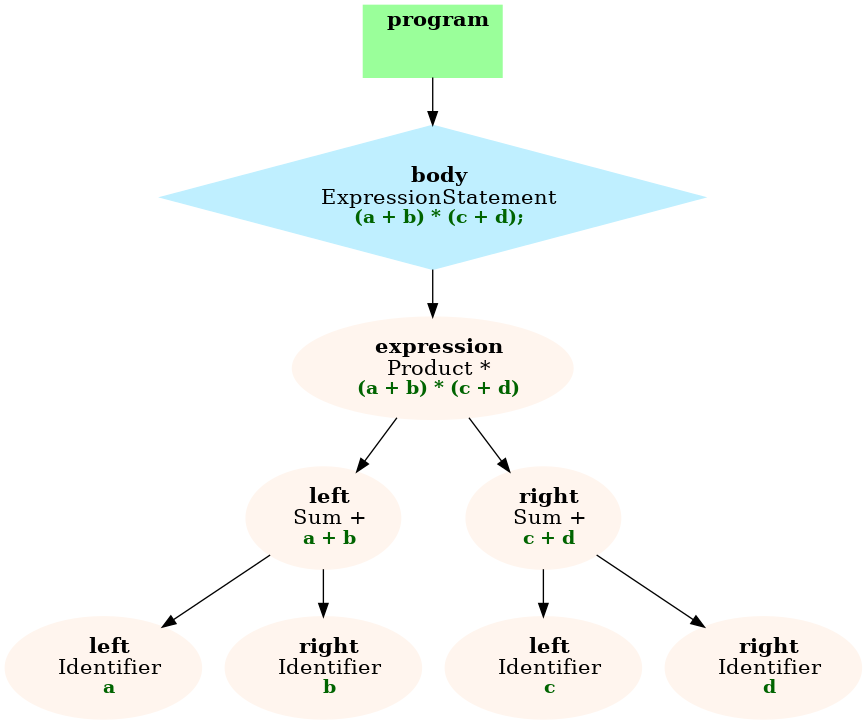
\includegraphics[width=0.5\textwidth]{./img/js-tree-abcd.png}
	\caption{Syntaxbaum für $(a+b)(c+d)$}
	\label{fig:JsAbcdBaum}
\end{figure}

Aus dem Syntaxbaum lesen wir ab, dass der Term aus der Hauptoperation \emph{Multiplikation} besteht. Die beiden Faktoren bestehen jeweils aus einer Unteroperation, hier einen Summenbildung. Die Infix-Notation $(a+b)\cdot(c+d)$ beginnt daher mit einem Multiplikationszeichen, zu dessen beiden Seiten Summenzeichen stehen. Um die Rangfolge zu wahren, welche durch den Syntaxbaum vorgegeben ist, erfordert die Infix-Notation die Verwendung von Klammerzeichen. Eine Alternative zur Infix-Notation ist die polnische Notation, welche keine Klammerzeichen benutzt und so etwa einfacher von Computerprogramme verstanden werden kann. Dies erreicht sie dadurch, indem sie zuerst für jeden Operator definiert, welche Arität (Anzahl von Operanden) er hat. Anschließend wird der Operator nicht zwischen die Operanden, sondern vor die Operanden geschrieben. Zusätzlich gibt es noch die sogenannte umgekehrte polnische Notation, wobei der Operator nicht vor, sondern nach den Operanden notiert wird. Für unser Beispiel $(a+b)(c+d)$ ist die polnische Notation dargestellt in Listing \ref{lst:PolAbcd}.

\begin{listing}
\begin{textcode}
* + a b + c d
a b + c d + *
\end{textcode}
	\caption{Polnische Notation (oben) und umgekehrte polnische Notation (unten)}
	\label{lst:PolAbcd}
\end{listing}

Schließlich sei noch angemerkt, dass Rechenregeln sich darstellen lassen als Transformationen auf einem Syntaxbaum. Dies stellt die Grundlage dar für Computer-Algebra-System, welche auf symbolischen Ausdrücken arbeiten und diese umformen können. Dies ist in Abbildung \ref{fig:TreeTransformKommutativ} am Beispiel des Kommutativgesetzes dargestellt. Dieses besagt, dass bei einer \emph{Sum Expression} die beiden Unterbäume der beiden Summanden vertauscht werden können. Man beachte, dass die Summanden im Allgemeinen nicht Zahlen oder Variablen, sondern wiederum komplexe Baumstrukturen sind.

\begin{figure}
	\centering
	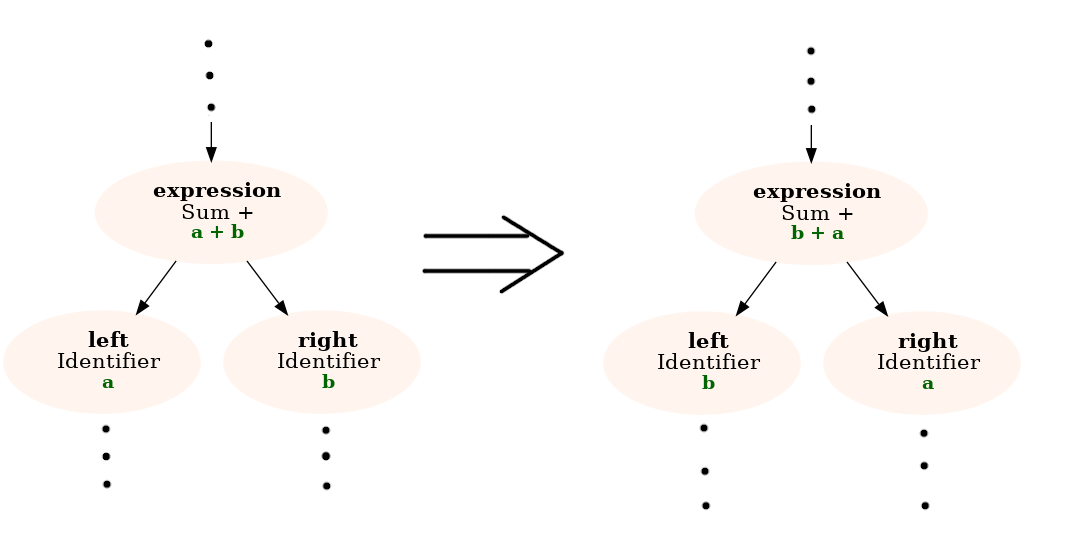
\includegraphics[width=0.8\textwidth]{./img/tree-transform.png}
	\caption{Syntaxbaumtransformation für das Kommutativgesetz}
	\label{fig:TreeTransformKommutativ}
\end{figure}

\mainmatter

% Sequences, sums, limit (definition), convergence criteria
\chapter{Zahlenfolgen, Zahlenreihen, Konvergenz}

Der moderne Grenzwertbegriff stellt die Grundlage der Infinitesimalrechnung dar. In diesem Kapitel betrachten wir zuerst Zahlenfolgen und Reihen, definieren dann Konvergenz sowie Grenzwert und lernen abschließend einige wichtige Regeln zur Konvergenz und Grenzwertbestimmung kennen.

Um die Wichtigkeit zu illustrieren, warum eine exakte Definition der Konvergenz notwendig ist, sei Zenons Paradoxon von Achilles und der Schildkröte angeführt. \emph{Zeno of Elea} (etwa 500 BC) hat dieses Paradoxon angeführt, um zu zeigen, dass der naive Begriff von Wandel und Bewegung nur eine Illusion wäre. Zur besseren Veranschaulichung wählen für die folgende Erklärung (willkürlich gewählte) Größenabgaben. In dem Paradox nun veranstalten Achilles und eine Schildkröte ein Wettrennen, wie in Abbildung \ref{fig:ZenoAchilles} dargestellt. Achilles ist in der Lage, mit einer Geschwindigkeit von $25\ukmh$ zu rennen, während die Schildkröte nur $5\ukmh$ schafft. Der Fairness halber erhält die Schildkröte daher einen Vorsprung von $100\ukm$. Die Frage ist nun, wann Achilles die Schildkröte überholt. Der geläufige physikalische Ansatz wäre, ein Koordinatensystem zu definieren, die Bewegungsgleichungen beider Partizipanten aufzustellen und den Schnittpunkt zu berechnen. Zenon argumentiert allerdings wie folgt:

\begin{enumerate}
	\item Damit Achilles die Schildkröte überholen kann, muss er zunächst den Vorsprung von $100\ukm$ aufholen. Dazu benötigt er $4$ Stunden.
	\item In diesen $4$ Stunden allerdings ist die Schildkröte bereits $20\ukm$ weiter gekrochen.
	\item Also muss Achilles im nächsten Schritt diese $20\ukm$ Vorsprung aufholen, wozu er $0.8$ Stunden benötigt. Aber nun hat die Schildkröte bereits einen neuen Vorsprung erhalten.
	\item Egal, wie oft Achilles also den Vorsprung aufholt, um die Schildkröte zu überholen, müsste er unendliche viele Vorsprünge aufholen. Also holt Achilles die Schildkröte nie ein, um kann sie somit auch nicht überholen.
\end{enumerate}

Wie lässt sich dieses Paradoxon auflösen? Der Fehler, den Zenon hier begeht, besteht darin, dass Achilles zum Aufholen "unendlich" vieler Vorsprünge auch "unendlich" viel Zeit benötigt. Dies ist aber bei einer genauen Betrachtung mithilfe eines exakten Grenzwertbegriffs nicht der Fall, wie wir auch in einer Übungsaufgabe nachweisen werden.

\begin{figure}
	\centering
	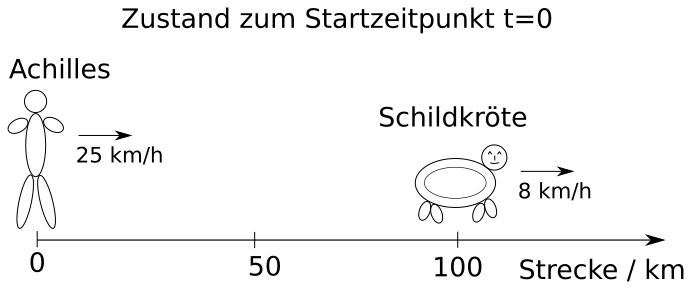
\includegraphics[width=0.75\textwidth]{./svg/zeno-achilles.png}
	\caption{Zenos Paradoxon von dem Wettrennen zwischen Achilles und der Schildkröte}
	\label{fig:ZenoAchilles}
\end{figure}

\section{Zahlenfolgen}

Bevor wir den Begriff der Konvergenz näher definieren können, benötigen wir zuerst ein Verständnis von Zahlenfolgen.

\begin{definition}{Unendliche Zahlenfolge}{UnlimitSeq}
	Eine unendliche Zahlenfolge ist gegeben, wenn jeder natürlichen Zahl $n \ge 0$  genau eine (meist reelle) Zahl $a_n\in\R$ zugeordnet wird. $a_n$ heißt das $(n+1)$-te Glied der Zahlenfolge.
\end{definition}

\begin{definition}{Endliche Zahlenfolge}{LimitSeq}
	Besteht die Zuordnung nur für jede natürliche Zahl $n$ zwischen 0 und $N$ ($0 \ge n \ge N$), so spricht man von einer endlichen Zahlenfolge.
\end{definition}

Zahlenfolgen können also als Funktion $f: \N \to \R$ aufgefasst werden. Zur mathematischen Darstellung gibt es zwei Möglichkeiten:

\begin{enumerate}
	\item Explizite Darstellung: Der Wert des $n$.-ten Folgenglieds ist direkt gegeben.
	\item Implizite (rekursive) Darstellung: Der Wert des nächsten Folgengliedes ($n+1$) ist gegeben in Abhängigkeit eines oder mehrerer voriger Folgenglieder. Zudem ist ein Startwert für das erste oder die ersten Folgenglieder gegeben.
\end{enumerate}

Wir wollen uns diese beiden Möglichkeiten an zwei wichtigen Zahlenfolgen anschauen.

\begin{definition}{Arithmetische Zahlenfolge}{ArithSeq}
	Eine arithmetische Zahlenfolge ist gegeben, wenn in jedem Schritt das nächste Folgenglied durch Addition einer immer gleichen Konstanten zum vorigen Folgenglied bestimmt wird.
\end{definition}

\begin{definition}{Geometrische Zahlenfolge}{GeoSeq}
	Eine geometrische Zahlenfolge ist gegeben, wenn in jedem Schritt das nächste Folgenglied durch Multiplikation einer immer gleichen Konstanten mit dem vorigen Folgenglied bestimmt wird.
\end{definition}

Eine arithmetische Zahlenfolge beschreibt konstantes Wachstum und kann auch als lineare Funktion aufgefasst werden. Demgegenüber drückt eine geometrische Zahlenfolge exponentielles Wachstum, etwa die (initiale) Vermehrung von Bakterien in einer Petrischale. In Beispiel \ref{ex:ArithSeq} und \ref{ex:GeoSeq} sind diese beiden Zahlenfolgen anhand eines konkreten Beispiels in beiden Darstellungsformen zu sehen.

\begin{example}{Darstellung einer arithmetischen Zahlenfolge}{ArithSeq}
	Die arithmetische Zahlenfolge der ungeraden Zahlen beginnt mit $(a_n) = 1, 3, 5, 7, 9, ...$. Das Zahlenfolgenglied für $n=0$ ist $a_0=1$. Für $n=1$ ist $a_1=3$, für $n=2$ ist $a_2=5$. Wir erkennen sofort,
dass ein Folgenglied immer um $2$ größer ist als das vorige. Die rekursive Darstellung lautet somit also $a_{n+1} = a_n + 2$ mit dem Startwert $a_0 = 1$.  Wenn wir es nun noch schaffen, eine Formel für $a_n$ in Abhängigkeit von $n$ zu finden, haben wir auch die explizite Darstellung gefunden: $a_n = 2n+1$.
\end{example}

\begin{example}{Darstellung einer geometrischen Zahlenfolge}{GeoSeq}
	Analoges gilt für die geometrischen Zahlenfolgen. Beispielsweise ist $(a_n) = 1, \frac{1}{2}, \frac{1}{4}, \frac{1}{8}, \frac{1}{16}, ...$ eine geometrische Zahlenfolge. Jedes Folgenglied ergibt sich, indem das
vorige Folgenglied halbiert wird. Damit können wir die rekursive Darstellung angeben als $a_{n+1} = \frac{1}{2}a_n$ mit dem Startwert $a_0=1$. Für die explizite Darstellung erhalten wir nach etwas Nachdenken $a_n = {\frac{1}{2}}^n$. Wichtig zu betonen ist hier, dass es keine allgemein gültige Vorgehensweise gibt, die rekursive Darstellung in die explizite Darstellung umzuwandeln, hier ist wie in vielen Teilen der Mathematik kreatives Nachdenken erforderlich.
\end{example}

\begin{figure}
	\centering
	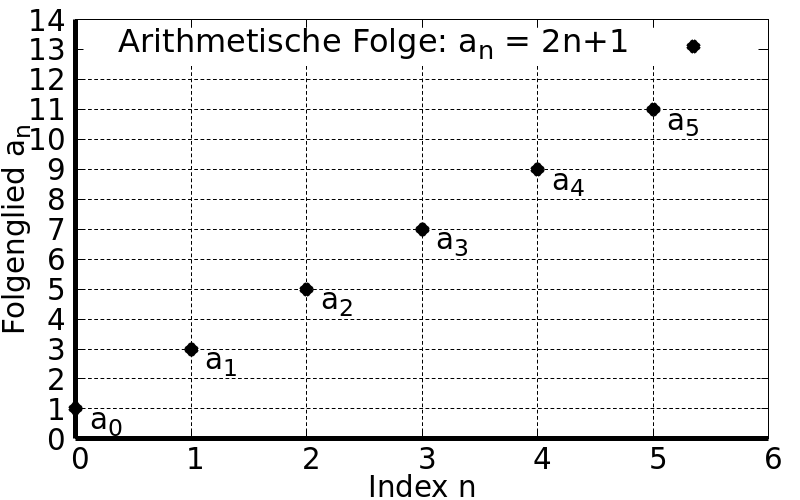
\includegraphics[width=0.8\textwidth]{./gnuplot/example-arithmetic-series.png}
	\caption{Graphische Darstellung der arithmetischen Folge aus \ref{ex:ArithSeq}}
	\label{fig:ExArithSeq}
\end{figure}

\begin{figure}
	\centering
	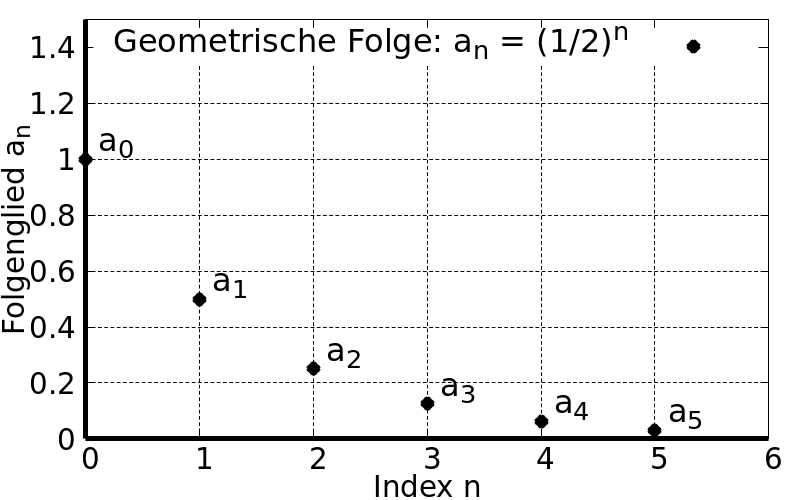
\includegraphics[width=0.8\textwidth]{./gnuplot/example-geometric-series.png}
	\caption{Graphische Darstellung der geometrischen Folge aus \ref{ex:GeoSeq}}
	\label{fig:ExGeoSeq}
\end{figure}

Wie in Abbildung \ref{fig:ExArithSeq} und \ref{fig:ExGeoSeq} dargestellt, lässt sich eine Zahlenfolge auch in einem Diagramm darzustellen. Hierbei ist zu beachten, dass nur Punkte, aber keine durchgehenden Linien eingezeichnet werden dürfen - denn der Definitionsbereich besteht nur aus den natürlichen Zahlen. Ebenfalls diesen beiden Abbildungen lässt sich entnehmen, dass Zahlenfolgen unterschiedlich verlaufen können. Die arithmetische Reihe steigt ohne Grenzen an, die geometrische Reihe $(a_n) = (\frac{1}{2})^n$ fällt und nähert sich immer weiter der $0$ an. Dies gibt Anlass, zwei wichtige Eigenschaften von Zahlenfolgen zu definieren.

\begin{definition}{Monotonie einer Zahlenfolge}{MonoSeq}
	Eine Zahlenfolge $(a_n)$ heißt \textbf{streng monoton wachsend}, wenn jedes Glied größer ist als das vorige, also $\forall n \in\N: a_{n+1} > a_n$ gilt. Analog heißt die Zahlenfolge \textbf{streng monoton fallend}, wenn jedes Glied kleiner ist als das vorige, also $\forall n \in\N: a_{n+1} < a_n$ gilt. Gilt nur $a_{n+1} \ge a_n$ beziehungsweise $a_{n+1} \le a_n$, so spricht man nur von einer \textbf{monoton steigenden} beziehungsweise \textbf{monoton fallenden} Folge (ohne dem Wörtchen "streng").
\end{definition}

\begin{definition}{Beschränktheit einer Zahlenfolge}{BoundSeq}
	Eine Zahlenfolge $(a_n)$ heißt \textbf{nach unten beschränkt}, wenn alle ihre Glieder überhalb einer unteren Grenze liegen, das heißt, wenn es ein $L\in\R$ gibt, sodass $\forall n \in\N: L \ge a_n$ gilt. $L$ heißt dann untere Schranke (lower bound) der Zahlenfolge, geschrieben als $L = \inf a_n$ (Infimum).

	Eine Zahlenfolge $(a_n)$ heißt \textbf{nach oben beschränkt}, wenn alle ihre Glieder unterhalb einer oberen Grenze liegen, das heißt, wenn es ein $U\in\R$ gibt, sodass $\forall n \in\N: L \le a_n$ gilt. $L$ heißt dann obere Schranke (lower bound) der Zahlenfolge, geschrieben als $U = \sup a_n$ (Supremum).
\end{definition}

Anmerkung: Manchmal betrachtet man auch nur die Beschränktheit einer Zahlenfolge ohne die ersten $N$ Glieder und schreibt dann $\inf\limits_{n \ge N} a_n$ beziehungsweise $\sup\limits_{n \ge N} a_n$.

\begin{example}{Eigenschaften der arithmetischen und geometrischen Zahlenfolge}{ArithGeoProp}
	Die arithmetische Zahlenfolge $a_{n+1} = a_n + C, a_0 = k, C > 0$ ist streng monoton steigend, denn $a_{n+1} > a_n$ ist äquivalent zu $a_n + C > a_n$ und weiter $C > 0$, was nach Voraussetzung eine wahre Aussage ist. Weiterhin ist sie nicht nach oben beschränkt (\textbf{unbeschränkt}), da für jede noch so große Zahl $U > 0$ sich durch Umstellung der expliziten Darstellung ein Folgenglied $n'$ finden lässt, sodass $a_{n'} > U$ gilt. Allerdings ist sie nach unten beschränkt, dass alle Glieder größer oder gleich dem Startwert $k$ sind.

	Analog findet man für arithmetische Zahlenfolgen mit $C<0$, dass sie monoton fallend, nach oben beschränkt und nach unten unbeschränkt ist. Für $C=0$ erhält man die sogenannte konstante Folge, welche sowohl mononton steigend als auch fallend ist (aber nicht streng), und sowohl nach oben als auch nach unten beschränkt ist.

	Für die geometrische Zahlenfolge $a_{n+1} = q \cdot a_n, a_0 = p, 0 < q < 1, p > 0$ stellt wir zuerst fest, dass alle ihre Glieder positiv sind. Sie ist streng monoton fallend, denn $a_{n+1} < a_n$ ist äquivalent zu $q \cdot a_n < a_n$ und weiter (da $a_n$ positiv) $q < 1$, was nach Voraussetzung eine wahre Aussage ist. Sie ist nach oben beschränkt, da sie monoton fallend ist. Weiterhin ist sie auch nach unten beschränkt, da alle Folgeglieder positiv sind (und damit $L=0$ eine untere Schranke darstellt).
\end{example}

\section{Konvergenz und Grenzwertbegriff}

Eine weitere Eigenschaft von fundamentaler Bedeutung ist das sogenannte Konvergenzverhalten einer Zahlenfolge. An dem Beispiel der geometrischen Folge $(\frac{1}{2})^n$ in Abbildung \ref{fig:ExGeoSeq} haben wir bereits gesehen, dass sich diese scheinbar immer weiter der $0$ anzunähern scheint, ohne diese jemals (im Endlichen) zu erreichen. Diese Idee, dass eine Folge sich einem Grenzwert immer weiter nähert, wird durch die folgende Definition präzisiert.

\begin{definition}{Konvergenz und Grenzwert}{Convergence}
	Eine Folge $(a_n)$ heißt \textbf{konvergent} mit dem \textbf{Grenzwert} $\alpha$, wenn der Abstand der Folgenglieder zum Grenzwert beliebig klein wird und klein bleibt. Andernfalls heißt sie \textbf{divergent}.

	$\forall \epsilon > 0 \exists n_0\in\N: \forall n > n_0 : |a_n - \alpha| < \epsilon$

	Man schreibt dann: $\lim\limits_{n\to\infty} a_n = \alpha$.
\end{definition}

Anders formuliert kann man auch sagen, die Folge $(a_n)$ heißt konvergent mit dem Grenzwert $\alpha$, wenn man zu jedem noch so kleinen Abstand zum Grenzwert (bezeichnet mit $\epsilon$) immer eine Position in der Zahlenfolge finden kann, sodass alle Folgenglieder rechts von dieser Position innerhalb dieses Abstands liegen. Visuell wird diese Definition durch Abbildung \ref{fig:VisLimit} illustriert.

\begin{figure}
	\centering
	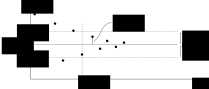
\includegraphics[width=0.8\textwidth]{./svg/definition-convergence.png}
	\caption{Graphische Veranschaulichung des Grenzwertbegriffs}
	\label{fig:VisLimit}
\end{figure}

In Beispiel \ref{ex:ConvGeoSeq} und \ref{ex:ConvConstSeq} wird gezeigt, wie man anhand dieser Definition nachweisen kann, ob eine Folge konvergent ist und welchen Grenzwert sie hat. Ebenfalls wie in Beispiel \ref{ex:ConvAltSeq} kann man zeigen, dass eine Folge divergent ist. Für die praktische Bestimmung von Grenzwerten ist diese Definition sehr umständlich, wir werden daher in Kürze Rechenregeln kennen lernen, um die Berechnung von Grenzwerten zu vereinfachen.

\begin{example}{Konvergenz der geometrischen Folge}{ConvGeoSeq}
	Wir betrachten noch einmal die geometrische Folge $a_n = (\frac{1}{2})^n$. Wir vermuten, dass $\alpha=0$ der Grenzwert ist. Um dies zu beweisen, benutzen wir die obige Definition. Sei $\epsilon>0$. Wir müssen
	nun ein $n_0$ finden, sodass $|a_n-\alpha|=(\frac{1}{2})^n < \epsilon$ gilt, wenn $n > n_0$. Durch Umstellen der Ungleichung erhalten wir $n > \log_{1/2}(\epsilon)$ (man beachte, dass sich das Ungleichheitszeichen umkehrt, da $\log_{1/2}$ eine monoton fallende Abbildung ist). Die Ungleichung ist also erfüllt, solange wir Folgenglieder $a_n$ betrachten, wo $n$ größer als $\log_{1/2}(\epsilon)$ ist. Abschließend setzen wir $n_0 = \floor{\log_{1/2}(\epsilon)}$, wobei die Klammer mit dem unteren Hacken für die Operation "Abrunden" stehen. Damit können wir schreiben:

	$$
	\forall \epsilon > 0 \exists n_0 = \floor{\log_{1/2}(\epsilon)} : \forall n > n_0 : |a_n - 0| < \epsilon
	$$

	Also ist die geometrische Folge $a_n = (\frac{1}{2})^n$ konvergent und hat den Grenzwert $\alpha=\lim\limits_{n\to\infty}(\frac{1}{2})^n=0$.
\end{example}


\begin{example}{Konvergenz der konstanten Folge}{ConvConstSeq}
	Die konstante Folge $a_n = 1$ ist ebenfalls konvergent und hat den Grenzwert $\alpha = 1$, denn für den Abstand gilt $|a_n-\alpha|=|1-1|=0<\epsilon$. Wir erkennen an diesem Beispiel, dass es nicht von Relevant ist, ob die Folgenglieder den Grenzwert erreichen oder nicht -- entscheidend ist lediglich der Abstand zum Grenzwert, und dieser kann auch $0$ betragen kann.
\end{example}


\begin{example}{Divergenz der alternierenden Folge}{ConvAltSeq}
	Die Folge $a_n = (-1)^n$ mit den Gliedern $1,-1,1,-1,...$ heißt alternierende Folge. Diese ist zwar nach oben und unten beschränkt (durch $L=-1$ und $U=1$), besitzt allerdings keinen Grenzwert. Wählt man etwa $\alpha=1$, erhält man für den Abstand $(d_n) = |a_n-\alpha|=(-1)^n-1| = (0, 2, 0, 2, 0, 2)$. Ist $\epsilon$ nun genügend klein, etwa $0.5$, so findet man immer wieder ein Folgenglied, dessen Abstand zum Grenzwert größer ist als $\epsilon$. Egal, welchen Grenzwertkandidaten man wählt, es ist nicht möglich, den Abstand zum Grenzwertkandidaten beliebig klein zu halten.
\end{example}

Ist eine Folge nicht konvergent, so heißt Sie wie erwähnt divergent und besitzt folglich auch keinen Grenzwert. Nun gibt es eine besondere Art der Divergenz, bei der man gelegentlich auch davon spricht, der Grenzwert sei $\pm\infty$. Diese Aussage ist immer im Sinne der folgenden Definition zu verstehen:

\begin{definition}{Bestimmte Divergenz}{Divergence}
	Eine Folge heißt \textbf{bestimmt divergent} gegen $+\infty$ ($-\infty$), falls die Folgenglieder beliebig groß (klein) werden und auch groß (klein) bleiben.

	$$
	\forall R > 0 \exists n_0\in\N: \forall n > n_0 : a_n > R
	$$

	$$
	\forall R < 0 \exists n_0\in\N: \forall n > n_0 : a_n < R
	$$

	Man schreibt dann auch $\lim\limits_{n\to\infty}a_n = +\infty$ beziehungsweise $\lim\limits_{n\to\infty}a_n = -\infty$.
\end{definition}


\begin{example}{Divergenz der arithmetischen Folge}{DivArithSeq}
	Die arithmetische Folge $a_n=2n+1$ ist bestimmt divergent gegen $\infty$. Aus $2n+1 > R$ erhalten wir $n > \frac{R-1}{2}$ Wählen wir nun $n_0 = \floor{\frac{R-1}{2}}$, so können wir schreiben:

	$$
	\forall R > 0 \exists n_0 = \floor{\frac{R-1}{2}}: \forall n > n_0 : a_n > R
	$$

	Es ist also $\lim\limits_{n\to\infty} 2n+1 = \infty$.
\end{example}


\section{Reihe}

Bei einer Reihe handelt es sich um eine ganz bestimmte Form einer Zahlenfolge, die eine eigene Bezeichnung erhalten hat, da sie in der Praxis häufig vorkommt. Etwa wird der von Achilles aufgeholte Vorsprung der Schildkröte in jedem Schritt durch eine geometrische Zahlenfolge beschrieben. Der gesamte zurückgelegte Weg ergibt sich durch Addition der einzelnen Teilwege und stellt eine geometrische Reihe dar.

\begin{definition}{Begriff der Reihe}{Series}
	Eine \textbf{Reihe} $(s_n)$ entsteht durch Summation der Glieder einer Zahlenfolge. Die Summe $s_n=\sum\limits_{i=0}^n a_i$ der ersten $(n+1)$-Glieder heißt \textbf{Partialsumme}. Der Grenzwert der Partialsummen, falls existent, $s_\infty = \lim\limits_{n\to\infty}s_n$ heißt \textbf{unendliche Reihe}.
\end{definition}

Anhand der arithmetischen und geometrischen Folge und der daraus induzierten Reihe wird der Reihenbegriff in den Beispielen \ref{ex:PartSumArithSer} und \ref{ex:PartSumGeoSer} verdeutlicht.

\begin{example}{Partialsummen der arithmetischen Reihe}{PartSumArithSer}
	Die arithmetische Reihe $a_n = k\cdot n+m$ mit $k,m\in\R$ ist für $k \ne 0$ unbeschränkt, die unendliche Reihe wird daher nicht existieren. Die Partialsummen lauten $s_n = \sum\limits_{i=0}^n (ki+m)$. Durch Anwendung des Assoziativ- und Distributivgesetzes können wir dies umformen zu $\left(k\cdot\sum\limits_{i=0}^n i\right) + \left(\sum\limits_{i=0}^n m\right)$. Die rechte Summenbildung stellt lediglich die Addition der $(n+1)$ konstanten Zahlen $m$ dar und beträgt mithin $m\cdot(n+1)$.

	Für die linke Summe $\sum\limits_{i=0}^n i$ müssen wir die ersten $n$ natürlichen Zahlen aufaddieren. Hierzu bedienen wir uns eines Verfahrens, welches unter anderem durch \mention{Carl Friedrich Gauß} bekannt geworden ist. Um die Zahlen von $1$ bis $100$ zu addieren, teilte er die Summe auf in Paare: $1+100$, $2+99$, $3+98$, $4+97$ und so fort. Jedes Paar hat den Wert $101$, ingesamt gibt es $50$ Paare. Damit beträgt die Summe $50\cdot 101 = 5050$. Allgemein gilt, das wenn die Zahlen von $1$ bis $n$ zu addieren sind, es dann $n/2$-Paare mit jeweils dem Wert $n+1$ gibt und deren Summe $\frac{n(n+1)}{2}$ beträgt.

	Man beachte dabei den Fall, wenn $n$ ungerade ist, also ein ungerade Anzahl an Zahlen zu addieren ist. Dann gibt es nur $(n-1)/2$-Paare mit der Summe $(n+1)$ und die mittlere Zahl $(n+1)/2$ bleibt übrig. Letzlich beträgt die Summe somit ebenfalls $\frac{n-1}{2}(n+1)+\frac{n+1}{2} = \frac{n(n+1)}{2}$.

	Insgesamt gewinnen wir für die Partialsummen somit den Ausdruck:

	\begin{equation}
	  s_n = k \frac{n(n+1)}{2} + m\cdot(n+1) = \frac{k}{2}n^2 + \left(m+\frac{k}{2}\right)n + m
	\end{equation}

	Beispielsweise können wir anhand dieser Formel berechnen, dass die Summe der ungeraden Zahlen kleiner $100$ lautet

	$$
	  1+3+5+...+97+99 = \sum\limits_{n=0}^{49} 2n+1 = 2\frac{49\cdot 50}{2} + 50 = 2500
	$$
\end{example}

\begin{example}{Partialsummen der geometrischen Reihe}{PartSumGeoSer}
	Die geometrische Folge lautet $a_n = p \cdot q^n$ mit $p,q\in\R$. Um die Partialsummen $s_n = \sum\limits_{i=0}^n p\cdot q^i$ zu bestimmen, bedienen wir uns eines kleinen Umformungstricks. Die Partialsumme wird mit der konstanten $q$ multipliziert und von der ursprünglichen Partialsumme abgezogen, sodass sich fast alle Summanden aufheben:

	\begin{alignat*}{4}
		        s_n       &= p \cdot ( & q^0 + & q^1 + q^2 + q^3 + ... + q^n           &) \\
		q \cdot s_n       &= p \cdot ( &       & q^1 + q^2 + q^3 + ... + q^n + q^{n+1} &)
	\end{alignat*}
	\begin{alignat*}{1}
		s_n - q \cdot s_n &= p \cdot (1 - q^{n+1}) \\
          s_n \cdot (1-q) &= p \cdot (1 - q^{n+1})
	\end{alignat*}

	Die letzte Gleichung können wir nun direkt nach der gesuchten Partialsumme $s_n$ umstellen und erhalten:

	\begin{equation}
	  s_n = p \frac{1 - q^{n+1}}{1 - q}
	\end{equation}

	Mithilfe dieser Formel können wir nun beispielsweise die Summe aller Inversen von Zweierpotenzen berechnen:

	$$
	 1 + \frac{1}{2} + \frac{1}{4} + \frac{1}{8} + ... + \frac{1}{256} = \sum\limits_{n=0}^8 (\frac{1}{2})^n = \frac{1 - (1/2)^9}{1/2} = \frac{1022}{512} = \frac{511}{256}
	$$
\end{example}

\begin{example}{Grenzwert der geometrischen Reihe}{LimGeoSer}
    Die Partialsummen der geometrischen Reihe lauten $s_n = p \frac{1 - q^{n+1}}{1 - q}$. Für welche Werte von $p$ und $q$ konvergieren diese bei $n\to\infty$. Die meisten Terme in der Partialsumme sind unabhängig von $n$, der einzige von $n$ abhängige Term lautet $q^{n+1}$ und ist selbst wieder eine geometrische Folge. Diese konvergiert für $|q| < 1$ gegen $0$. Für $q=1$ ist die geometrische Reihe $1+1+1+\dots$ offensichtlich divergent. Somit ist die geometrische Reihe konvergent für $|q|<1$ und hat den Grenzwert:
    $$
        s_\infty = \lim\limits_{n\to\infty} \sum\limits_{i=0}^n p\cdot q^i = \frac{p}{1-q}
    $$
    Es ergibt sich also beispielsweise $1 + \frac{1}{2} + \frac{1}{4} + \frac{1}{8} + ... = \frac{1}{1/2} = 2$.
\end{example}

\section{Konvergenz von Folgen}

Wir haben bereits die formale Definition von Konvergenz kennengelernt. Auch haben wir gesehen, dass man zwar anhand dieser Definition Grenzwert bestimmen kann, dies meist aber nur recht umständlich möglich ist. Für die praktische Berechnung von Grenzwerten wollen wir uns daher noch einige Rechenregeln anschauen, welche die Rechenarbeit erleichtern.

Komplexe Terme sind durch Rechenoperationen aus einfacheren Termen aufgebaut. Zuerst benötigen wir die Grenzwerte einiger spezieller Terme. Diese seien im Folgenden ohne Beweis angegeben:

\begin{statement}{Grenzwerte einiger spezieller konvergenter Folgen}{LimSpecSeq}
	Die folgenden Folgen sind konvergent und haben den angegeben Grenzwert.
	\begin{alignat}{3}
		& \lim\limits_{n\to\infty} & \frac{1}{n^q}  & = 0, q > 0 \label{eq:LimitInv1nq} \\
		& \lim\limits_{n\to\infty} & q^n & = 0, |q| < 1 \\
		& \lim\limits_{n\to\infty} & \nroot{n}{n} & = 1 \\
		& \lim\limits_{n\to\infty} & \nroot{n}{q} & = 1, q > 0 \\
		& \lim\limits_{n\to\infty} & \frac{a^n}{n!} & = 0, a \in \R \label{eq:LimitPowerFactorial} \\
		& \lim\limits_{n\to\infty} & \left(1+\frac{1}{n}\right)^n & = e \label{eq:LimitExp}
	\end{alignat}
\end{statement}

Ein wichtiger Satz, der manchmal bei schwierigen Grenzwerten hilft, ist das sogenannte \emph{Sandwich-Kriterium}. Schafft man es zu zeigen, dass eine Folge zwischen zwei anderen Folgen liegt, so muss auch der Grenzwert der Folgen zwischen den Grenzwerten der anderen beiden Folgen liegen. Haben diese beiden Folgen den gleichen Grenzwert, kennt man damit den Grenzwert der zu untersuchenden Folge.

\begin{statement}{Sandwich-Kriterium}{SandwichTheo}
	Gegeben sei eine Folge $(a_n)$. Gibt es zwei konvergente Folgen $(l_n)$ und $(u_n)$, die beide gegen den gleichen Grenzwert $\alpha$ konvergieren, und gilt ab einem bestimmten Folgenglied $n_0$ die Ungleichung $l_n \le a_n \le u_n, n \ge n_0$, dann konvergiert auch die Folge $a_n$ gegen $\alpha$.
\end{statement}

\begin{example}{Anwendung des Sandwich-Kriteriums}{SandwichTheo}
	Gesucht ist der Grenzwert der Folge $a_n = \frac{1}{n^2}\sin(n)$. Von den elementaren Eigenschaften der Sinusfunktion wissen wir, dass gilt $-1\le\sin(n)\le 1$. Wählen wir nun $l_n = -\frac{1}{n^2}$ und $u_n = \frac{1}{n^2}$, so gilt $l_n \le a_n \le u_n$. Die Folge $a_n$ wird also durch die zwei Folgen $(l_n)$ und $(u_n)$ eingeschachtelt. Für diese beiden Folgen gilt nach \ref{eq:LimitInv1nq} $\lim\limits_{n\to\infty} \pm\frac{1}{n^2} = 0$. Nach dem Sandwich-Kriterum \ref{stmt:SandwichTheo} folgt somit $\lim\limits_{n\to\infty} \frac{1}{n^2}\sin(n) = 0$.
\end{example}

Folgende Regeln gelten, wenn eine neue Folge durch Addition oder Multiplikation der Glieder zweier anderer Folgen gebildet wird:

\begin{statement}{Grenzwertregeln für zusammengesetzte Folgen}{CombSeqLimit}
	Seien $(a_n), (b_n), (c_n)$ konvergente Zahlenfolgen mit jeweils dem Grenzwert $a, b, c$ und $c_n, c \ne 0$. Sei zudem $c \in \R$ eine Konstante und $f: \R\to\R$ eine stetige Funktion. Dann gelten die folgenden Rechenregeln für Grenzwerte:

	\begin{alignat}{2}
		& \lim\limits_{n\to\infty}(a_n \pm b_n) & = a + b \label{eq:LimSum} \\
		& \lim\limits_{n\to\infty}(a_n \cdot b_n) & = a \cdot b \label{eq:LimProd} \\
		& \lim\limits_{n\to\infty}(a_n / c_n) & = a / c \label{eq:LimQuot} \\
		& \lim\limits_{n\to\infty}(c \cdot a_n) & = c \cdot a \label{eq:LimCoeff} \\
		& \lim\limits_{n\to\infty}(f(a_n)) & = f(a)	\label{eq:LimFun}
	\end{alignat}
\end{statement}

Gleichung \ref{eq:LimSum} und \ref{eq:LimProd} sagen aus, dass bei einem Grenzwert von Summen und Produkten die Grenzwerte der Summanden und Faktoren einzeln betrachtet werden können. Gleichung \ref{eq:LimCoeff} ist eine einfache Konsequenz aus \ref{eq:LimProd}. Die letzte Gleichung \ref{eq:LimFun} sagt aus, dass bei Anwendung einer (stetigen) Funktionen auf die Glieder einer Zahlenfolge die Grenzwertbildung in das Funktionsargument gezogen werden kann.	Übrig bleibt Gleichung \ref{eq:LimQuot}, welche analog zu den ersten beiden Gleichungen aussagt, dass auch bei einer Quotientenbildung die Grenzwerte von Dividend und Divisor einzeln betrachtet werden können. Allerdings muss hier die wichtige Einschränkung beachtet werden, dass die Glieder und der Grenzwert des Divisors ungleich $0$ sind, da die Division durch $0$ nicht erklärt ist. Nun gibt es aber speziell Folgen von Quotienten, wo die Glieder des Divisors zwar ungleich $0$ sind, der Grenzwert des Divisors aber nicht.

In \ref{ex:CombSeqLimit} sind einige für die ersten vier Regeln zusammengefasst.

\begin{example}{Anwendung der Grenzwertregeln für zusammengesetzte Folgen}{CombSeqLimit}
    \begin{itemize}
        \item $\lim\limits_{n\to\infty} \frac{n^2+1}{n^3} = \lim\limits_{n\to\infty} \left(\frac{1}{n} + \frac{1}{n^3}\right) = 0 + 0 = 0$ \\
        \item $\lim\limits_{n\to\infty} \frac{n-2}{n^2-3n+2} = \lim\limits_{n\to\infty} \frac{n(1-2/n)}{n^2(1-3/n+2/n^2)} = \lim\limits_{n\to\infty} \frac{1}{n} \cdot \frac{1-2/n}{1-3/n+2/n^2} = 0 \cdot \frac{1-0}{1-0+0} = 0$ \\
        \item $\lim\limits_{n\to\infty} \frac{n^2+1}{n-1} = \lim\limits_{n\to\infty} \frac{n^2(1+2/n^2)}{n(1-1/n)} = \lim\limits_{n\to\infty} n \cdot \frac{1+2/n^2}{1-1/n} = \infty $
        \item $\lim\limits_{n\to\infty} \frac{4n^3+2n}{7n^3-4n^2} = \lim\limits_{n\to\infty} \frac{n^3(4+2/n^2)}{n^3(7-4/n)} = 1 \cdot \frac{4+0}{7-0} = \frac{4}{7}$
    \end{itemize}
\end{example}

Die Anwendung der Rechenregel \ref{eq:LimFun} wird in Beispiel \ref{ex:LimFun} verdeutlicht.

Um auch Grenzwerte von Quotienten berechnen zu können, wo der Divisor gegen $0$ konvergiert, hilft die folgende Aussage. Dazu benötigen wir noch zwei Definitionen.

Bisher haben wir nur Grenzwerte betrachtet, wo $n$ gegen $\infty$ lief. Es ist nun aber so, dass man Grenzwerte nicht nur für Folgen, sondern auch für Funktionen betrachten kann, wenn das Funktionsargument sich einem bestimmten Wert (nicht zwingend $\infty$) nähert.

\begin{definition}{Grenzwert einer Funktion}{LimFun}
    Sei $f: \R^n \to \R$ eine Funktion, welche $n$-dimensionale Punkte auf reelle Zahlen abbildet, und sei $x_0\in\R^n$ eine Stelle des Definitionsbereichs. Die Zahl $\alpha\in\R$ heißt Grenzwert von $f$ gegen $x_0$, wenn es für jede noch so kleine Epsilon-Kugel um $\alpha$ eine Delta-Kugel um $x_0$ gibt, sodass die Funktionswerte der Delta-Kugel in der Epsilon-Kugel liegen.
    $$
        \forall \epsilon > 0 \exists \delta > 0 : f(S_\delta(x_0)) \subset S_\epsilon(\alpha)
    $$
    Man schreibt dann $\lim\limits_{x\to x_0} = \alpha$.
\end{definition}

Graphisch ist diese Definition dargestellt in Abbildung \ref{fig:LimFun} und bedeutet anschaulich, dass kleine Änderungen des Arguments immer nur kleine Änderungen des Funktionswerts zur Folge haben. Äquivalent zu dieser Definition ist, dass für jede gegen $x_0$ konvergent Folgen $a_n$ auch die Folge $f(a_n)$ der Funktionswerte gegen $\alpha$ konvergieren muss. Wenn der Grenzwert existiert, dann kann man ihn dadurch bestimmen, indem man die Grenzwertbildung für die einzelnen Variablen ($x_1, x_2, \dots$) der Reihe nach ausführt.

\begin{figure}
    \centering
    
\includegraphics[width=0.55\textwidth]{./svg/definition-convergence-point}
    \caption{Grenzwert einer Funktion an einer Stelle $x_0$}
    \label{fig:LimFun}
\end{figure}

Die Grenzwertregeln, die wir bisher kennengelernt haben, sind analog auch auf Grenzwerte von Funktionen übertragbar.

\begin{example}{Grenzwertregeln für Grenzwert einer Funktion}{LimFunSumQuot}
    Auf $\lim\limits_{x\to 0} \frac{x^2+x+2}{x^3+1}$ lassen sich analog die Grenzwertregeln \ref{eq:LimSum} und \ref{eq:LimQuot} anwenden und man erhält: $\frac{0^2+0+2}{0^3+1} = 2$.
\end{example}

\begin{example}{Nichtexistenz des Grenzwerts einer einstelligen Funktion}{CheckLimUnivarFun}
    Die einstellige Funktion $f: x \mapsto \sin(1/x)$ hat keinen Grenzwert für $x \to 0$. Je nachdem, wir wir uns $0$ nähern, erhält man verschiedene Ergebnisse. Beispielsweise können wir die Folgen $a_n = \frac{2}{\pi+4\pi n}$ und $b_n = \frac{1}{\pi n}$. Diese konvergieren beiden gegen $0$. Allerdings gilt für die Folgen der Funktionswerte:
    \begin{alignat}{1}
       \lim\limits_{n\to\infty} f(a_n) &= \lim\limits_{n\to\infty} \sin\left(1 / \frac{2}{\pi+4\pi n}\right) = \lim\limits_{n\to\infty} \sin(\frac{\pi}{2} + 2\pi n) = 1 \\
       \lim\limits_{n\to\infty} f(b_n) &= \lim\limits_{n\to\infty} \sin\left(1 / \frac{1}{\pi n}\right) = \lim\limits_{n\to\infty} \sin(\pi n) = 0 \\
    \end{alignat}
    Wir erhalten verschiedene Werte, somit existiert der Grenzwert nicht.
\end{example}

\begin{example}{Nichtexistenz des Grenzwerts einer mehrstelligen Funktion}{CheckLimMultivarFun}
    Die mehrstellige Funktion $f: (x,y) \mapsto \frac{x^2-y^2}{x^2+y^2}$ hat keinen Grenzwert für $(x_0,y_0) \to (0,0)$. Je nachdem, auf welchem Weg wir uns $(0,0)$ annähern, erhalten wir verschiedene Grenzwerte. Wenn wir uns dem Koordinatenursprung etwa nähern, indem wir erst zur x-Achse $y=0$ gehen, erhalten wir:
    $$
    \lim\limits_{x\to 0} \lim\limits_{y\to 0} \frac{x^2-y^2}{x^2+y^2} = \lim\limits_{x\to 0} \frac{x^2}{x^2} = 1
    $$
    Andererseits gilt, wenn wir erst zur y-Achse $x=0$ gehen:
    $$
    \lim\limits_{y\to 0} \lim\limits_{x\to 0} \frac{x^2-y^2}{x^2+y^2} = \lim\limits_{y\to 0} \frac{-y^2}{y^2} = -1
    $$
    Wir erhalten verschiedene Werte, somit existiert der Grenzwert nicht.
\end{example}

\begin{statement}{Grenzwert gebrochenrationaler Funktionen}{LimRatFun}
    Aus den bisherigen Beispielen können wir die folgende allgemeine Regel ableiten, die für den Grenzwert eines Quotienten von Polynomen gilt:
    Sei $f(x) = \frac{p_n(x)}{q_m(x)}$ eine gebrochenrationale Funktion, also der Quotient zweier Polynome $p_n, q_m$ vom Grad $n$ und $m$. Der Grenzwert existiert, wenn der Grad des Zählerpolynoms nicht kleiner ist als der Grad des Nennerpolynoms. Es gilt:

    \begin{equation}
    \lim\limits_{x\to\infty}\frac{p_n(x)}{q_m(x)} = \lim\limits_{x\to\infty}\frac{a_0 + a_1 x + a_2 x^2 + ... + a_n x^n}{b_0 + b_1 x + b_2 x^2 + ... + b_n x^n} = \begin{cases}
    0 &\text{falls $n < m$} \\
    \frac{a_n}{b_m} &\text{falls $ n = m$} \\
    \pm \infty  &\text{falls $ n > m$}
    \end{cases}
    \end{equation}

    Das Vorzeichen für den letzten Fall ergibt sich aus dem Vorzeichen der höchsten Koeffizienten $a_n$ und $b_n$. Sind beide positiv oder negativ, divergiert $f$ bestimmt gegen $+\infty$. Haben sie verschiedenes Vorzeichen, divergiert $f$ bestimmt gegen $-\infty$.
\end{statement}

Für die nächste Grenzwertregel benötigen wir weiterhin noch das Konzept der sogenannten \emph{unbestimmten Ausdrücke}.

\begin{definition}{Unbestimmte Ausdrücke}{IndetForms}
	Wir sprechen von einem \textbf{unbestimmten Ausdruck}, wenn eine Zahlenfolge aus zwei mit einer Rechenoperation verknüpften konvergenten oder bestimmt divergenten Einzelfolgen besteht, die obigen Grenzwertregeln aber nicht anwendbar sind.

	Die \textbf{Form des unbestimmten Ausdrucks} erhält man, indem man die Grenzwerte der Einzelfolgen mit der Rechenoperation verknüpft aufschreibt.
\end{definition}

Einige Beispiele für solche unbestimmten Ausdrücke finden sich in \ref{ex:IndetForms}. An diesesr Stelle sei noch eine Anmerkung angebracht: Manchmal spricht man davon, dass $1/0$ "unendlich" sei. Dies ist so aber nicht korrekt. Zum einen ist ein Ausdruck der Form $1/0$ immer nur als unbestimmter Ausdruck zu verstehen. Zum zweiten verbirgt sich hinter einem unbestimmten Ausdruck immer ein Grenzwert. Nur, wenn jeder Grenzwert der Form $1/0$ konvergent (oder bestimmt divergent) mit dem gleichen Grenzwert wäre, ließe sich diese Aussage rechtfertigen. Nun ist aber $\lim\limits_{n\to\infty} \frac{1}{1/n} = \infty$ und $\lim\limits_{n\to\infty} \frac{1}{-1/n} = -\infty$, beide sind aber unbestimmte Ausdrücke der Form $1/0$. Gleiches gilt für den unbestimmten Ausdruck $0^0$ -- je nach Wahl der konkreten Zahlenfolgen erhält man hier verschiedene Grenzwerte.

\begin{example}{Unbestimmte Ausdrücke}{IndetForms}
	\begin{itemize}
		\item $\lim\limits_{x\to\infty} \frac{\sin(n)}{e^x}$ ist ein unbestimmter Ausdruck der Form $\frac{\infty}{\infty}$
		\item $\lim\limits_{x\to\infty} e^{-x} \cdot x^2$ ist ein unbestimmter Ausdruck der Form $0 \cdot \infty$.
		\item $\lim\limits_{x\to 0} x^x$ ist ein unbestimmter Ausdruck der Form $0 ^ 0$.
	\end{itemize}
\end{example}

Mit diesem Wissen lässt sich nun die nächste Rechenregel formulieren.

\begin{statement}{Regel von L'Hôpital}{HopitalRule}
	Seien $f,g: \R\to\R$ zwei differenzierbare Funktionen und ist $\lim\limits_{n\to x_0} \frac{f(x)}{g(x)}$ ein unbestimmter Ausdruck der Form $\frac{0}{0}$ oder $\frac{\infty}{\infty}$, dann gilt:

    \begin{equation}
        \lim\limits_{x \to x_0} \frac{f(x)}{g(x)} = \lim\limits_{x \to x_0} \frac{f'(x)}{g'(x)}
    \end{equation}

    Voraussetzung hierbei ist, dass der rechte Grenzwert existiert. Aus der Nichtexistenz des rechten Grenzwerts \textbf{darf nicht} auf die Nichtexistenz des ursprünglichen Grenzwerts geschlossen werden.
\end{statement}

\begin{example}{Anwendung der Regel von L'Hôpital}{HopitalRule}
    \begin{itemize}
        \item $\lim\limits_{x\to\infty} \frac{\ln(x)}{x^2} = \lim\limits_{x\to\infty} \frac{1/x}{2x} = \lim\limits_{x\to\infty} \frac{1}{2x^2} = 0$
        \item $\lim\limits_{x\to\infty} x \cdot \ln(x) = \lim\limits_{x\to\infty} \frac{\ln(x)}{1/x} = \lim\limits_{x\to\infty} \frac{1/x}{-1/x^2} = 0$
        \item $\lim\limits_{x\to\infty} \frac{\sin(x)}{x} = \lim\limits_{x\to\infty} \frac{\cos(x)}{1} = \cos(0) = 1$
    \end{itemize}
\end{example}

\begin{example}{Vertauschung von Grenzwert und Funktionsanwendung}{LimFun}
    Gesucht ist der Grenzwert $\alpha = \lim\limits_{x\to 0^+} x^x$. Dabei bedeutet $x\to 0^+$, dass nur nicht-negative Funktionsargumente betrachtet werden, da $x^x$ sonst nicht erklärt ist, dies nennt man auch \emph{rechtsseitiger Grenzwert}. Wir wenden den Logarithmus auf beide Seiten der Gleichung an, und machen dann von der Rechenregel \ref{eq:LimFun} Gebrauch:
    \begin{alignat*}{1}
        \alpha      & = \lim\limits_{x\to 0^+}  x^x \\
        \ln(\alpha) & = \ln\left(\lim\limits_{x\to 0^+}  x^x \right) \\
                    & = \lim\limits_{x\to 0^+} \ln(x^x) \\
                    & = \lim\limits_{x\to 0^+} x\ln(x)
    \end{alignat*}
    Aus dem vorigen Beispiel \ref{ex:HopitalRule} wissen wir bereits, dass der letzte Grenzwert $0$ beträgt. Damit ergibt sich $\ln(\alpha) = 0$, woraus sofort für den Grenzwert folgt:

    $$
        \lim\limits_{x\to 0^+} x^x = e^0 = 1
    $$
\end{example}

Auf die gleiche Weise wie in Beispiel \ref{ex:LimFun} erhält man auch $\lim\limits_{x\to 0^+} x^{r / \ln(x)} = e^r$ für $r \in \R$. Dies zeigt erneut, dass man dem unbestimmten Ausdruck $0^0$ keinen einzelnen Wert zuordnen kann. Für jedes $r\in\R$ ist der Grenzwert von der Form $0^0$, doch der Grenzwert kann durch $r$ auf jede positive Zahl festgelegt werden.

\section{Konvergenz von Reihen}

Reihen stellen wir erwähnt eine spezielle Form von Zahlenfolge dar. Damit sind auch alle Regeln für die Konvergenz von Zahlenfolgen anwendbar. Zusätzlich gibt es speziell für Reihen noch einige weitere Regeln, die im Folgenden noch kurz angegeben werden sollen.

\begin{statement}{Notwendige Bedingung für die Konvergenz einer Reihe}{ConvSerNecc}
    \textbf{Notwendige Bedingung} für die Konvergenz einer Reihe $s_n = \lim\limits_{n\to\infty} a_n$ ist, dass ihre Glieder eine Nullfolge bilden, also $\lim\limits_{n\to\infty} a_n = 0$ gilt.
\end{statement}

Allerdings ist diese Bedingung nicht ausreichend. Es kann sein, dass die die Glieder einer Zahlenfolge sich gegen $0$ nähern, ihre Summe aber dennoch unbeschränkt wächst. Beispielsweise stellt die Folge $a_n = \frac{1}{n}$ eine Nullfolge dar. Es lässt sich aber zeigen, dass $1 + \frac{1}{2} + \frac{1}{3} + \frac{1}{4} + ...$ unbeschränkt ist und bestimmt gegen $\infty$ divergiert.

Zwei Kriterien, die bei der praktischen Entscheidung, ob eine Reihe konvergent ist, sind das sogenannte Quotienten- und Wurzelkriterium. Diese beruhen darauf, die zu untersuchende Reihe ähnlich zum Sandwich-Kriterium \ref{stmt:SandwichTheo} durch eine bekannt Reihe nach oben abzuschätzen, von der bekannt ist, dass sie konvergiert.

\begin{statement}{Quotientenkriterium}{RatioTest}
    Sei $a_n$ eine konvergente Nullfolge und $s_n = \lim\limits_{n\to\infty} a_n$ die zugehörige Reihe. Existiere weiterhin der Grenzwert $q = \lim\limits_{n\to\infty} |\frac{a_{n+1}}{a_n}|$ des Quotienten aufeinanderfolgender Glieder. Dann gilt:

    \begin{itemize}
        \item $s_n$ ist konvergent für $q < 1$.
        \item $s_n$ ist divergent für $q > 1$.
    \end{itemize}

    Für $q=1$ ist keine Aussage möglich.
\end{statement}


\begin{statement}{Wurzelkriterium}{RootTest}
    Sei $a_n$ eine konvergente Nullfolge und $s_n = \lim\limits_{n\to\infty} a_n$ die zugehörige Reihe. Existiere weiterhin der Grenzwert $q = \lim\limits_{n\to\infty} \nroot{n}{|a_n|}$. Dann gilt:

    \begin{itemize}
        \item $s_n$ ist konvergent für $q < 1$.
        \item $s_n$ ist divergent für $q > 1$.
    \end{itemize}

    Für $q=1$ ist keine Aussage möglich.
\end{statement}

Diese beiden Kriterien werden später noch einmal im Zusammenhang mit Potenzreihen und der sogenannten Taylorentwicklung eine wichtige Rolle spielen.

\begin{example}{Anwendung des Quotientenkriteriums}{RatioTest}
    Untersucht werden soll, ob $s_n = \sum\limits_{i=1}^\infty \frac{n!}{n^n}$ existiert. Das Wurzelkriterium liefert (Betragsstriche sind weggelassen, da alle Glieder positiv):

    \begin{alignat*}{1}
        q &= \lim\limits_{n\to\infty} \frac{(n+1)! \cdot n^n}{(n+1)^{n+1} \cdot n!} \\
          &= \lim\limits_{n\to\infty} \frac{n^n}{(n+1)^n} \\
          &= \lim\limits_{n\to\infty} \left(\frac{n}{n+1}\right)^n \\
          &= \lim\limits_{n\to\infty} \left( \frac{1}{1+1/n} \right)^n \\
          &= \frac{1}{e}
    \end{alignat*}

    Letzteres Gleichheitszeichen folgt aus \ref{eq:LimitExp}. Da $2\le e \le 3$ gilt, können wir für $q$ die Abschätzung vornehmen: $\frac{1}{3} \le q \le \frac{1}{2}$. Damit haben wir gezeigt, dass $q < 1$, somit ist die Reihe $s_n$ konvergent.
\end{example}


% Functions, properties, graphs, multivariate functions
% Special function, polynomns, rational functions
\chapter{Ein- und mehrstellige Funktionen}

Funktionen oder Abbildungen sind die wesentlichen mathematischen Objekte, die in der Analysis und Infinitesimalrechnung untersucht werden. Sie sind deshalb auch von besondere praktischer Bedeutung, da sich mit ihnen Zusammenhänge in den Naturwissenschaften modellieren lassen. Solche Zusammenhänge der realen Welt sind meist komplex, eine untersuchte Größe hängt meist nicht nur von einem, sondern von vielen Faktoren ab. Etwa hängt der elektrische Widerstand von Spannung und Stromstärke ab, der Luftdruck von drei Raum- und einer Zeitkoordinaten. Dementsprechend definiert man auch sogenannte mehrstellige Funktionen, welche mehr als ein Argument aufweisen. In diesem Kapitel werden wir zuerst den Funktionsbegriff näher definieren und anschließend einige ausgewählte wichtige Eigenschaften von Funktionen beleuchten.

\section{Funktionsbegriff}

\begin{definition}{Begriff der Funktion}{Function}
    Eine \textbf{Funktion} $f$ ist eine eindeutige Abbildung beziehungsweise Zuordnung von Elementen einer Grundmenge $\mathbb{S}$ zu Elementen einer Bildmenge $\mathbb{C}$. Die Elemente der Grundmenge heißen \textbf{Argumente}, die Elemente der Bildmenge \textbf{Funktionswerte}. Eindeutigkeit meint hierbei, dass keinem Argument mehr als ein Funktionswert zugeordnet ist.

    Wird jedem Argument ein Funktionswert zugeordnet, spricht man von einer \textbf{totalen Funktion}. Besteht die Zuordnung nur für manche Argumente, spricht man von einer \textbf{partiellen Funktion}. Die Menge $\mathbb{D} \subseteq \mathbb{S}$, für die ein Funktionswert erklärt ist, heißt Definitionsbereich.

    Man schreibt: $f: \mathbb{S} \to \mathbb{C}$.
\end{definition}

Diese Definition macht noch keine Aussage darüber, von welcher Art die Elemente sind. Wählt man reelle Zahlen als Elemente, erhält man die aus der Schulmathematik bekannten reellwertige Funktion. Es können aber auch Abbildungen anderer Elemente betrachtet werden. Beispielsweise werden in der Booleschen Algebra logische Verknüpfungen (\emph{and}, \emph{or}) als Abbildung zwischen Wahrheitswerten (\emph{true}, \emph{false}) betrachtet. Der Differentialoperator ist eine Abbildung auf Funktionen, die einer Funktion ihre Ableitung zuweist.

An dieser Stelle eine wichtige Anmerkung zum Funktionsbegriff. Der mathematische Funktionsbegriff darf nicht mit dem Funktionsbegriff in der Programmierung verwechselt werden. Eine mathematische Funktion ist deterministisch in dem Sinne, das der Rückgabewert vollständig vom Ein- oder Übergabewert abhängt. Dies ist in der Programmierung nicht üblich -- dort kann der Rückgabewert etwa auch von globalen Konstanten, Umgebungsvariablen, Input-Operationen oder bei Methoden in der objektorientierten Programmierung auch vom aktuellen Zustand des Objekt abhängen. Weiterhin sind mathematische Funktionen pur, sie liefern einen Wert zurück und machen sonst nichts. Andererseits können Funktionen in der Programmierung noch sogenannten \emph{Seiteneffekte} aufweisen, etwa das Senden eines \mention{Http}-Requests, das Modifizieren eines Zustands, oder das Schreiben von Log-Ausschriften. Ein Programmier-Paradigma, dass sich stark an mathematischen Funktionen anlehnt, ist die \emph{funktionale Programmierung}.

\begin{example}{Definitionsbereich und Wertebereich}{DomainCodomain}
    Durch die Zuweisung $x\mapsto\frac{1}{x}$ ist eine Abbildung $f: \R \to \R$ zwischen reellen Zahlen definiert. Für die Zahl $0$ ist keine Zuordnung möglich, da hier der Ausdruck $1/0$ nicht erklärt ist. Es handelt sich also um eine partielle Funktion mit dem Definitionsbereich $\mathbb{D} = \lbrace x \in \R | x \ne 0 \rbrace = \R \setminus \lbrace 0 \rbrace$. Außer der $0$ kann jeder Funktionswert angenommen werden, mithin lautet der Wertebereich ebenfalls $\mathbb{C} = \R \setminus \lbrace 0 \rbrace$.
\end{example}

Eine wichtige Funktion ist die Identität, welche jedes Argument sich selbst zuordnet.

\begin{definition}{Identitätsfunktion}{IdFun}
    Sei $M$ eine Menge. Die Funktion $id_M: M \to M$ heißt \textbf{Identitätsfunktion} auf der Menge $M$ und ist gegeben durch $id_M: x \mapsto x$.
\end{definition}

Sie wird auch geschrieben als $\mathbbm{1}_M$ geschrieben, oder, wenn die Menge $M$ aus dem Kontext heraus bekannt ist, auch nur als $id$ beziehungsweise $\mathbbm{1}$.

Unabhängig der Art der Elemente besteht eine Möglichkeit zur Veranschaulichung von Funktionen in der Darstellung als Wertetafel oder Pfeildarstellung wie in Abbildung \ref{fig:FunAsArrows}. Links in der Abbildung ist eine Funktion $f: \N \to \N$ dargestellt, die jeder natürlichen Zahl ihre Quadratzahl zuweist. Rechts ist der boolesche Operator \emph{Exklusives Oder} abgebildet, der eine Funktion zwischen einem Paar von Wahrheitswerten zu einem Wahrheitswert ist.

\begin{figure}[h]
    \label{fig:FunAsArrows}
    \centering
    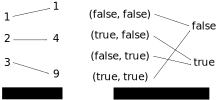
\includegraphics[width=0.8\textwidth]{./svg/function-as-arrows}
    \caption{Darstellung von Funktionen als Pfeildiagramm}
\end{figure}

Für diese Vorlesung beschränken wir uns auf Funktionen zwischen reellen Zahlen. Hier unterscheiden wir zwei Arten, je nachdem, ob der Funktionswert nur von einer reellen Zahl oder von mehreren abhängt.

\begin{definition}{Einstellige Funktion}{UnivarFun}
    Von einer \textbf{einstelligen reellwertigen Funktion} spricht man, wenn eine Abbildung $f: \R \to \R$ von einer reellen Zahl zu einer anderen reellen Zahl vorliegt.
\end{definition}

\begin{definition}{Mehrstellige Funktion}{MultivarFun}
    Von einer \textbf{$n$-stelligen reellwertigen Funktion} spricht man, wenn eine Abbildung $f: \R^n \to \R$ von einer Tupel reeller Zahlen zu einer anderen reellen Zahl vorliegt.
\end{definition}

Der Gewinn beim Verkauf eines Produkts in Abhängigkeit der produzierten Stückzahl stellt ein Beispiel für eine einstellige Funktion dar und könnte etwa $f: x \mapsto 0.2\text{Euro} \cdot x - 200\text{Euro}$ lauten (20 Cent Gewinn pro verkauften Produkt, 200  Fixkosten für Miete). Der elektrische Widerstand eines Drahtes in Abhängigkeit seiner Länge, seiner Querschnittsfläche und seines Materials wird dargestellt durch eine dreistellige Funktion und lautet $R: (l, A, \rho) \mapsto \rho \frac{l}{A}$.

Nun ist es für das praktische Rechnen auch erforderlich, Funktionen aufzuschreiben. Mathematisch lassen sich Funktionen in verschiedenen Formen als Gleichung angeben:

\begin{definition}{Explizite Form einer Funktion}{FunExplicit}
    Eine Funktion liegt in \textbf{expliziter Form} vor, wenn der Funktionswert als Rechenausdruck angegeben ist, der nur Variablen für die Argumente enthält.
\end{definition}

\begin{definition}{Implizite Form einer Funktion}{FunImplicit}
    Eine Funktion liegt in \textbf{impliziter Form} vor, wenn eine Beziehung (Gleichung) zwischen dem Funktionswert und den Argumenten angegeben ist.
\end{definition}

\begin{definition}{Parametrische Form einer einstelligen Funktion}{FunImplicit}
    Eine einstellige Funktion liegt in \textbf{Parameterdarstellung} vor, wenn sowohl das Argument als auch der Funktionswert jeweils als Funktion in Abhängigkeit eines Laufparameters $t$ angegeben sind:
    \begin{alignat*}{1}
      x &: t \mapsto u(t) \\
      y &: t \mapsto v(t)
    \end{alignat*}
    Hierdurch wird eine Funktion $f: x \mapsto v(u^{-1}(t))$ definiert. Voraussetzung dabei ist, dass $u$ umkehrbar sein muss.
\end{definition}

Je nach Anwendungsfall eignet sich eine Form besser als eine andere Form. Beispielsweise durch $f: x \mapsto x^2$ eine Funktion in expliziter Form gegeben. Formt man dies um zu $y-x^2=0$, erhält man eine mögliche implizite Form dieser Funktion. Ebenso ist $x^2+y^2=1$ eine implizite Form, welche eine Kreislinie beschreibt. Hierbei ist zu beachten, dass sich diese nicht global in explizite Form auflösen lässt, da zu den meisten Argumenten ein Funktionswert sowohl im oberen als auch im unteren Halbkreis existiert. Die Kreislinie lässt sich auch in parametrischer Form ausdrücken als $u(t) = \cos(t)$ und $v(t) = \sin(t)$ mit $t\in[0,2\pi)$.

\begin{figure}[h]
    \label{fig:ImplFun}
    \centering
    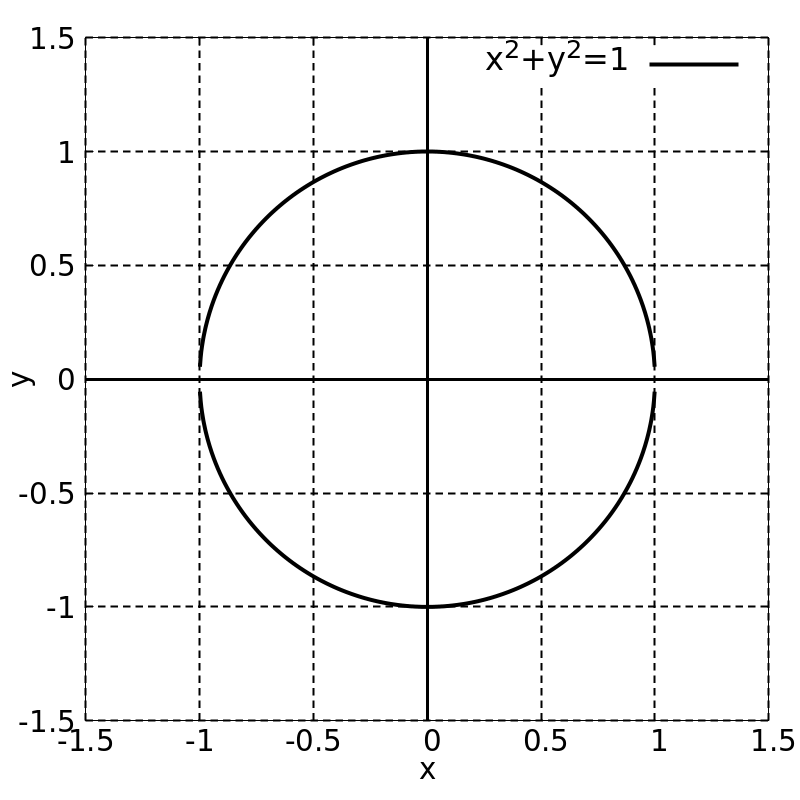
\includegraphics[width=0.45\textwidth]{./gnuplot/implicit-fun-circle}
    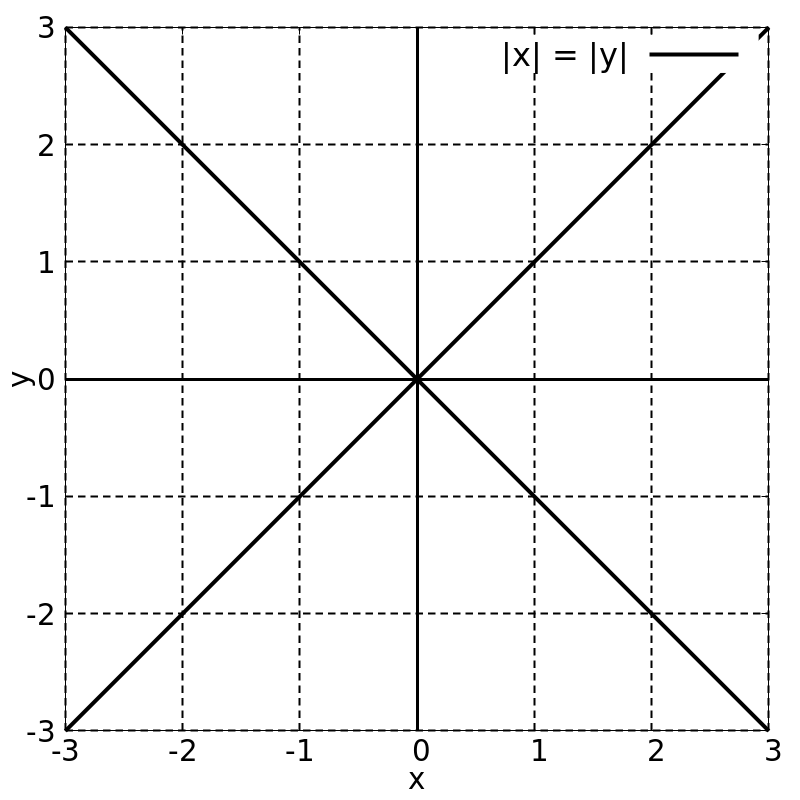
\includegraphics[width=0.45\textwidth]{./gnuplot/implicit-fun-cross}
    \caption{Graphen implizit gegebener Funktionen. Man beachte, dass immer nur ein Teil des Kreises und des Kreuzes als explizite Abbildung von Argumenten nach Funktionswerten aufgefasst werden kann.}
\end{figure}

Neben dem Pfeildiagramm gibt es noch weitere Möglichkeiten, ein- und mehrstellige Funktionen graphisch darzustellen.

\begin{definition}{Graph einer Funktion}{FunGraph}
    Der Graph $G$ einer n-stelligen Funktion $f: \R^n \to \R$ ist die Menge aller $(n+1)$-dimensionalen Punkte, die einem Argument-Funktionswerte-Paar entsprechen.

    $$
    G = \lbrace (p_1, p_2, ..., p_{n+1}) \in R^{n+1} | f((p_1, ..., p_n)) = p_{n+1} \rbrace
    $$

    Dieser Graph kann in einem $(n+1)$-dimensionalen kartesischen Koordinatensystem veranschaulicht werden.
\end{definition}

Ein kleiner Hinweis zum Zeichnen von Graphen. \href{http://www.gnuplot.info/}{gnuplot} ist ein Open-Source-Programm, mit dem man Graphen zeichnen kann, welches auch für die Illustrationen in diesem Skript verwendet wird. \href{http://maxima.sourceforge.net/}{Maxima} und \href{https://www.sagemath.org/}{sage} sind \mention{Cas}-Programme (Computer-Algebra-System), mit denen auch Graphen gezeichnet werden können. Online kann beispielsweise \href{https://www.geogebra.org/graphing}{GeoGebra} oder \href{https://www.wolframalpha.com/examples/mathematics/plotting-and-graphics/}{Wolfram Alpha} genutzt werden.

Für einstellige Funktionen ist der Graph zweidimensional und in einem $x-y$-Koordinatensystem wie in Abbildung \ref{fig:GraphUnivarFun} gut überschaubar. Für zweistellige Funktionen benötigt man bereits ein dreidimensionalen Koordinatensystem, in dem die Form des Graphen bereits schwerer zu überschauen ist, da der Graph meist auf eine zweidimensionale Bildschirmebene projiziert wird. Drei- und mehrstellige Funktionen sind auf diese Weise nur kaum bis gar nicht zur veranschaulichen. Die meisten Beispiele dieser Vorlesung werden sich daher auf ein- und zweidimensionale Funktionen beschränken. In Abbildung \ref{fig:GraphUnivarFun} ist der Graph einer einstelligen Funktion dargestellt. Abbildung \ref{fig:GraphMultivarFun} zeigt den Graph einer zweistelligen Funktion aus vier verschiedenen Blickwinkeln. Man beachte hierbei besonders die Seitensicht: Wird eines der beiden Argumente konstant gehalten und nur das anderen variiert, erhält man eine einstellige Funktion. Je nachdem, auf welchem Wert man das eine Argument konstant hält, ergeben sich verschiedene Funktionen.

\begin{figure}[h]
    \label{fig:GraphUnivarFun}
    \centering
    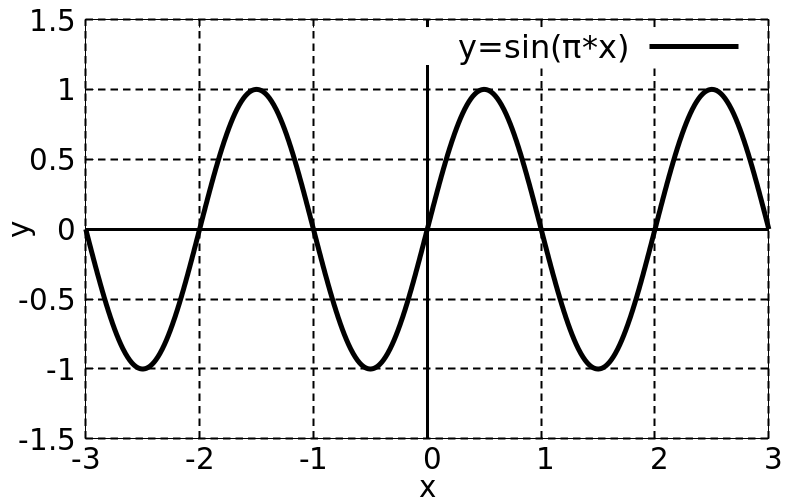
\includegraphics[width=0.8\textwidth]{./gnuplot/example-univariate-function.png}
    \caption{Graph einer einstelligen Funktion}
\end{figure}

\begin{figure}[h]
    \label{fig:GraphMultivarFun}
    \centering
    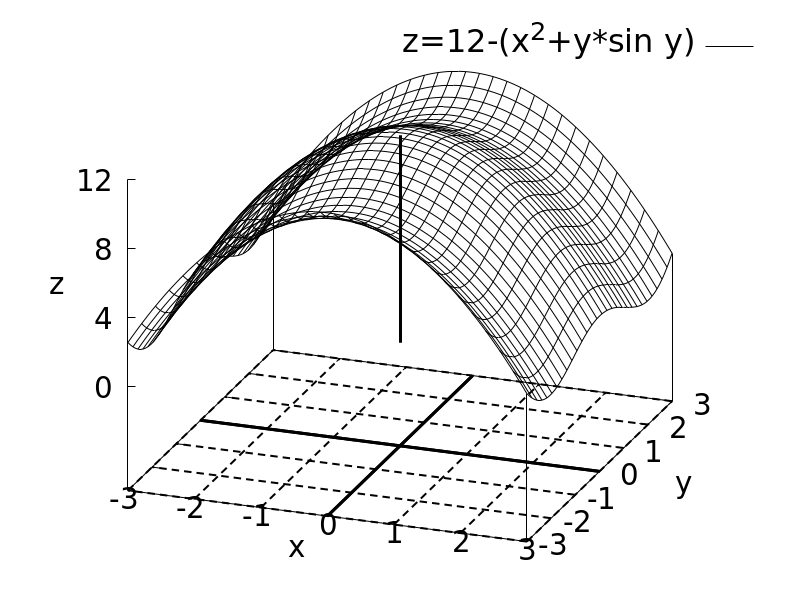
\includegraphics[width=0.45\textwidth]{./gnuplot/example-multivariate-function-1}
    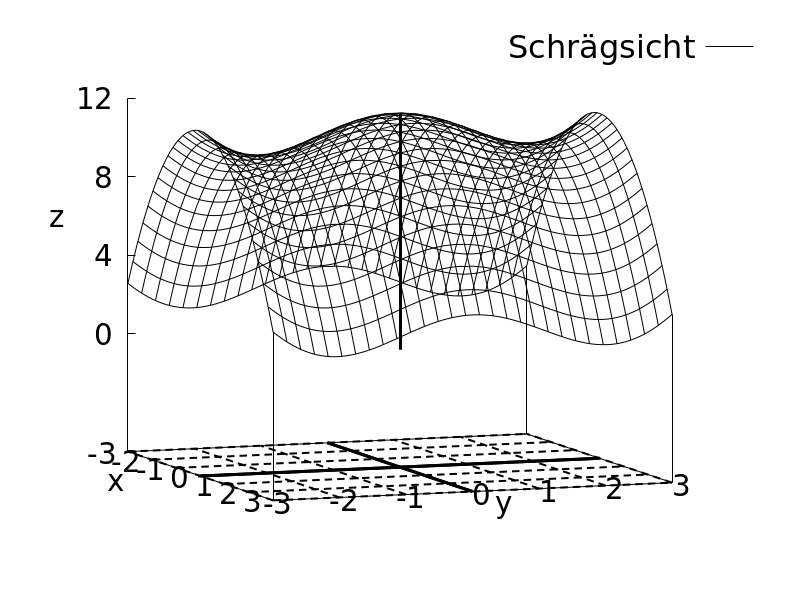
\includegraphics[width=0.45\textwidth]{./gnuplot/example-multivariate-function-2}
    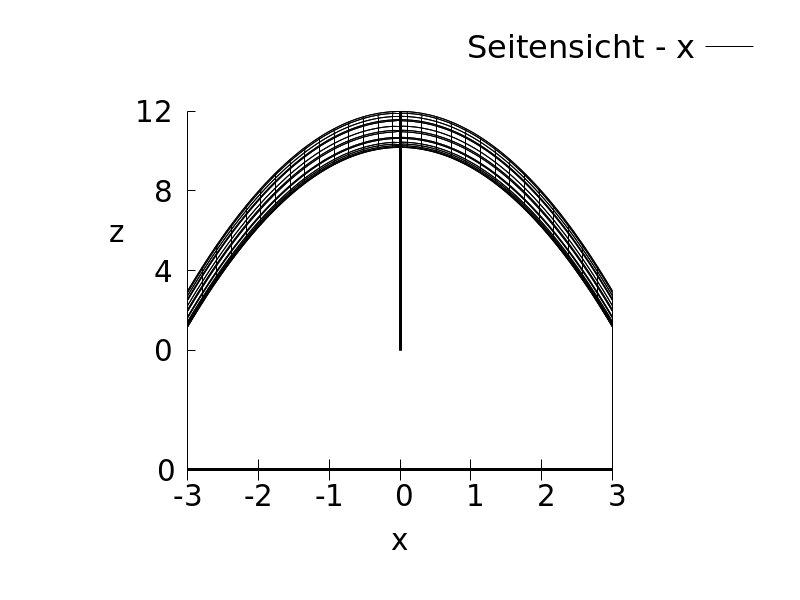
\includegraphics[width=0.45\textwidth]{./gnuplot/example-multivariate-function-3}
    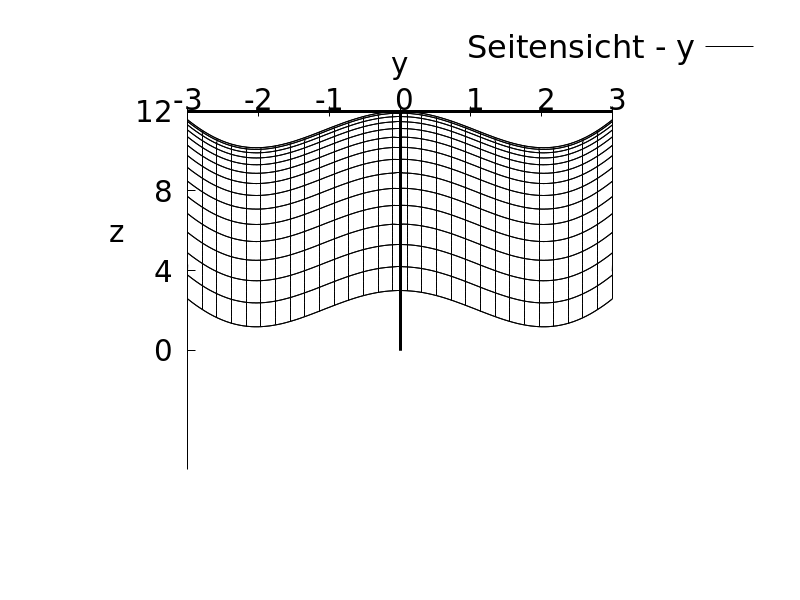
\includegraphics[width=0.45\textwidth]{./gnuplot/example-multivariate-function-4}
    \caption{Graph einer zweistelligen Funktion}
\end{figure}

Für zweistellige Funktionen gibt es auch noch weitere Darstellungsformen, die manchmal übersichtlichen und einfacher zu erfassen sind. Die erste Darstellungsweise, die sogenannte \emph{Konturdarstellung}, wird etwa bei Wanderkarten für Abbildung zweidimensionaler Punkte der Erdoberfläche zur Höhe über Normalnull verwendet. Die Höhe an jedem Punkt wird farbig markiert, Kurven gleicher Höhe werden mit einer Linie dargestellt (Höhenlinien).

\begin{definition}{Konturlinie einer mehrstelligen Funktion}{ContLine}
    Unter einer \textbf{Konturlinie} zur Konstanten $c$ einer n-stelligen Funktion $f: \R^n\to\R$ versteht man die Menge $L_c$ aller Punkte des Definitionsbereichs, an dem der Funktionswert gleich der Konstanten $c$ ist.

    $$
       L_c = \lbrace x \in \R^n | f(x) = c \rbrace
    $$
\end{definition}

\begin{example}{Konturlinien einer Funktion}{ContLine}
    Gesucht sind die Konturlinien der zweistelligen Funktion $f: (x,y) \mapsto x^2+y^2$. Offensichtlich kann die Funktion keine negativen Werte annehmen. Wir bezeichnen die Konturlinienkonstante mit $R^2$. Nach Definition sind nun die Punkte $(x,y)\in\R^2$ gesucht, für die $x^2+y^2=R^2$ gilt. Unter Beachtung des Satzes von Pythagoras erkennen wir, dass es sich um alle Punkte handelt, deren Abstand zum Koordinatenursprung $R$ beträgt. Mithin handelt es sich bei den Konturlinien von $f$ also um zum Ursprung konzentrische Kreislinien. Diese sind in Abbildung \ref{fig:ExContLine} dargestellt.
\end{example}

\begin{figure}[h]
    \label{fig:ExContLine}
    \centering
    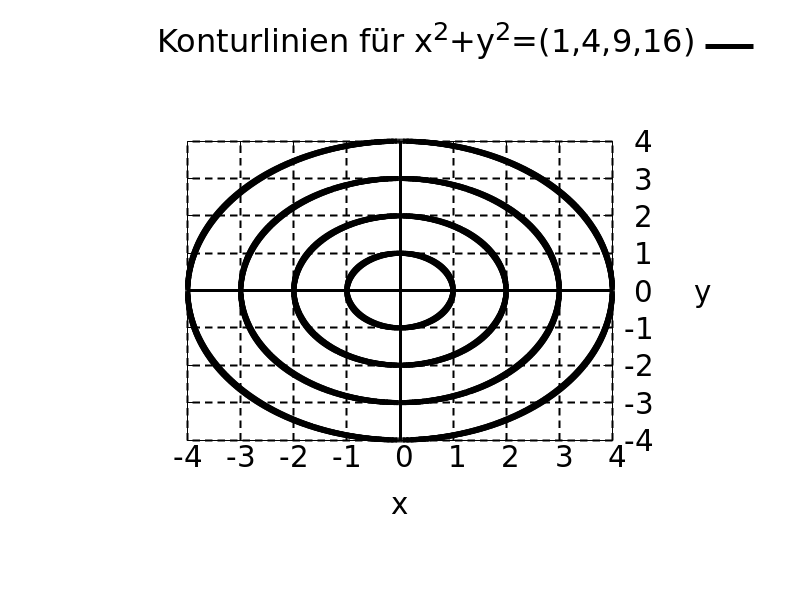
\includegraphics[width=0.6\textwidth]{./gnuplot/example-contour-plot}
    \caption{Konturlinien der Funktion aus Beispiel \ref{ex:ContLine}}
\end{figure}

Ein Beispiel für die Konturlinien mit farbiger Hervorhebung für eine komplexere Funktion findet sich in Abbildung \ref{fig:ContourComplexFun}.

Als zweite Darstellungsform gibt es noch das sogenannte Gradientenfeld, wobei durch Pfeile angezeigt wird, in welcher Richtung die Funktionswerte am stärksten zunehmen. Dies ist etwa bekannt aus Wetterkarten, wo die Windrichtung (näherungsweise) als Gradient des Luftdruckes eingezeichnet ist.

\begin{definition}{Gradientenfeld einer zweistelligen Funktion}{GradField}
    Unter dem Gradientenfeld einer $n$-stelligen Funktion $f: \R^n \to R$ versteht man die Funktion $G_f: \R^n \to \R^n$, welche jedem Punkt $\vec{r}=(x_1,x_2,...,x_n)$ des Definitionsbereichs von $f$ eine Richtung (einen $n$-dimensionalen Vektor) zuordnet, welcher in Richtung des stärksten Anstiegs von $f$ im Punkt $\vec{r}$ zeigt.

    $$
        G_f(\vec{r}) = \vec\nabla f(\vec{r}) = \rvec{\pdd{f}{x_1}(\vec{r})}{\vdots}{\pdd{f}{x_n}(\vec{r})}
    $$
\end{definition}

\begin{example}{Konturlinien einer Funktion}{GradField}
    Gesucht ist das Gradientenfeld der zweistelligen Funktion $f: (x,y) \mapsto x^2+y^2$. Gemäß Definition müssen wir zuerst die beiden partiellen Ableitungen nach $x$ und $y$ berechnen:

    \begin{alignat*}{1}
        \pdd{}{x} x^2+y^2 &= 2x \\
        \pdd{}{y} x^2+y^2 &= 2y
    \end{alignat*}

    Damit lässt sich das Gradientenfeld $G: \R^2 \to \R$ nun angeben als:

    $$
        G(x,y) = \tvec{2x}{2y}
    $$

    Die Richtung des stärksten Anstiegs verläuft wie in Abbildung \ref{fig:ExGradField} zu sehen also immer radial weg vom Koordinatenursprung. Aus der Anschauung ist dies unmittelbar klar, bei dem Graphen von $f$ handelt es sich um einen nach oben geöffnete Kesselform.
\end{example}

\begin{figure}[h]
    \label{fig:ExGradField}
    \centering
    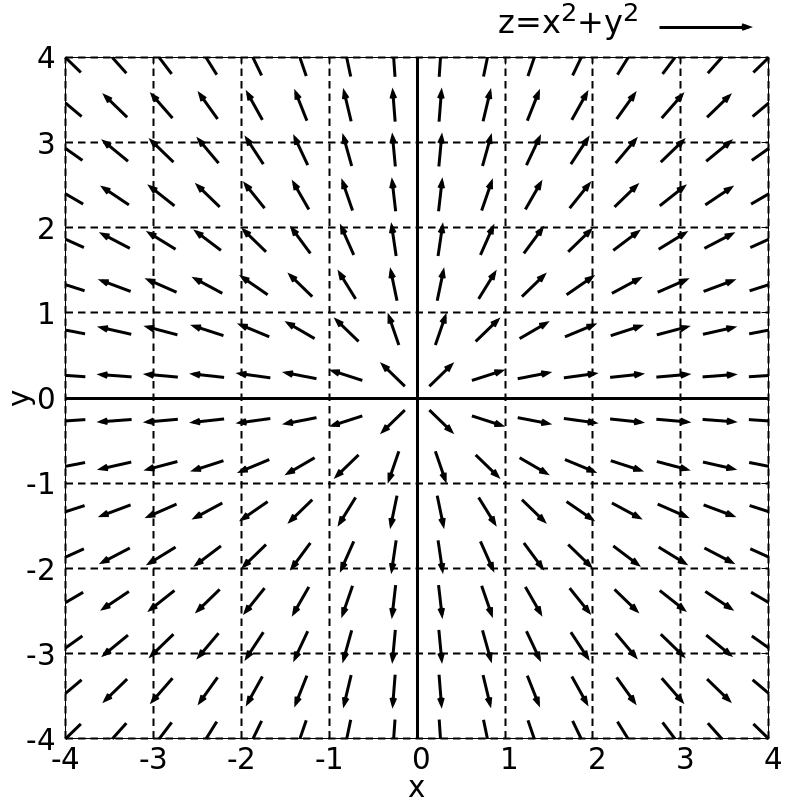
\includegraphics[width=0.65\textwidth]{./gnuplot/example-gradient-field}
    \caption{Gradientenfeld der Funktion aus Beispiel \ref{ex:GradField}}
\end{figure}

An dieser Stelle noch eine kurze Anmerkung zum sogenannten \emph{Feld}. Speziell in der Physik bezeichnet man mit einem Feld eine Größe, welche an jedem Punkt des Raums einen anderen Wert haben kann. Diese stellen mehrstellige Funktionen dar. Etwa ist der Luftdruck ein Feld, wo jedem Raumpunkt ein Luftdruckwert zugeordnet wird. Da der Luftdruck nur ein einzelne Zahl (=Skalar) ist, nennt man solche Felder auch skalare Felder. Das elektrische Feld ist ein vektorielles Feld und weist jedem Raumpunkt einen Vektor (Richtung und Betrag) zu, der angibt, welche Kraft eine geladene Masse an diesem Raumpunkt erfährt.

\section{Transformation von Funktionen}

TODO!!

Transformationen (Verschiebung, Skalierung)
Verkettung

\section{Eigenschaften von Funktionen}

Bisher haben wir Funktionen nur als allgemeine Zuordnung von Elemente einer Menge zu Elementen einer anderen Menge kennengelernt. In der Analyse von und bei der Arbeit mit Funktionen ist es wichtig zu wissen, welche Eigenschaften eine Funktion hat. Im Folgenden werden einige besonders wichtige Eigenschaften von Funktionen besprochen.

\subsection{Umkehrbarkeit}

Mittels einer Funktionsgleichung lässt sich berechnen, welcher Funktionswert zu einem Argument gehört. Für die Praxis ist es oft auch relevant, zu einem gegebenen Funktionswert das zugehörige Argument zu berechnen. In der Analyse von radioaktiven Zerfällen kann man sich etwa fragen, wie lange man warten muss, bis die Strahlungsdosis auf die Hälfte oder auf ein Drittel abgefallen ist. Mathematisch entspricht dies der Umkehrfunktion, welche eine Abbildung von den Funktionswerten zu den Argumenten vermittelt. Nun ist es so, dass nicht jede Funktion umkehrbar ist. Um beschreiben zu können, wann dies möglich ist, müssen wir zuerst die Begriffe \emph{Injektivität} und \emph{Surjektivität} einer Funktion definieren. Dies werden wir allgemeingültig für alle Funktionen tun, nicht nur für reellwertige oder einstellige Funktionen.

\begin{definition}{Injektivität einer Funktion}{Injective}
    Sei $f: \mathbb{D} \to \mathbb{C}$ eine Funktion mit Definitionsbereich $\mathbb{D}$ und Wertebereich $\mathbb{C}$. $f$ heißt \textbf{injektiv}, wenn eine Funktion $g: \mathbb{C} \to \mathbb{D}$ existiert mit der Eigenschaft:
    $$
    g \circ f = \mathbbm{1}_\mathbb{D}
    $$
    Äquivalent dazu ist die Forderung, dass kein Funktionswert doppelt angenommen wird, sich also gleiche Funktionswerte nur aus gleichen Argumenten ergeben: $\forall x_1,x_2\in\mathbb{D}: f(x_1)=f(x_2) \implies x_1=x_2$.
\end{definition}

\begin{definition}{Surjektivität einer Funktion}{Surjective}
    Sei $f: \mathbb{D} \to \mathbb{C}$ eine Funktion mit Definitionsbereich $\mathbb{D}$ und Wertebereich $\mathbb{C}$. $f$ heißt \textbf{surjektiv}, wenn eine Funktion $g: \mathbb{C} \to \mathbb{D}$ existiert mit der Eigenschaft:
    $$
    f \circ g = \mathbbm{1}_\mathbb{C}
    $$
    Äquivalent dazu ist die Forderung, dass jeder Funktionswert wenigstens einem Argument zugeordnet ist, dass also $f(\mathbb{D}) = \mathbb{C}$ gilt. Dabei bezeichnet $f(\mathbb{D})$ die Menge aller Elemente, die man erhält wenn man auf jedes Argument die Funktion anwendet.
\end{definition}

Anhand dieser beiden Definitionen können wir nun ein Kriterium dafür angeben, wann die Umkehrfunktion zu einer Funktion existiert.

\begin{statement}{Umkehrbarkeit einer Funktion}{InverseFun}
    Sei $f: \mathbb{D} \to \mathbb{C}$ eine Funktion mit Definitionsbereich $\mathbb{D}$ und Wertebereich $\mathbb{C}$. $f$ heißt \textbf{bijektiv}, wenn $f$ sowohl injektiv als auch surjektiv ist. Dann existiert genau eine Funktion $f^{-1}: \mathbb{C} \to \mathbb{D}$, welche die Bedingungen für Injektivität und Surjektivität erfüllt:
    $$
    f^{-1} \circ f = \mathbbm{1}_\mathbb{D}, f \circ f^{-1} = \mathbbm{1}_\mathbb{C}
    $$
    Es heißt dann $f^{-1}$ die \textbf{Umkehrfunktion} zu $f$.
\end{statement}

Bezüglich der Notation beachte man, dass $f^{-1}$ nicht das Reziproke $\frac{1}{f}$ bezeichnet, sondern nur eine symbolische Schreibweise für die Umkehrfunktion ist. Sie leitet sich darauf ab, dass die Hyperbelfunktion $x \mapsto 1/x$ die Umkehrfunktion zur linearen Funktion $x \mapsto x$ ist.

Rechnerisch erhält man die Umkehrfunktion aus der Funktionsgleichung $y = f(x)$, indem man diese nach $x = f^{-1}(y)$ umstellt. Man vertauscht dabei also $x$ und $y$. Graphisch entspricht das Bilden der Umkehrfunktion der Spiegelung an der Hauptgeraden $y=x$.

\begin{figure}[h]
    \label{fig:InjectSurject}
    \centering
    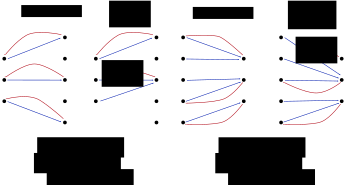
\includegraphics[width=0.95\textwidth]{./svg/injective-surjective}
    \caption{Graphische Darstellung der Definition von Injektivität und Surjektivität. Es ist jeweils eine Beispiel für eine Abbildung dargestellt, welche die Bedingung erfüllt, und ein Beispiel, wo sie die Bedingung nicht erfüllt. Die Bedingung, dass sich die Identitätsfunktion ergeben soll, bedeutet graphisch, dass man an einem Punkt anfängt, den Pfeilen folgt, und schließlich wieder am Ausgangspunkt ankommt. Das ist bei dem nicht-injektiven beziehungsweise nicht-surjektiven Beispiel nicht möglich.}
\end{figure}

\begin{example}{}{}
    \begin{enumerate}
        \item Die Funktion $f: (-\infty,\infty) \to (-\infty,\infty)$ mit $x \mapsto x^2$ ist nicht surjektiv, denn es kann keine Abbildung $g: (-\infty,\infty) \to (-\infty,\infty)$ geben. Für diese müsste etwa auch $(f \circ g)(-1) = g(-1)^2 = -1$ gelten, was aber nicht möglich ist, da bei der Quadratbildung nur nichtnegative Werte möglich sind. Durch Einschränkung des Wertebereichs kann dieses Problem wie im nächsten Beispiel illustriert gelöst werden.
        \item Die Funktion $f: (-\infty,\infty) \to [0,\infty)$ mit $x \mapsto x^2$ ist surjektiv, aber nicht injektiv. Sie ist surjektiv, da etwa die Funktion $g: [0,\infty) \to (-\infty,\infty)$ mit $x \mapsto \sqrt{x}$ existiert,  sodass gilt $(f \circ g)(x) = (\sqrt{x})^2 = x$. Die Funktion ist nicht eindeutig, genauso hätten wir $g: x \mapsto -\sqrt{x}$ wählen können, auch hier gilt $(-\sqrt{x})^2 = x$. Allerdings ist $f$ nicht injektiv, für beide Kandidaten einer Umkehrfunktion ist $(g \circ f)(x) = \pm\sqrt{x^2} = \pm|x| \ne x$. Durch Einschränkung des Definitionsbereichs auch wie im nächsten Beispiel auch dieses Problem umgangen werden.
        \item Die Funktion $f: (0,\infty) \to [0,\infty)$ mit $x \mapsto x^2$ ist injektiv. Es existiert die Funktion $g: x \mapsto \sqrt{x}$, sodass gilt: $\sqrt{x^2}=|x|=x$ (da $x\ge 0$). Zudem gilt auch $\left(\sqrt{x}\right)^2=x$, $f$ ist also surjektiv. Mithin ist $f$ bijektiv, es existiert die Umkehrfunktion $f^{-1}(x) = \sqrt{x}$, welche den rechten Parabelast darstellt.
        \item Die Funktion $f: (-\infty,0] \to [0,\infty)$ mit $x \mapsto x^2$ ist ebenso umkehrbar. Es existiert die Funktion $g: x \mapsto -\sqrt{x}$, sodass gilt: $-\sqrt{x^2}=-|x|=x$ (da $x\le 0$). Die Umkehrfunktion lautet $f^{-1}(x) = -\sqrt{x}$, welche den linken Parabelast darstellt.
        \item Die Funktion $f: (-\infty,\infty) \to (0, \infty)$ mit $x \mapsto e^x$ ist umkehrbar. Die Funktion $f^{-1}: (0, \infty) \to (-\infty,\infty)$ mit $x \mapsto \ln(x)$ erfüllt die Eigenschaften für die Injektivität und die Surjektivität, da gilt: $e^{\ln(x)} = \ln(e^x) = x$.  Mithin ist $\ln(x)$ die Umkehrfunktion zu $e^x$.
    \end{enumerate}
\end{example}

\subsection{Monotonie}

Eine Funktion kann auch daraufhin untersucht werden, ob ihr Graph beständig ansteigt oder abfällt. Wir wollen uns hier auf einstellige Funktionen beschränken, für mehrstellige Funktionen kann es passieren, dass die Funktionswerte in eine Richtung fallen und in einer anderen Richtung steigen.

\begin{definition}{Monotonie einer einstelligen Funktionen}{UnivarMonotonic}
    Eine einstellige, reellwertige Funktion $f: \R \to \R$ heißt in einem offenen Interval $U\subset\R$ \textbf{monoton steigend} (\textbf{fallend}), wenn größere Argumente immer gleiche oder größere (kleinere) Funktionswerte zur Folge haben, falls also gilt:
    $$
        \forall x_1,x_2 \in U: x_2 > x_1 \implies f(x_2) \ge f(x_1)
    $$
    $$
      ( \forall x_1,x_2 \in U: x_2 > x_1 \implies f(x_2) \le f(x_1) )
    $$
    Gilt auf der rechten Seite der Implikation sogar einer Größer-Zeichen (Kleiner-Zeichen), heißt die Funktion \textbf{streng monoton steigend} (\textbf{streng monoton fallend}).
\end{definition}

Wenn eine Funktion auf ihrem gesamten Definitionsbereich monoton ist, heißt sie monoton steigende oder fallende Funktion. Ansonsten unterteilt man den Definitionsbereich in Teilmengen und untersucht dort auf Monotonie.

\begin{example}{Untersuchung auf Monotonie}{ExamMonot}
    \begin{enumerate}
        \item Die lineare Funktion $x \mapsto 3x$ ist streng monoton steigend, denn aus $x_2 > x_1$ folgt $3x_2^2 > 3x_1^2$.
        \item Die quadratische Funktion $x \mapsto x^2$ ist nur auf Teilbereichen monoton. Für $x\le 0$ ist sie streng monoton fallend, denn aus $x_2 > x_1$ folgt für negative Werte $x_2^2 < x_1^2$. Analog ist sie für $x\ge 0$ streng monoton steigend.
        \item Die Sinusfunktion $x \mapsto \sin(x)$ ist $x\in[\degrees{0},\degrees{90}]$ streng monoton steigend, für $x\in[\degrees{90}, \degrees{0},270]$ streng monoton fallend und für $x\in[\degrees{270},\degrees{360}]$ wieder streng monoton steigend.
        \item Die konstante Funktion $x \mapsto 42$ ist sowohl monoton steigend als auch monoton fallend, aber nicht streng monoton steigend oder fallend.
    \end{enumerate}
\end{example}

\subsection{Symmetrie}

Ein weiteres wichtiges Merkmal einer Funktion ist ihr sogenanntes Symmetrieverhalten. Dieses gibt an, wie sich der Funktionswert ändert, wenn das Argument negiert wird, also beispielsweise $-3$ statt $3$ in die Funktionsgleichung eingesetzt wird. Man unterscheidet zwei wesentliche Fälle:

\begin{definition}{Symmetrie einer einstelligen Funktionen}{UnivarSymm}
    Sei $f: \R \to \R$ eine einstellige, reellwertige Funktion.

    $f$ heißt \textbf{achsensymmetrisch} oder \textbf{gerade} Funktion, wenn ihr Funktionswert sich unter Negation des Arguments nicht ändern, falls also für alle Argumente gilt: $f(x) = f(-x)$.

    $f$ heißt \textbf{punktsymmetrisch} oder \textbf{ungerade} Funktion, wenn ihr Funktionswert sich unter Negation des Arguments ebenfalls negiert, aber betragsmäßig gleich bleibt, falls also für alle Argumente gilt: $f(x) = -f(-x)$.
\end{definition}

Man beachte hierbei, dass die Wahl der Begriffe \emph{achsensymmetrisch} und \emph{punktsymmetrisch} nicht willkürlich gewählt sind. Man überlegt sich schnell, dass achsensymmetrische Funktionen tatsächlich symmetrisch bezüglich der vertikalen Spiegelachse $x=0$ sind. Ebenso sind punktsymmetrische Funktionen punktsymmetrisch zum Punkt $(0,0)$.

\begin{example}{Untersuchung auf Symmetrie}{ExamSymm}
    \begin{itemize}
        \item Die Funktion $x \mapsto x^2$ ist eine gerade Funktion, denn es gilt $f(-x) = (-x)^2 = (-1)^2 x^2 = x^2 = f(x)$.
        \item Die Funktion $x \mapsto x^3$ ist eine ungerade Funktion, denn es gilt $f(-x) = (-x)^3 = (-1)^3 x^3 = -x^3 = -f(x)$.
    \end{itemize}
\end{example}

\begin{figure}[h]
    \label{fig:ExAxisSymFun}
    \centering
    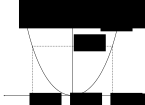
\includegraphics[width=0.45\textwidth]{./svg/axis-symmetric-fun}
    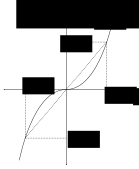
\includegraphics[width=0.45\textwidth]{./svg/point-symmetric-fun}
    \caption{Links: Achsensymmetrische Funktion. Der rechte Teile der Parabel geht unter Spiegelung an der Ordinate in den linken Teil über. Rechts: Punktsymmetrische Funktion: Der rechte Teil der kubischen Parabel geht unter Punktspiegelung am Ursprung in den linken Teil über.}
\end{figure}

Von besonderer Bedeutung sind diese beiden Symmetrieeigenschaften, da sich alle Funktionen, sofern sie denn für positive und negative Argumente überhaupt definiert sind, zerlegen lassen in die Summe aus einem geraden und einem ungerade Anteil.

\begin{statement}{Gerader und ungerade Anteil einer Funktion}{SplitEvenOddFun}
    Sei $f: \R \to \R$ eine einstellige reellwertige Funktion mit einem Definitionsbereich $\mathbb{D}$ derart, dass $x\in\mathbb{R} \iff -x\in\mathbb{D}$ gilt, also zu jedem Argument auch sein Negiertes zum Definitionsbereich gehört. Seien weiterhin $e$ und $o$ wie folgt definierte Funktionen:

    \begin{alignat*}{1}
        e(x) &= \frac{f(x) + f(-x)}{2} \\
        o(x) &= \frac{f(x) - f(-x)}{2}
    \end{alignat*}

    Dann ist $e$ eine gerade (\emph{event}) Funktion und $o$ eine ungerade (\emph{odd}) Funktion; und es gilt: $f(x) = e(x) + o(x)$.
\end{statement}

Dass die Funktionen $e$ und $o$ gerade beziehungsweise ungerade sind, zeigt man leicht anhand der Definition. Durch Aufaddieren beider Funktionen und Zusammenfassen des Bruches zeigt man, dass man so die ursprüngliche Funktion $f$ erhält. Dieser Zerlegung kommt unter anderem deswegen Bedeutung zu, weil sie eine Definition der trigonometrischen und hyperbolischen Funktionen über die Exponentialfunktion erlaubt, wie wir im nächsten Abschnitt zu speziellen Funktionen sehen werden.

\begin{example}{Emittlung des geraden und ungeraden Anteils einer Funktion}{CompEvenOddPart}
    Gesucht ist der gerade und ungerade Anteil von $x \mapsto x^2+x^3$. Nach Aussage \ref{stmt:SplitEvenOddFun} berechnen wir $e(x) = \frac{(x^2+x^3)+((-x)^2)+(-x)^3)}{2} = \frac{x^2+x^3+x^2-x^3}{2} = x^2$ und $o(x) = \frac{(x^2+x^3)-((-x)^2)+(-x)^3)}{2} = \frac{x^2+x^3-x^2+x^3}{2} = x^3$. Dies ist deshalb nicht überraschend, da wir bereits wissen, dass $x\mapsto x^2$ gerade und $x \mapsto x^3$ ungerade ist.
\end{example}

\subsection{Periodizität}

Die Periodizität ist eine Eigenschaft von periodischen Funktionen, deren Funktionswerte sich nach einer bestimmten Periode immer wiederholen. Die Sinus- und Kosinusfunktionen sind ein bekanntes Beispiel für periodische Funktionen.

\begin{definition}{Periode einer einstelligen Funktion}{PeriodUnivarFun}
    Sei $f: \R \to \R$ eine einstellige reellwertige Funktion mit Definitionsbereich $\mathbb{D}$. $f$ heißt \textbf{periodisch}, wenn es eine reelle Zahl $p>0$ gibt, sodass gilt:
    $$
        \forall x \in \mathbb{D}: f(x) = f(x+p)
    $$
    Jede solche Zahl $p$ heißt dann \textbf{Periode}. Die kleinste solche Zahl $p$ nennt man \textbf{primitive Periode} der Funktion.
\end{definition}

Aus dieser Definition erkennt man sofort, dass wenn $p$ eine Periode der Funktion ist, auch $2p$ eine Periode ist: per Definition gilt $f(x) = f(x+p)$ und $f(x+p)=f(x+p+p)=f(x+2p)$, mithin also auch $f(x) = f(x+2p)$. Allgemein ist jedes ganzzahlige Vielfache der primitiven Periode auch eine Periode. Oft wird statt dem Begriff \emph{primitive Periode} auch einfach nur \emph{Periode} verwendet.

\begin{example}{Untersuchung der Periodizität}{ExamPeriod}
    \begin{enumerate}
        \item Die Funktion $x \mapsto \tan(x)$ ist periodisch, denn beispielsweise ist $p=2\pi$ eine Periode, da $\tan(x+2\pi)=\frac{\sin(x+2\pi)}{\cos(x+2\pi)} = \frac{\sin(x)}{\cos(x)} = \tan(x)$ gilt. Die kleinste Periode ist $p=\pi$ (=$\degrees{180}$) und stell damit die primitive Periode der Tangensfunktion dar.
        \item Auch die konstante Funktion $x \mapsto 42$ ist periodisch. Jedes $p>0$ ist eine Periode der Funktion. Allerdings gibt es keine kleinste Periode (da $p=0$ per Definition ausgeschlossen ist).
    \end{enumerate}
\end{example}


Stetigkeit, stetige Erägnzung

Verhalten im Unendlichen


Nulstelle, y-AchsenSchnittpkt. Polstelle sprungstelle

Globale Extreme, Lokale Extrema

\section{Spezielle Funktionen}

In diesem Abschnitt betrachten wir zuerst einige grundlegende Funktionen und schauen uns dann an, wie komplexere Funktionen durch Kombination von anderen Funktionen gewonnen werden können.

\begin{minipage}[t]{1\textwidth}
    \begin{wrapfigure}{L}{6cm}
        \label{fig:ExBaseFunLin}
        \centering
        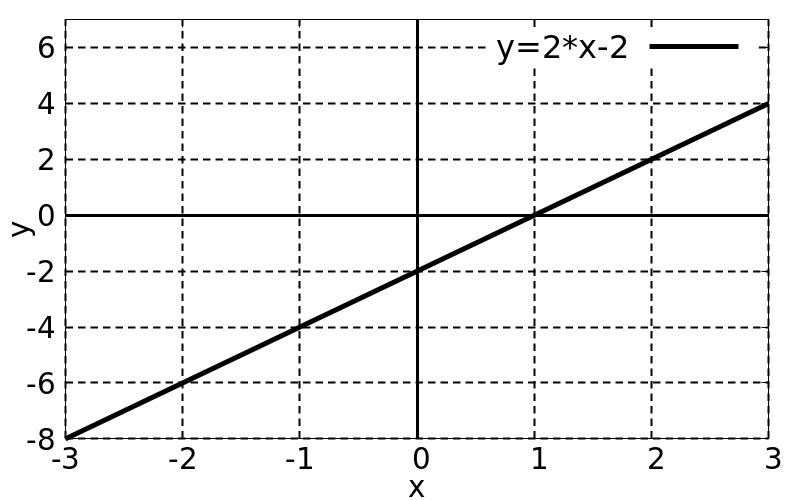
\includegraphics[width=6cm]{./gnuplot/base-function-linear}
        \caption{Graph einer linearen Funktion}
    \end{wrapfigure}
    \textbf{Lineare Funktionen} beschreiben ein konstantes Wachstum oder ein konstantes Gefälle und haben eine \textbf{Gerade} als Graphen. In der Darstellung $x \to mx+n, m\ne 0$ werden sie charakterisiert durch 2 wesentliche Parameter. Der Anstieg $m$ gibt an, um wieviel der Funktionswert zu- oder abnimmt, wenn das Argument um eine Einheit erhöht wird. Der Startwert $n$ gibt, welcher initiale Funktionswert dem Argument $0$ zugeordnet ist und ist gleichzeitig der Schnittpunkt mit der Ordinate. Lineare Funktionen sind definiert für alle reellen Zahlen und können alle reellen Werte annehmen. Lineare Funktionen werden auch verwendet, um zwischen zwei Punkten $(x_1,y_1)$ und ($x_2,y_2)$ zu interpolieren. Die Gerade, welche durch diese beiden Punkte verläuft, lautet dann $x \to y_1 + \frac{x-x1}{x_2-x_1} \cdot (y_2-y_1)$.
\end{minipage}

\begin{minipage}[t]{1\textwidth}
    \begin{wrapfigure}{R}{6cm}
        \label{fig:ExBaseFunHyperbola}
        \centering
        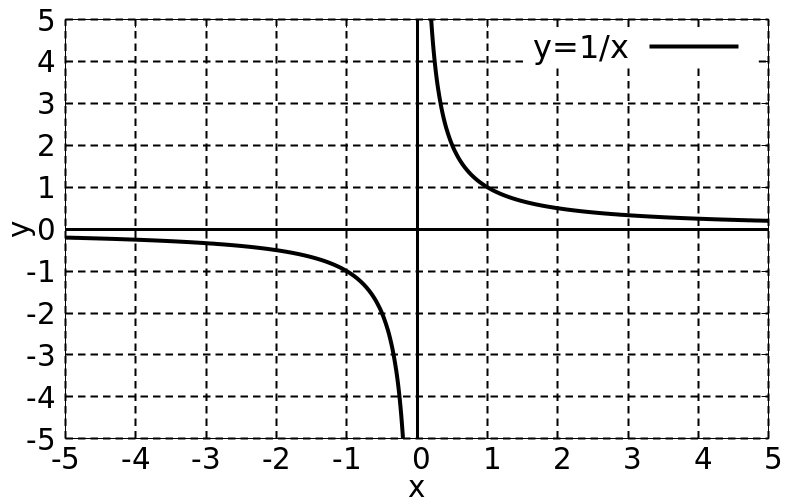
\includegraphics[width=6cm]{./gnuplot/base-function-hyperbola}
        \caption{Graph einer Hyperbelfunktion}
    \end{wrapfigure}
    Die \textbf{Hyperbel} ist der Graph von Funktionen der Form $x \to \frac{a}{x}$. Solche Funktionen beschreiben indirekt proportionale Zusammenhänge, wobei das Verdoppeln des Arguments in einer Halbierung des Funktionswerts resultiert. Aufgrund der Tatsache, dass eine Division durch $0$ nicht erklärt ist, muss diese Zahl auch vom Definitionsbereich ausgeschlossen werden. Zudem ist die $0$ auch nicht für den Wertebereich möglich. Wenn das Argument sich $0$ nähert, wächst der Funktionswert über alle Grenzen, es liegt eine Polstelle vor. Dabei ist es entscheiden, ob man sich von links oder von rechts der Polstelle nähert: $\lim\limits_{n\to 0^-} 1/x = -\infty$, $\lim\limits_{n\to 0^+} 1/x = +\infty$ Für betragsmäßig große Werte nähert sich der Funktionswert $0$, es gilt also $\lim\limits_{x\to\pm\infty} 1/x = 0$.
\end{minipage}

\begin{minipage}[t]{1\textwidth}
    \begin{wrapfigure}{L}{6cm}
        \label{fig:ExBaseFunQuad}
        \centering
        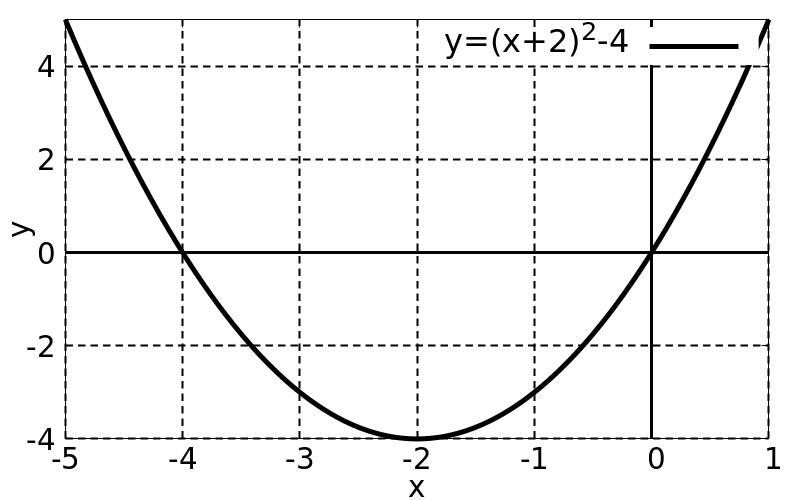
\includegraphics[width=6cm]{./gnuplot/base-function-quadratic}
        \caption{Graph einer quadratischen Funktion}
    \end{wrapfigure}
    \textbf{Quadratische Funktionen} ergeben in der graphischen Darstellung eine \textbf{Parabel}. In der Form $x \to a(x-x_0)^2+y_0, a\ne 0$ wird diese beschrieben durch ihren Scheitelpunkt, der bei $(x_0,y_0)$ liegt, und ihre Krümmung, die durch $a$ beschrieben wird. Für $a<0$ ist die Parabel nach unten geöffnet, für $a>0$ ist sie nach oben geöffnet. Quadratische Funktionen sind für alle reellen Werte definiert. Ihre Wertebereich ist nach oben ($a<0$) beziehungsweise nach unten ($a>0$) durch den Scheitelpunkt beschränkt. Sie sind zudem achsensymmetrisch zur vertikalen Spiegelachse durch den Scheitelpunkt. Physikalisch beschreiben Parabeln unter Anderem Verläufe von Größen, deren Zuwachs oder Abfall konstant ist. Etwa nimmt bei einer gleichmäßigen Beschleunigung die Geschwindigkeit konstant zu oder ab.
\end{minipage}

\begin{minipage}[t]{1\textwidth}
    \begin{wrapfigure}{R}{6cm}
        \label{fig:ExBaseFunRoot}
        \centering
        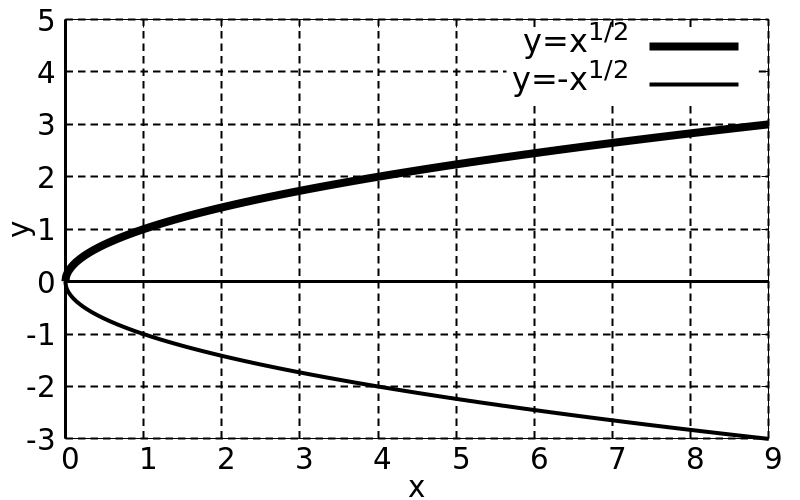
\includegraphics[width=6cm]{./gnuplot/base-function-root}
        \caption{Graph zweier Wurzelfunktionen}
    \end{wrapfigure}
    \textbf{Wurzelfunktionen} $x \to \sqrt{x}$ sind die Umkehrung quadratischer Funktionen, deren Graph eine \textbf{gekippte Parabel} darstellt. Da eine Parabel manche Funktionswerte doppelt annimmt, muss bei der Umkehrung der Definitionsbereich auf den linken oder rechten Parabelast eingeschränkt werden. Links in der Abbildung sind zwei Funktionen dargestellt, zusammen ergeben sie eine vollständige Parabel. Der Definitionsbereich von Wurzelfunktionen ist dadurch beschränkt, dass im Argument der Wurzel nur nichtnegative Argument stehen dürfen. Auch der Wertebereich ist eingeschränkt, da die Wurzeloperation keine negativen Werte zurückliefern kann.
\end{minipage}

\begin{minipage}[t]{1\textwidth}
    \begin{wrapfigure}{L}{6cm}
        \label{fig:ExBaseFunExpo}
        \centering
        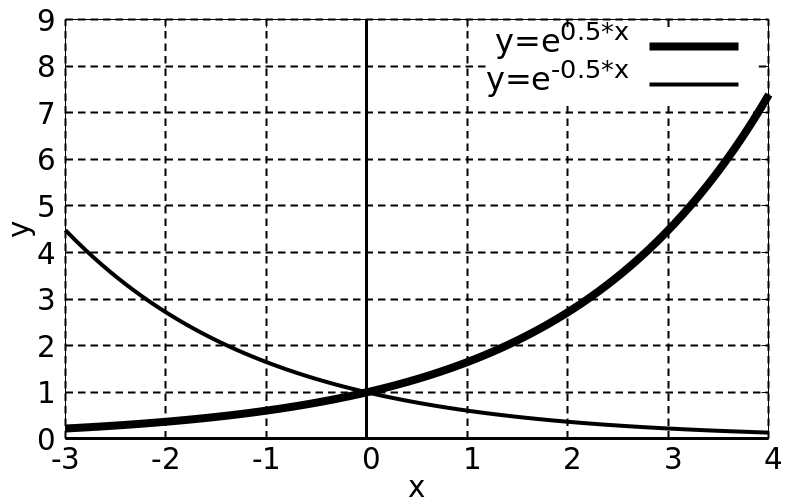
\includegraphics[width=6cm]{./gnuplot/base-function-expo}
        \caption{Graph einer Exponentialfunktion}
    \end{wrapfigure}
    \textbf{Exponentialfunktionen} beschreiben ein exponentielles Wachstum, welches sich etwa in der Zinseszinsrechnung findet, bei radioaktiven Zerfällen eine Rolle spielt oder auch die der Vermehrung von Bakterienkulturen beschreibt. In der Form $x \to a^x, a>0$ stellt der Parameter $a$ ein Maß für den Zuwachs ($a>1$) oder Abfall ($0<a<1$) dar. Etwa bedeutet $x \to 3^x$, dass ein Größe $x$ sich verdreifacht, wenn das Argument $x$ um eine Einheit größer wird. Oft werden Exponentialfunktionen auch mit der Basis $e$ (\mention{Eulersche Zahl}) geschrieben. Dies ist aufgrund der Umformung $a^x = e^{\ln(a)x}$ immer möglich. Exponentialfunktionen sind für alle reellen Zahlen definiert, ihr Wertebereich aber ist dadurch eingeschränkt, dass das Potenzieren nur positive Zahlen liefert. Das Verhalten im Unendlichen hängt vom Parameter $a$ ab. Für den Fall $0<a<1$ näheren sich die Funktionswerte der $0$ für kleine Argumente und steigen unbegrenzt an für große Argumente. Umgedreht verhält es sich für $a>1$. Es gilt $\lim\limits_{x\to-\infty} a^x = \begin{cases} \infty & a \in (0,1)  \\ 0 & a \in (1, \infty) \end{cases}$ und $\lim\limits_{x\to\infty} a^x = \begin{cases} 0 & a \in (0,1)  \\ \infty & a \in (1, \infty) \end{cases}$.
\end{minipage}

\begin{minipage}[t]{1\textwidth}
    \begin{wrapfigure}{R}{6cm}
        \label{fig:ExBaseFunLog}
        \centering
        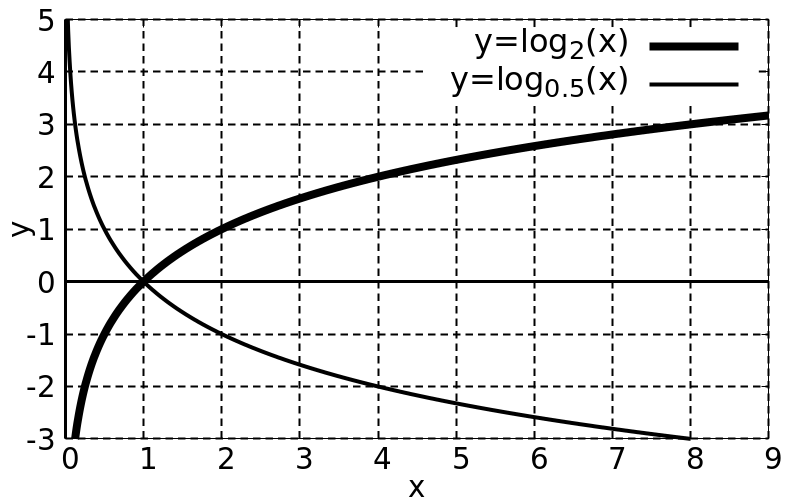
\includegraphics[width=6cm]{./gnuplot/base-function-log}
        \caption{Graph zweier logarithmischer Funktionen}
    \end{wrapfigure}
    \textbf{Logarithmische Funktionen} sind die Umkehrung von Exponentialfunktionen und haben entsprechend ähnliche Eigenschaften. Da das Potenzieren nur positive Zahlen liefert, dürfen im Argument des Logarithmus ebenfalls nur positive Zahlen stehen. Da die Exponentialfunktion beliebige Argument erlaubt, ist der Wertebereich der logarithmischer Funktionen unbeschränkt. In der Form $x \to \log_a{x}$ stellt der Parameter $a$ die Basis des Logarithmus dar, welche ein Maß für die Krümmung der Kurve ist. Für $a>1$ ist die Logarithmusfunktion steigend, für $0<a<1$ fallend. Oft wird sie analog zu Exponentialfunktionen auch mit der Basis $e$ geschrieben, was ebenfalls aufgrund der Umformung $\log_a(x) = \frac{\ln x}{\ln a}$ immer möglich ist. Eine Anwendung von Logarithmen sind sogenannte logarithmische Skalen, die etwa bei der Einheit \emph{Dezibel} oder bei der logarithmischen Achseneinteilung eines Diagramms (siehe \ref{fig:LogScalePlot} und \ref{fig:UniLogScale}) verwendet wird.
\end{minipage}

\begin{minipage}[t]{1\textwidth}
    \begin{wrapfigure}{L}{7cm}
        \label{fig:ExBaseFunExpo}
        \centering
        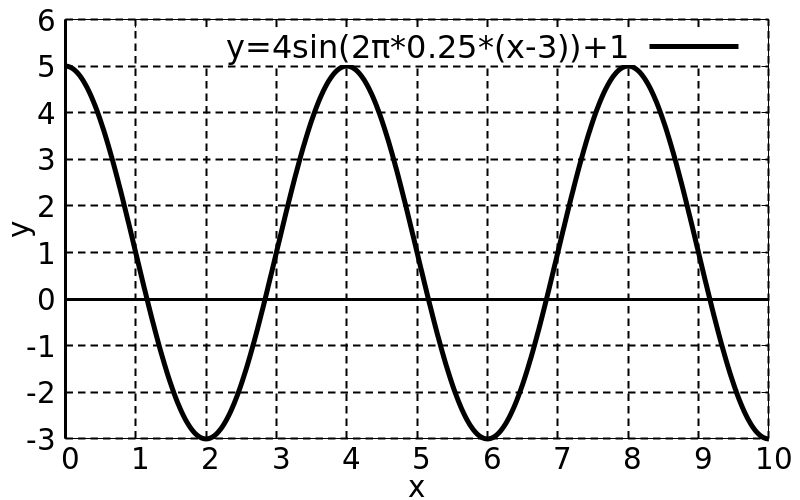
\includegraphics[width=7cm]{./gnuplot/base-function-sine}
        \caption{Graph einer Sinusfunktion}
    \end{wrapfigure}
    \textbf{Trigonometrische Funktionen} (Winkelfunktion) beschreiben Zusammenhänge am Kreis und Dreieck (Verhältnis von An- bzw. Gegenkathete und Abszisse) und in der Physik sogenannte harmonische Schwingungen. Es handelt sich um periodische Funktionen mit beschränktem Wertebereich. In der Form $x \to A\sin(2 \pi f (x-p)) + R$ wird die Schwingung durch vier wesentliche Parameter beschrieben. $R$ gibt die Ruhelage an, um welche sich die Schwingung vollzieht. $A$ bezeichnet die Amplitude, welche die maximale Auslenkung aus der Ruhelage angibt. Der Parameter $f$ stellt die Frequenz der Schwingung dar und ist ein Maß dafür, wieviele Perioden (Schwingungen) in einer Einheit des Arguments $x$ vollzogen werden. Daraus abgeleitet wird auch häufig die sogenannte Kreisfrequenz $w=2\pi f$ und die Periodendauer $T = 1 / f$ verwendet. Schließlich beschreibt $p$ die Phase der Schwingung, also zu welchem Zeitpunkt die Ruhelage durchlaufen wird. Durch Ändern der Phase wird der Graph nach links oder rechts verschoben, dadurch lässt sich eine Sinusfunktion und eine Kosinusfunktion ineinander transformieren. Die Phase spielt eine entscheidende Rolle bei dem physikalischen Phänomenen \emph{Interferenz}.
\end{minipage}

\begin{minipage}[t]{1\textwidth}
    \begin{wrapfigure}{R}{7cm}
        \label{fig:ExBaseFunTan}
        \centering
        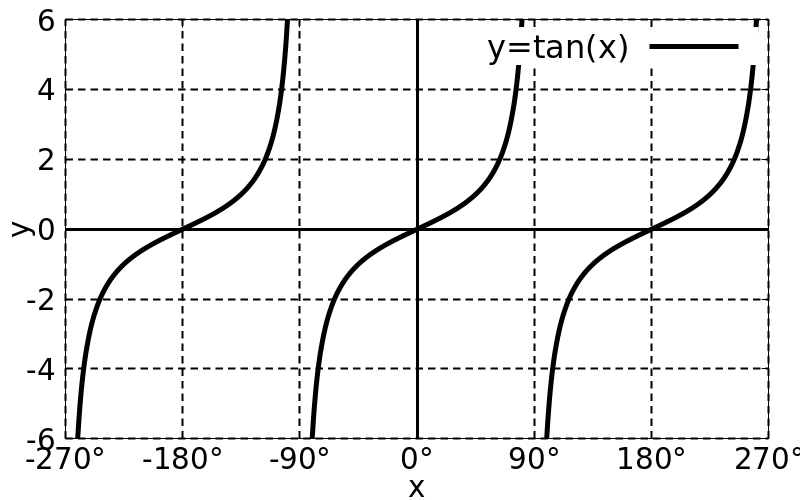
\includegraphics[width=7cm]{./gnuplot/base-function-tan}
        \caption{Graph der Tangensfunktion}
    \end{wrapfigure}
    Die \textbf{Tangensfunktion} ist eine spezielle trigonometrische Funktion, welche sich aus der Sinus- und Kosinusfunktion ableitet: $\tan(x) := \frac{\sin(x)}{\cos(x)}$. Seine Periode ist halb so groß wie die der Sinus- und Kosinusfunktion. Durch den Quotienten wird der Definitionsbereich der Tangensfunktion eingeschränkt, wodurch nur Argument erlaubt sind, bei denen der Kosinus ungleich $0$ ist ($\degrees{90}, \degrees{270}, \degrees{450}, ...$). Manchmal wird auch der sogenannte Kotangens verwendet, welcher sich als Inverses des Tangens ergibt: $\cot(x) := \frac{1}{\tan(x)} = \frac{\sin(x)}{\cos(x)}$. Der Wertebereich hat keine Einschränkung, der Tangens kann jede reelle Zahl annehmen.
\end{minipage}

\begin{minipage}[t]{1\textwidth}
    \begin{wrapfigure}{L}{7cm}
        \label{fig:ExBaseFunArc}
        \centering
        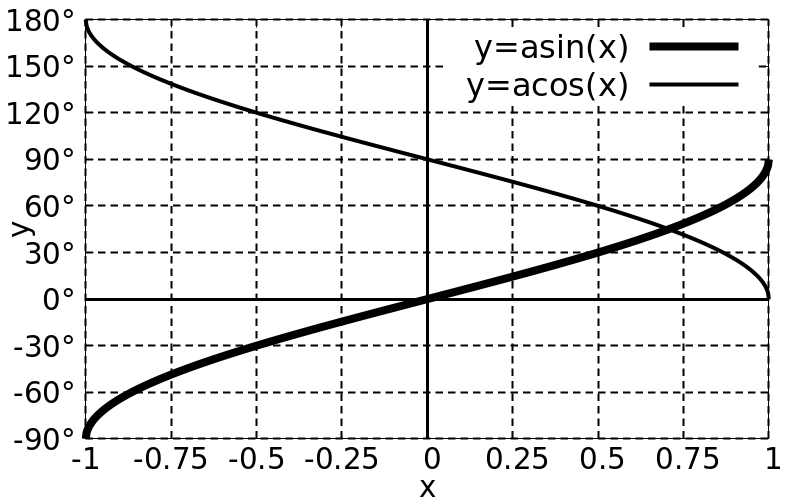
\includegraphics[width=7cm]{./gnuplot/base-function-arc}
        \caption{Graph zweier zyklometrischen Funktionen}
    \end{wrapfigure}
    \textbf{Zyklometrische Funktionen} (Arkusfunktion) sind die Umkehrung der trigonometrischen Funktionen. Der Definitionsbereich muss eingeschränkt werden, da die trigonometrischen Funktionen aufgrund ihrere Periodizität sonst nicht umkehrbar sind. Diese treten in der Praxis häufig auf, wenn Gleichungen mit trigonometrischen Funktionen zu lösen sind. Dabei ist unbedingt darauf zu achten, dass Lösungen nicht vergessen werden. Soll etwa $\sin(x)=1$ gelöst werden, liefert die naive Anwendung der Arkussinusfunktion $\text{asin}(1) = \degrees{90}$ und lässt die Lösungen $\dots, \degrees{-270}, \degrees{450}, \dots$ außen vor. Notiert werden sie als $\text{asin}$, $\text{acos}$ und $\text{atan}$, wobei das \emph{a} für \emph{arcus} oder \emph{Ark} (Bogen) steht. Die Funktionswerte sind Winkel, welche als Länge eines Kreisbogens mit diesem Winkel interpretiert werden können. Manchmal werden diese Funktionen auch als $\sin^{-1}$, $\cos^{-1}$ und $\tan^{-1}$ notiert. Dies ist immer im Sinne der Umkehrfunktion und nie als Reziprokenbildung zu verstehen.
\end{minipage}

\begin{minipage}[t]{1\textwidth}
    \begin{wrapfigure}{R}{7cm}
        \label{fig:ExBaseFunTan}
        \centering
        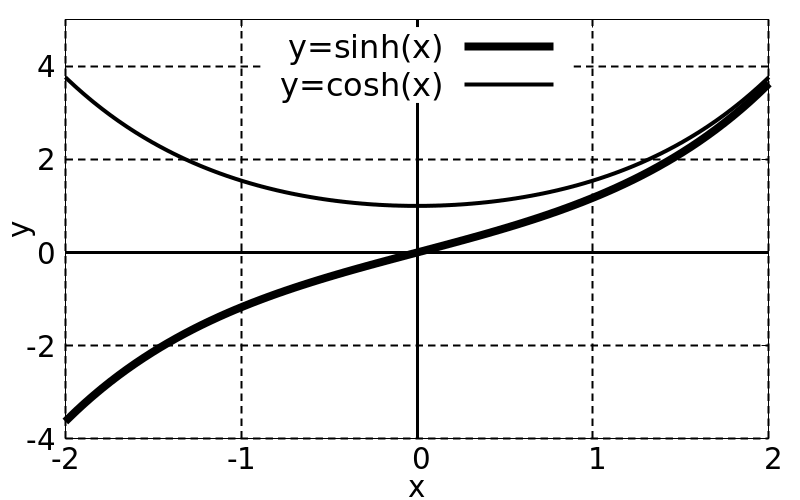
\includegraphics[width=7cm]{./gnuplot/base-function-hyp}
        \caption{Graph der hyperbolischen Funktionen}
    \end{wrapfigure}
    Die trigonometrischen Funktionen Sinus und Kosinus lassen sich mithilfe komplexer Zahlen und der Exponentialfunktion darstellen als $\cos(x) = \frac{e^{jx}+e^{-jx}}{2}$ und $j\cdot \sin(x) = \frac{e^{jx}-e^{-jx}}{2}$. Anders ausgedrückt können Sinus- und Kosinusfunktion also als gerader (achsensymmetrischer) und ungerader (punktsymmetrischer) Anteil der Exponentialfunktion für imaginäre Argumente betrachtet werden. Analog dazu werden die \textbf{hyberbolischen Funktionen} definiert als gerade und ungerader Anteil der Exponentialfunktion für reelle Argumente: $\text{cosh}(x) = \frac{e^x+e^{-x}}{2}$ (Hyperbelkosinus, \emph{cosinus hyperbolicus}) und $\text{sinh}(x) = \frac{e^x-e^{-x}}{2}$ (Hyperbelsinus, \emph{sinus hyberbolicus}).
\end{minipage}


\begin{figure}[h]
    \label{fig:LogScalePlot}
    \centering
    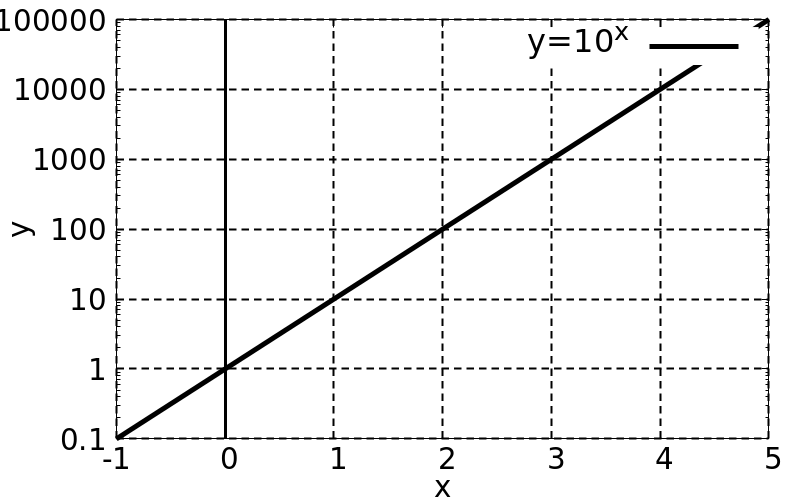
\includegraphics[width=0.6\textwidth]{./gnuplot/log-scale-plot}
    \caption{Graph von $10^x$ mit logarithmischer Einteilung der Ordinate}
\end{figure}

\clearpage

Polynome
Gebrochenrat. Fkt.

\section{Polynomdivision und Partialbruchzerlegung}

TOOD

% Definition, solving techniques, graphical interpretation
% 2D: Partial derivative and area/volume integral
\chapter{Infinitesimalrechnung}

Die Infinitesimalrechnung beschäftigt sich mit der Analyse stetiger Funktionen. In diesem Kapitel werden wir zuerst die Ableitung und das Integral für ein- und mehrstellige Funktionen definieren. Anschließend betrachten wir Rechenregeln kennen lernen, mit den sich eine Funktion in der Praxis einfacher ableiten und integrieren lässt. Abschließend schauen wir uns noch an, wie mithilfe der Ableitung lokale Extremwerte bestimmt werden können.

\section{Begriff der Ableitung}

Motivation für den Ableitungsbegriff war es, beschreiben zu können, in welcher Art und wie schnell sich Funktionswerte an verschiedenen Stellen des Definitionsbereich ändern. Ein Auto, welches mit konstanter Geschwindigkeit fährt,  wird durch eine Gerade im Weg-Zeit-Diagramm beschrieben. Die Geschwindigkeit kann man jetzt auffassen als die Änderungsrate des Wegs bezüglich der Zeit, also wie viele Kilometer das Auto pro Stunde zurücklegt. Jetzt betrachten wir aber ein Auto, welches nicht mehr mit konstanter Geschwindigkeit fährt, sondern aus dem Stand von $0$ auf $100 \ukmh$ beschleunigt. Wie können wir nun die Geschwindigkeit definieren und messen? Aus der Erfahrung ist klar (wenn man auf das Tachometer schaut), dass die Geschwindigkeit zu jedem Zeitpunkt eine andere ist. Wir benötigen also eine Definition für die Geschwindigkeit zu \emph{einem Zeitpunkt}. Zu sagen, die Momentangeschwindigkeit sei die \emph{momentane Änderungsrate} des Wegs lässt zu wünschen übrig, denn wie kann sich der Weg zu einem Zeitpunkt ändern? Wir können uns diesem Problem nähern, indem wir uns zuerst klar machen, wie man die Geschwindigkeit in der Praxis messen würde. Wir würden messen, wie weit sich das Auto innerhalb eines kleinen Zeitintervalls, etwa $1$ Sekunde, fortbewegt hat und dann den zurückgelegten Weg durch die Zeit teilen. Wir erhielten damit einen Schätzwert für die Momentangeschwindigkeit innerhalb gewissen Fehlergrenzen. Um die Momentangeschwindigkeit besser zu messen, könnten wir das Zeitintervall verkleinern. Diese Idee, erst mit einem endlichen Zeitintervall zu beginnen und dieses dann zu verkleinern, ist die Grundidee für die mathematische Definition der Ableitung. Mittels des Grenzwertbegriffs können wir das Zeitintervall bis auf $0$ verkleinern und erhalten so die Geschwindigkeit als Ableitung der Weg-Zeit-Funktion.

\subsection{Ableitung einstelliger Funktionen}

\begin{definition}{Differenzierbarkeit und Ableitung}{DiffFun}
    Eine Funktion $f: \R \to \R$ heißt an der Stelle $x_0\in\mathbb{D}$ \textbf{ableitbar} (differenzierbar), wenn der Differenzenquotient konvergiert:
    $$
        \alpha = \lim\limits_{\epsilon\to 0} \frac{f(x+\epsilon) - f(x)}{\epsilon}
    $$
    Dieser Grenzwert heißt dann \textbf{Ableitung der Funktion an der Stelle $x_0$} und man schreibt: $f'(x_0) = \alpha$.
    Falls eine Funktion auf ihrem gesamten Definitionsbereich differenzierbar ist, heißt sie \textbf{differenzierbare Funktion} und die durch
    $$
    f': x \mapsto \lim\limits_{\epsilon\to 0} \frac{f(x+\epsilon) - f(x)}{\epsilon}
    $$
    definiert Funktion die \textbf{Ableitung} von $f$ nach $x$. Man schreibt auch dann gelegentlich auch $\dd{f}{x}$.
\end{definition}

Analog dazu definiert man auch die zweite Ableitung einer Funktion als die Ableitung der Ableitungsfunktion, die dritte Ableitung wieder als deren Ableitung und so weiter. Man schreibt $f''$ oder $\ddn{2}{f}{x}$ für die zweite Ableitung, $f'''$ oder $\ddn{3}{f}{x}$ für die dritte Ableitung. Für die $n$-te Ableitungen schreibt man statt den Strichen auch $f^{(n)}$ (man beachte die Klammern!).

\textbf{Anmerkung}: In der Physik schreibt man manchmal auch $\dot{f}$ für die \textbf{Ableitung einer Funktion nach der Zeit}.

\begin{figure}
    \centering
    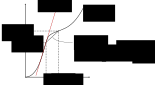
\includegraphics[width=0.8\textwidth]{./svg/derivative-function}
    \caption{Differenzenquotient einer Funktion}
    \label{fig:DiffFun}
\end{figure}

\begin{definition}{Lineare Näherung einer Funktion}{}
    Wenn eine Funktion $f$ an der Stelle $x_0$ differenzierbar ist, kann sie für kleine Abstände um diese Stelle herum durch eine Gerade $t$ genähert werden, welche man \textbf{Tangente} nennt und die gegeben ist durch:
    $$
        t: x \mapsto f(x_0) + f'(x_0) \cdot (x-x_0)
    $$
\end{definition}

Man kann sich auch vorstellen, man wählt sich eine Stelle $x_0$ und vergrößert den Graphen immer weiter um diese Stelle. Auch wenn die Funktion gesamt betrachtet gekrümmt sein mag, so wird sie, wenn sie denn differenzierbar ist, in der Vergrößerung aussehen wie eine Gerade. Diese Gerade nennt man dann Tangente.

\begin{example}{Bestimmung der Ableitung per Differenzenquotient}{DerivDiffQuot}
    Gesucht ist die Ableitung der Funktion $f(x) = x^2$ an einer Stelle $x_0$. Wir setzen in die Definition ein:
    \begin{alignat}{1}
        f'(x_0) &= \lim\limits_{\epsilon\to 0} \frac{f(x_0+\epsilon) - f(x_0)}{\epsilon} \\
                &= \lim\limits_{\epsilon\to 0} \frac{(x_0+\epsilon)^2-x_0^2}{\epsilon} \\
                &= \lim\limits_{\epsilon\to 0} \frac{x_0^2+2x_0\epsilon+\epsilon^2-x_0^2}{\epsilon} \\
                &= \lim\limits_{\epsilon\to 0} 2x_0+\epsilon \\
                &= 2x_0
    \end{alignat}
    Damit haben wir gezeigt, dass die quadratische Funktion überall differenzierbar ist und $f'(x) = \dd{}{x} x^2 = 2x$ gilt.
\end{example}

Eine wichtige Aussage über den Zusammenhang zwischen Stetigkeit und Differenzierbarkeit macht der folgende Satz:

\begin{statement}{Stetigkeit und Differenzierbarkeit}{ContDiffFun}
    Jede differenzierbare Funktion $f$ ist stetig. Die Stetigkeit ist also eine notwendige Bedingung für die Differenzierbarkeit, jedoch keine hinreichende Bedingung.
\end{statement}

\begin{example}{Stetige nicht differenzierbare Funktionen}{ContNonDiffFun}
    Die Betragsfunktion $f(x) = |x|$ ist für alle reellen Zahlen definiert und dort überall stetig. Speziell ist sie auch an der Stelle $x_0=0$ stetig. Allerdings ist sie dort nicht differenzierbar, denn
    der Grenzwert
    $$
        \lim\limits_{\epsilon\to 0} \frac{f(0+\epsilon) - f(0)}{\epsilon} = \lim\limits_{\epsilon\to 0} \frac{|\epsilon|}{\epsilon} = \lim\limits_{\epsilon\to 0} \text{sgn}(\epsilon)
    $$
    existiert nicht (siehe Beispiel \ref{ex:ExamContUnivarFun}). Graphisch betrachtet hat die Betragsfunktion bei $0$ einen Knick, der bestehen bleibt, egal, wie weit man den Knick vergrößert (sich also nicht als Gerade annähern lässt).
\end{example}

Es sei angemerkt, dass es auch Funktionen gibt, die überall stetig aber nirgends differenzierbar sind, ein Beispiel dazu findet sich im Anhang \ref{fig:BlancmangeFunction}.

Für viele Zusammenhänge ist es erforderlich, dass auch Ableitung selbst wieder eine stetige Funktion ist. Man definiert daher:

\begin{definition}{Stetige Differenzierbarkeit}{ContDiff}
    Eine Funktion $f$ heißt stetig differenzierbar, wenn sie differenzierbar ist und ihre Ableitung eine stetige Funktion ist.
\end{definition}

\begin{example}{Physikalische Anwendung der Ableitung}{}
    Eine Kreisbewegung in der $x$-$y$-Ebene mit konstanter Winkelgeschwindigkeit $\omega$ wird beschrieben durch $x(t) = r \cos(\omega t)$ und $y(t) = r \sin(\omega t)$, wobei $t$ die Zeit und $r$ den Radius des Kreises meint. Die erste Ableitung nach der Zeit lautet $v_x(t) = \dot{x}(t) = -r \omega \sin(\omega t)$, $v_y(t) = \dot{y}(t) = r \omega \cos(\omega t)$. Dabei handelt es sich um die x- und y-Komponenten der Geschwindigkeit $\vec v$, deren Betrag durch $|\vec v| = \sqrt{v_x^2+v_y^2} = r \omega$ gegeben ist. Damit haben wir die Formel für die Geschwindigkeit einer kreisförmigen Bewegung erhalten: $v = \omega r = 2\pi f r = \frac{2\pi r}{T}$ ($f\dots$Frequenz, $T\dots$ Periodendauer). Weiter können wir die zweite Ableitung bilden: $a_x(t) = \ddot{x}(t) = -r\omega^2 \sin(\omega t)$, $a_y(t) = \ddot{y}(t) = -r \omega^2 \sin(\omega t)$. Wir erhalten die x- und y-Komponenten der Beschleunigung $\vec a$, deren Betrag $|\vec a| = r \omega^2$ lautet. Das ist die Formel für die Beschleunigung bei einer Kreisbewegung: $a = \omega^2 r = \frac{v^2}{r}$. Die Zentripetalkraft (beziehungsweise Zentrifugalkraft in einem mitbewegten Inertialsystem) beträgt dann $F_Z = m \cdot a = m \frac{v^2}{r}$.
\end{example}

\subsection{Ableitung mehrstelliger Funktion}

Bisher haben wir die Ableitung nur für einstellige Funktionen betrachtet. Für mehrstellige Funktionen gibt es ein analoges Konzept, welches man die partielle Ableitung nennt. Der Funktionswert einer mehrstelligen Funktion wie etwa $f(x,y) = x^2+y^2$ hängt von mehreren Argumenten ab. Wir können aber alle Argumente bis auf eines festhalten (auf einen konstanten Wert setzen) und erhalten so wieder eine einstellige Funktion. Also beispielsweise $f(x,2) = x^2+4$. Diese einstellige Funktion entspricht einem Querschnitt durch den Graphen der zweistelligen Funktion, in diesem Fall dem Querschnitt durch die Ebene parallel zur $x$-$z$-Ebene. Ebenso hätten wir auch $x$ festhalten können und würden etwa $f(3, y) = y^2+9$ erhalten. Diese einstelligen Funktionen kann man nun ableiten und erhält die sogenannten partiellen Ableitungen, welche die Änderungsrate einer mehrstelligen Funktion in einer bestimmten Richtung beschreiben.

\begin{definition}{Partielle Ableitung}{PartDerivFun}
    Sei $f: \R^n\to\R$ eine mehrstellige Funktion. Die \textbf{partielle Ableitung} von $f$ nach $x_i$ ($1<i<n$) wird definiert als die Ableitung der einstelligen Funktion nach $x_i$, die entsteht, wenn man alle Argumente außer $x_i$ konstant hält. Man schreibt:
    \begin{alignat*}{1}
        \pdd{f}{x_i} \text { oder } f_{x_i} & \text{ für die erste Ableitung nach } x_i \\
        \pddn{2}{f}{x_i x_j} \text {oder } f_{x_i,x_j} & \text{ für die zweite Ableitung nach } x_i \text{ und } x_j
    \end{alignat*}
\end{definition}

Hierbei ist unbedingt auf die Reihenfolge der Ableitungen aufzupassen. $f_{xy}$ bezeichnet die Ableitung einer zweistelligen Funktion zuerst nach $x$ und dann nach $y$, $f_{yx}$ die Ableitung erst nach $y$ und anschließend nach $x$.

\begin{example}{Partielle Ableitungen}{PartDiff}
    \begin{itemize}
        \item Die partielle Ableitungen von $f(x,y) = x^2+y^2$ erhält man, indem man $x$ beziehungsweise $y$ als Konstante betrachtet und die Rechenregeln für das Differenzieren einstelliger Funktionen anwendet: $f_x = 2x$, $f_y = 2y$, $f_{xx} = 2$, $_{yy} = 2$.
        \item Die partielle Ableitung $f_z$ von $f(x,y) = \sin(x+\ln(y))$ lautet $f_z = 0$, da $z$ überhaupt nicht in $f$ vorkommt, die Funktionswerte sich somit bei Änderungen von $z$ nicht ändern.
    \end{itemize}
\end{example}

Im Beispiel \ref{ex:PartDiff} sehen wir, dass die beiden partiellen $f_{xy}$ und $f_{yx}$ übereinzustimmen scheinen, die Reihenfolge der Ableitungen also keine Rolle spielt. Es stellt sich daher die Frage, ob dies eine Ausnahme ist oder verallgemeinert werden kann. Der folgende Satz gibt darüber Auskunft:

\begin{statement}{Satz von Schwarz}{SchwarzTheo}
    Sei $f: \R^n \to \R$ ein mehrstelligen Funktion deren zweite partielle Ableitungen $f_{x_i x_j}$ und $f_{x_j x_i}$ stetig sind. Dann sind diese beiden Ableitungen gleich:
    $$
      f_{x_i x_j}, f_{x_j x_i} \text{ stetig}: \implies f_{x_i x_j} = f_{x_j x_i}
    $$
\end{statement}

$\pdd{f}{x}$ bezeichnet die partielle Ableitung eine bestimmten Funktion nach $x$. Um auszudrücken, dass man sich auf die Rechenoperation "\emph{Eine Funktion nach x ableiten}" bezieht, schreibt man $\pdd{}{x}$. Dieser Ausdruck ist ein sogenannten ¸\emph{Operator}, welcher auf beliebige Funktionen angewandt werden kann und eine neue Funktion zurückliefert, nämlich deren Ableitung nach $x$. Analog dazu ist $\dd{}{x}$ der \emph{Differentialoperator}, der einer einstelligen Funktion ihre Ableitung zuordnet.

Für mehrstellige Funktionen definiert man noch den sogenannten \mention{Nabla}-Operator, welcher sich zusammensetzt aus den einzelnen partiellen Ableitungen:

\begin{definition}{Nabla-Operator}{NablaOp}
    Für eine $n$-stellige Funktion bezeichnet $\vec \nabla = \rvec{\pdd{f}{x_1}}{\vdots}{\pdd{f}{x_n}}$ den Nabla-Operator. Dieser verhält sich wie ein Vektor und ordnet bei Anwendung auf eine Funktion ihr einen Vektor aus den partiellen Ableitungen zu.
\end{definition}

Dieser Operator ist nützlich, da er viele Formeln der Infinitesimalrechnung mehrstelliger Funktionen vereinfacht. Im letzten Kapitel haben wir bereits gesehen, dass man das Gradientenfeld einer mehrstelligen Funktion damit bündig schreiben kann als $\vec\nabla f$. Besonders bei Funktionen $\R^n \to \R^n$ wird der Nabla-Operator häufig verwendet. Da wir uns in dieser Vorlesung auf Funktionen $\R^n\to\R$ beschränken, werden wir den Nabla-Operator im Rahmen dieser Vorlesung kaum brauchen.

Schließlich können wir analog zur Tangenten für einstellige Funktionen noch eine sogenannten \emph{Tangentialebene} für zweistellige Funktionen definieren, also eine Ebene, die sich an die Funktion in einem Punkt anschmiegt. Diese Tangentialebene erhalten wir, wenn wir eine Ebene aufspannen, welche in $x$- und$y$-Richtung jeweils den Anstieg der Funktion in dieser Richtung hat. Dieser Anstieg ist durch die partiellen Ableitungen gegeben. Dieses Vorgehen lässt sich allgemein auf $n$-stellige Funktionen erweitern.

\begin{definition}{Lineare Näherung einer mehrstelligen Funktion}{LinApproxMultivarFun}
    Sei $f: \R^n\to\R$ ein $n$-stellige, partiell differenzierbare Funktion. Dann heißt $t$ die \textbf{lineare Näherung} der Funktion in einer kleinen Umgebung um einen Punkt $\vec{r_0}\in\R^n$ und ist gegeben durch:
    $$
        t(\vec r) = f(\vec{r_0}) +  \vec{\nabla}f(\vec{r_0}) \cdot (\vec{r} - \vec{r_0})
    $$
    Speziell für zweistellige Funktion $f(x,y)$ heißt $t$ die \textbf{Tangentialebene} und berechnet sich als:
    $$
        t(x,y) = t(x_0,y_0) + f_x(x_0,y_0) \cdot (x-x_0) + f_y(x_0,y_0) \cdot (y-y_0)
    $$
\end{definition}

Man beachte besonders, dass diese Formel für die lineare Näherung einer mehrstelligen Funktion identisch mit der Formel für die Tangentengleichung einer einstelligen Funktion ist, wenn man $n=1$ setzt.

\begin{example}{Bestimmung der linearen Näherung einer Funktion}{CompTangPlane}
    Gegeben sei die Funktion $f(x,y,z) =x^2+y^2+z$. Wir suchen die Gleichung der linearen Näherung an der Stelle $\vec{r_0} = (2,4,1)$. Um die Formel \ref{def:LinApproxMultivarFun} anwenden zu können, berechnen wir zuerst $\vec\nabla f$:
    $$
        \vec\nabla (x^2+y^2+z^2) = \rvec{\pdd{}{x} (x^2+y^2+z)}{\pdd{}{y} (x^2+y^2+z)}{\pdd{}{z} (x^2+y^2+z)} = \rvec{2x}{2y}{1}
    $$
    Dies setzen wir in die Formel ein und erhalten:
    \begin{alignat*}{1}
        t(x,y,z) &= t(x_0,y_0,z_0) + \rvec{2\cdot x_0}{2\cdot y_0}{z_0} \cdot \rvec{x-x_0}{y-y_0}{z-z_0} \\
                 &= t(2,4,1) + \rvec{2\cdot 2}{2\cdot 4}{1} \cdot \rvec{x-2}{y-4}{z-1} \\
                 &= 21 + 4 (x-2) + 8 (y-4) + (z-1)
    \end{alignat*}
\end{example}


\section{Begriff des Integrals}

\subsection{Einstellige Funktionen}

Die Ableitung können wir uns graphisch vorstellen als das Anlegen einer Tangente an eine Funktion. Ebenso könnten wir uns dem Integralbegriff über eine geometrische Fragestellung nähern. Wir betrachten zunächst einmal die Funktion $f(x) = \sin(x)$. Diese hat jeweils bei $0$ und bei $\pi$ eine Nullstelle. Wir stellen uns nun die Frage, wie groß der Flächeninhalt ist, den die Sinuskurve zwischen $0$ und $\pi$ mit der x-Achse einnimmt.

Um uns dieser Frage zu nähern, gehen wir auf ähnliche Weise zur Ableitung vor. Dort hatten wir zuerst Sekanten betrachtet und dann eine Grenzwertbildung vorgenommen, um die exakte Tangente zu erhalten. Genauso können wir für den Flächeninhalt mit einer Näherung anfangen, indem wir den Flächeninhalt unter der Sinuskurve durch kleine Rechtecke annähern, wie dies in Abbildung \ref{fig:ApproxAreaUnivarFun} dargestellt ist.

\begin{figure}
    \centering
    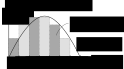
\includegraphics[width=0.6\textwidth]{./svg/integral-univariate-function}
    \caption{Annäherung des Flächeninhalts über Rechtecke}
    \label{fig:ApproxAreaUnivarFun}
\end{figure}

Wir zerlegen das Intervall $[a, b] = [0,\pi]$, für dem wir in den Flächeninhalt berechnen wollen, in die $n$ Teilintervalle $[x_i, x_{i+1}]$ ($0\le i \le n)$ mit der Länge $\Delta x_n = \frac{b-a}{n}$ . Dabei sind $x_i$ die Stützpunkte, welche sich ergeben zu $x_i = a + i\cdot\frac{b-a}{n} \cdot b$. Der Flächeninhalt $A_i$ ($1\le i \le n$) des $i$-ten Rechtecks berechnet sich als Breite mal Höhe. Die Breite ist gleich $\Delta x$, die Höhe entspricht dem Funktionswert $f(x_i)$ am $i$-ten Stützpunkt: $A_i = \Delta x \cdot f(x_i)$. Den gesamten Flächeninhalt $A$ erhalten wir, indem wir nun den Flächeninhalt aller Rechtecke aufaddieren:

\begin{alignat*}{1}
  A_n = \sum_{i=0}^{n-1} A_i &= \sum_{i=1}^{n} \frac{b-a}{n} f(a + i\cdot\frac{b-a}{n}) \\
                             &= \sum_{i=1}^{n} \Delta x_n f(a + i\cdot\Delta x) \\
\end{alignat*}

In Tabelle \ref{lst:ApproxIntegral} sind die Näherungswerte für einige $n$ angegeben.

\begin{listing}
    \begin{center}
        \begin{tabular}{ r | l}
            \textbf{Teilintervalle $n$} & \textbf{Näherungswert $A_n$} \\
            \hline
            1 & 0.00000 \\
            2 & 1.57079\dots \\
            3 & 1.81379\dots \\
            4 & 1.89611\dots \\
            5 & 1.93376\dots \\
            6 & 1.95409\dots \\
            7 & 1.96631\dots \\
            8 & 1.97423\dots \\
            9 & 1.97965\dots
        \end{tabular}
    \end{center}
    \caption[Näherungsweise Berechnung eines bestimmen Integrals]{Näherungswerte für den Flächeninhalt eingeschlossen durch den Graphen von $\sin(x)$ mit der x-Achse zwischen $0$ und $pi$.}
    \label{lst:ApproxIntegral}
\end{listing}

Wir sehen, je größer wir die Anzahl der Teilintervalle wählen, desto besser wird die Näherung (der genaue Wert lautet $2$). Mathematisch können wir dies fassen, in dem wir den Grenzwert für $n \to \infty$ bilden. Dies bringt uns zur Definition des bestimmten Integrals:

\begin{definition}{Bestimmtes Integral}{DefInteg}
    Das \textbf{bestimmte Integral} einer stetigen Funktion $f: \R \to \R$ im Intervall $[a,b] \subset \R$ ist der Grenzwert der Flächeninhaltssummen $A_n$, falls dieser existiert:
    $$
        \int\limits_{a}^b f(x) \diff{x} = \lim\limits_{n\to\infty} \sum_{i=1}^{n} \Delta x_n f(a + i\cdot\Delta x)
    $$
    Graphisch entspricht das bestimmte Integral dem \textbf{gerichteten Flächeninhalt} zwischen dem Graphen von $f$ unter der Abszisse (x-Achse). Der gerichtete Flächeninhalt ist positiv, wenn die Fläche oberhalb der Abszisse liegt, und negativ, wenn sie unterhalb der Abszisse liegt.
\end{definition}

\begin{example}{Berechnung des bestimmten Integrals}{CompDefInteg}
    \begin{itemize}
        \item Gesucht ist der Flächeninhalt zwischen $f(x) = x^2$ unter der x-Achse im Intervall $[0,1]$. Die Intervallänge lautet $\Delta x_n = \frac{b-a}{n} = \frac{1}{n}$. Die Funktionswerte an der Stützstelle $x_i = a + i \Delta x = \frac{i}{n}$ lauten $f(x_i) = \frac{i^2}{n^2}$. Eingesetzt in die Definition erhalten wir damit:
        \begin{alignat*}{1}
            A &= \lim\limits_{n\to\infty} \sum_{i=1}^{n} \Delta x_n f(a + i\cdot\Delta x) \\
              &= \lim\limits_{n\to\infty} \sum_{i=1}^{n} \frac{1}{n} \frac{i^2}{n^2} \\
              &= \lim\limits_{n\to\infty} \frac{1}{n^3} \sum_{i=1}^{n} i^2 \\
              &= \lim\limits_{n\to\infty} \frac{n^3/3+n^2/2+n/6}{n^3} \\
              &= \lim\limits_{n\to\infty} \frac{1}{3} + \frac{1}/{2n} + \frac{1}/{6n^2} \\
              &= \frac{1}{3}
        \end{alignat*}
        Wir haben dabei von der Formel zur Addition der Quadratzahlen Gebrauch gemacht: $1^2 + 2^2 + 3^2 + \dots + n^2 = \frac{n (n+1) (2n+1)}{6}$.
        \item Das bestimmte Integral über $\sin(x)$ zwischen $0$ und $2\pi$ lautet $0$, da der Flächeninhalt aus zwei betragsmäßig gleichen Teilen besteht, wobei der eine überhalb der x-Achse liegt und der andere Teil unterhalb der x-Achse. Der gerichtete Flächeninhalt des linken Teils ist somit positiv, der des rechten Teils, und in der Summe ergibt sich $0$.
    \end{itemize}
\end{example}

Nun ist es in der Praxis meist recht mühselig, jedesmal den Grenzwert ermitteln zu müssen. Glücklicherweise gibt es eine weitere Weise, das unbestimmte Integral zu berechnen. Dazu benötigen wir zuerst einmal die folgende Definition, welche man verstehen kann als Umkehroperation zum Differenzieren:

\begin{definition}{Stammfunktion und unbestimmtes Integral}{AntiDerivative}
    Eine Funktion $F$ heißt \textbf{Stammfunktion zu $f$}, wenn $f$ die Ableitung von $F$ ist: $\dd{F}{x} = f$. Die Menge aller Stammfunktionen nennt man das \textbf{bestimmte Integral} von $f$ und schreibt:
    $$
        \int f(x) \diff{x} = F(x) + C
    $$
    Dabei ist $C \in \R$ eine beliebige Konstante.
\end{definition}

Man beachte hierbei, dass es im Allgemeinen unbegrenzt viele Stammfunktionen gibt. Wenn $F$ eine Stammfunktion ist, kann man immer eine neue Funktion durch Addition mit einer konstanten Zahl bilden. Diese ist ebenfalls eine Stammfunktion, da das Addieren einer Konstant einem Verschieben der Funktion entlang der y-Achse entspricht und die Änderungsrate der Funktion nicht beeinflusst.

Der folgende Satz macht nun eine erstaunliche Aussage über den Zusammenhang zwischen dem bestimmten und dem unbestimmten Integral:

\begin{definition}{Hauptsatz der Differential- und Integralrechnung}{FundTheoCalc}
    Sei $F$ eine Stammfunktion von $f$, dann ist das bestimmte Integral im Intervall $[a,b]$  gleich der Differenz der Funktionswerte der Stammfunktion an den Intervallgrenzen:
    $$
        \int\limits_a^b = \left[F(x)\right]_a^b = F(b) - F(a)
    $$
\end{definition}

\begin{example}{Berechnung des bestimmten Integrals per Stammfunktion}{CompDefIntAntiDer}
    \begin{itemize}
        \item $F(x) = \frac{1}{3}x^3$ ist eine Stammfunktion von $f(x)=x^2$, wie man durch Ableiten von $F$ nachprüft. Der bestimmte Integral $\int\limits_0^1 x^2 \diff{x}$ ergibt sich somit zu $F(1)-F(0) = \frac{1}{3}$.
        \item Für $f(x) = \sin(x)$ ist $F(x) = -\cos(x)$ eine Stammfunktion. Somit ergibt sich für das bestimmte Integral $\int\limits_0^\pi \sin(x) = \left[-\cos(x)\right]_0^\pi = -\cos(\pi) - (-\cos(0)) = 2$.
    \end{itemize}
\end{example}

Eine wichtige Eigenschaft des bestimmten Integrals ist die Additivität der Grenzen. Wenn wir beispielsweise den (gerichteten) Flächeninhalt in den Intervallen $[0,1]$ und $[1,2]$ kennen, können wir daraus auch den (gerichteten) Flächeninhalt im Intervall $[0,2]$ ableiten, in dem wir die beiden einzelnen Flächeninhalt aufaddieren.

\begin{statement}{Additivität der Grenzen des bestimmten Integrals}{AddBoundDefInt}
    Das unbestimmte Integral einer Funktion $f$ über von $a$ bis $c$ lässt sich aufteilen in zwei unbestimmte Integrale mit einem Zwischenwert $b$:
    $$
    \int\limits_a^b f(x) \diff{x} + \int\limits_b^c f(x) \diff{x} = \int\limits_a^c f(x) \diff{x}
    $$
    Dies ist sogar dann gültig, wenn $b$ nicht zwischen $a$ und $c$ liegt.
\end{statement}

Der Beweis dazu folgt sofort aus dem Hauptsatz:

$$
    \int\limits_a^b f(x) \diff{x} + \int\limits_b^c f(x) \diff{x} = F(b) - F(a) + F(c) - F(b) = F(c) - F(a) = \int\limits_a^c f(x) \diff{x}
$$

\subsection{Mehrstellige Funktionen}


Nachdem wir uns nun angeschaut haben, wie man bestimmte Integrale eindimensionaler Funktionen berechnet, wollen wir den Begriff des bestimmten Integrals noch auf zweistellige Funktionen erweitern. Dies ist ein komplexes Themengebiet und daher hier nur auszugsweise dargestellt.

Um zu verstehen, was es bedeutet, eine zweistellige Funktion zu integrieren, erinnern wir uns nochmal, wie wir bei einstelligen Funktionen vorgegangen sind. Einstellige Funktionen haben eine Teilmenge der reellen Zahlen $\R^1$ als Definitionsbereich. Für die Definition des bestimmten Integrals haben wir diese eindimensionale Teilmenge (eine Gerade) in kleine Geradenstücke zerlegt. Für jedes Geradenstück haben wir dann dessen Länge $\Delta x$ multipliziert mit dem Funktionswert an dieser Stelle. Schließlich haben wir diese Werte alle aufaddiert.

Ersetzen wir nun "Gerade" durch "Fläche", "Geradenstück" durch "Flächenstück" und "Länge" durch "Flächeninhalt", erhalten wir die graphische Bedeutung des bestimmten Integrals einer zweistelligen Funktion $f(x,y)$ -- das Volumen, das der Graph der Funktion mit der x-y-Ebene einnimmt. Statt über ein eindimensionales Intervall zu integrieren, führen wir die Integration nun über eine Flächenstück der x-y-Ebene aus. Diese zerlegen wir in viele kleine Flächenstücke. Für jedes Flächenstück multiplizieren wir dessen Flächeninhalt mit dem Wert der Funktion an dieser Stelle und erhalten dadurch das Volumen des kleiner Quaders über diesem Rechteck. Abschließend addieren diese Werte auf.

Diese Vorgehensweise wollen wir uns noch anhand einer rechteckigen und eines kreisförmigen Fläche anschauen.

\subsection{Gebietsintegral in kartesischen Koordinaten}


Der Fall für eine rechteckige Fläche ist dargestellt in Abbildung \ref{fig:AreaIntegCartesian}.

\begin{figure}
    \centering
    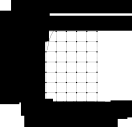
\includegraphics[width=0.48\textwidth]{./svg/integral-2d-cartesian}
    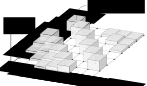
\includegraphics[width=0.48\textwidth]{./svg/integral-2d-cartesian-perspective}
    \caption[Gebietsintegral in kartesischen Koordinaten]{Graphische Interpretation eines Gebietsintegrals in kartesischen Koordinaten. Der Funktionswert an jedem kleinen schwarzen Punkt wird mit dem Flächeninhalt des Rechtecks multipliziert.}
    \label{fig:AreaIntegCartesian}
\end{figure}

Wir zerlegen nun analog zu einstelligen Funktionen das Rechteck $[a,b] \times [c,d]$, über das wir integrieren wollen, in $n\cdot m $ kleine Rechtecke $[x_i,x_{i+1}] \times [y_j,y_{j+1}]$. Jedes kleine Rechteck hat die Seitenlängen $\Delta x = \frac{b-a}{n}$ und $\Delta y = \frac{d-c}{m}$. Der Flächeninhalt des kleinen Rechtecks beträgt damit $A_{nm} = \Delta x \Delta y = \frac{(b-a)(c-d)}{nm}$. Die Stützpunkte lauten nun $x_i = a + i \Delta x$ und $y_j = c + j \Delta y$.  Nun multiplizieren wir den Flächeninhalt des Rechtecks mit dem Funktionswert und bilden die Summe. Wir erhalten:

\begin{center}
    \begin{alignat*}{1}
          & \lim\limits_{(n,m) \to (\infty, \infty)} \sum\limits_{j=1}^m \sum\limits_{i=1}^n f(x_i,y_j) \Delta x_n \Delta y_m  \\
        = & \int\limits_c^d \int\limits_a^b f(x,y) \diff{x} \diff{y}
    \end{alignat*}
\end{center}

Das letzte Gleichheitszeichen folgt aus der Definition des bestimmten Integrals für einstellige Funktionen. Wir sehen also, dass man ein mehrstelliges Integral durch Hintereinanderausführung normaler Integrale berechnen können. Statt über ein rechteckiges Gebiet zu integrieren, können wir auch über ein andersförmiges Gebiet integrieren, indem wir die Grenzen für die Integration über $x$ nicht auf einen festen Wert setzen, sondern von $y$ abhängen lassen (oder umgedreht). Wir erhalten damit das Gebietsintegral in kartesischen Koordinaten:

\begin{definition}{Gebietsintegral in kartesischen Koordinaten}{AreaIntCartCoord}
    Seien $u,v$ zwei einstellige Funktionen und $y_1,y_2\in\R$ zwei feste Zahlen. Dann wird durch $A = \left\lbrace (x,y) \in \R^2 | y \in [y_1,y_2] \land x \in [l(y), u(y)] \right\rbrace$ eine zweidimensionale Fläche beschrieben. Das Gebietsintegral einer Funktion $f$ über diese Fläche $A$ berechnet sich dann als:
    $$
        \int\limits_{A} f(x,y) \diff{A} = \int\limits_{y_1}^{y_2} \int\limits_{l(y)}^{u(y)} f(x,y) \diff{x} \diff{y}
    $$
\end{definition}

\begin{example}{Gebietsintegral in kartesischen Koordinaten}{AreaIntCarCoordTetra}
    Wir betrachten eine dreiseitige schiefe Pyramide, deren Spitze im Koordinatenursprung liegt und in Abbildung \ref{fig:AreaIntegTetraeder} dargestellt ist. Wir wollen das Volumen von diesem Körper berechnen. Der obere Punkte des Körpers in Abhängigkeit von $x$ und $y$ lautet $f(x,y) = 1-x-y$. $y$ bewegt sich dabei in den Grenzen $[0,1]$. Das Intervall für $x$ ist abhängig vom Wert von $y$. Die Untergrenze $l(y) = 0$ ist fest, die Obergrenze ist $u(y) = 1 - y$. Für das Volumen folgt nun unter über das Gebietsintegral:
    \begin{alignat*}{1}
        \int\limits_{A} f(x,y) \diff{A} & = \int\limits_{0}^{1} \int\limits_{0}^{1-y} (1-x-y) \diff{x} \diff{y} \\
                                        & = \int\limits_{0}^{1} \left[1-\frac{1}{2}x^2-y\right]_{0}^{1-y} \diff{y} \\
                                        & = \frac{1}{2} \int\limits_{0}^{1} y^2-2y+1 \diff{y} \\
                                        & = \frac{1}{2} \left[\frac{1}{3}y^3-y^2+y\right]_0^1 = \frac{1}{2} \cdot \frac{1}{3} = \frac{1}{6}
    \end{alignat*}
    Dies ist das erwartete Ergebnis für eine Pyramide mit der Grundfläche $A_G = \frac{1}{2}$ und der Höhe $h=1$: $V = \frac{1}{3} A_G h = \frac{1}{6}$.
\end{example}

\begin{figure}
    \centering
    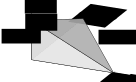
\includegraphics[width=0.65\textwidth]{./svg/integral-tetraeder}
    \caption{Gebietsintegrals für das Volumen einer schiefen Pyramide}
    \label{fig:AreaIntegTetraeder}
\end{figure}

\subsection{Gebietsintegral in Polarkoordinaten}

Abschließend wollen wir die gleiche Betrachtung noch einmal durchführen, aber mit dem Unterschied, dass die zu integrierende Fläche diesmal ein Kreis ist und wir sie nicht in kleine Rechtecke, sondern in kleine Kreissegmente zerlegen. Dies ist einfacher, als die Fläche in Rechtecke zu zerlegen. Bei der Zerlegung in Rechtecke würden im im Integral Wurzeln erscheinen, die sich meist nur schwer integrieren lassen.


In Abbildung \ref{fig:AreaIntegPolar} ist dieser Fall dargestellt. Wir gehen davon aus, dass der Kreis seinen Mittelpunkt im Koordinatenursprung besitzt und den Radius $R$ aufweist. Unsere Funktion hängt nun nicht mehr von $x$ und $y$ ab, sondern vom Abstand zum Ursprung $r$ und von Winkel mit der Abszisse $alpha$.

Das Vorgehen ist analog zum Vorgehen für Rechtecke. Wir zerlegen den Kreis mit $r\in[0,R]$ und $\alpha\in[0,,2\pi]$ in $n\cdot m$ kleine Kreissegmente mit Radius $[r_i, r_{i+1}]$ einem Winkel $[\alpha_j, \alpha_{j+1}]$. Jedes kleine Kreissegment kann näherungsweise als Rechteck aufgefasst werden mit den Seitenlängen $\Delta a = \Delta r_n$ und $\Delta b = r \Delta \alpha_n$ (siehe Skizze). Der Flächeninhalt des Kreissemgents ist daher etwa $A_{nm} = r \Delta r \Delta \alpha$. Die Stützpunkte lauten $r_i = 0 + i \Delta r_n$ und $y_j = j \Delta \alpha_m$. Wir multiplizieren den Flächeninhalt des Kreissegment mit dem Funktionswert und bilden die Summe. Es ergibt sich:

\begin{center}
    \begin{alignat*}{1}
      & \lim\limits_{(n,m) \to (\infty, \infty)} \sum\limits_{j=1}^m \sum\limits_{i=1}^n f(r_i,\alpha_j) r \Delta r_n \Delta \alpha_m  \\
    = & \int\limits_0^d \int\limits_0^\alpha f(r, \alpha) \diff{r} \diff{\alpha}
    \end{alignat*}
\end{center}

Analog kann man das Gebietsintegral auch für andere Flächen und Koordinatensystem angeben. Aus diesem Ergebnis können wir noch eine wichtige Erkenntnis ziehen. Während bei kartesischen Koordinaten nur über $x$ und $y$ integriert wurden, müssen wir in Polarkoordinaten noch einen zusätzlichen Faktor $r$ in das Integral einfügen. Je nach Koordinatensystem ist dies ein anderer Faktor, und nur im Spezialfall der kartesischen Koordinaten ist der Faktor $1$.

Wir können nun auch wieder statt festen Grenzen für $r$ diese von $\alpha$ abhängig machen. Der Vollständigkeit halber sei noch das Gebietsintegral in Polarkoordinaten analog zu den kartesischen Koordinaten definiert.

\begin{definition}{Gebietsintegral in Polarkoordinaten}{AreaIntPolar}
    Seien $u,v$ zwei einstellige Funktionen und $\alpha_1,\alpha_2\in\R$ zwei feste Zahlen. Dann wird durch $A = \left\lbrace (r,\alpha) \in \R^2 | \alpha \in [\alpha_1,\alpha_2] \land r \in [l(\alpha), u(\alpha)] \right\rbrace$ eine zweidimensionale Fläche beschrieben. Das Gebietsintegral einer Funktion $f$ über diese Fläche $A$ berechnet sich dann als:
    $$
    \int\limits_{A} f(r,\alpha) \diff{A} = \int\limits_{\alpha_1}^{\alpha_2} \int\limits_{l(\alpha)}^{u(\alpha)} f(r,\alpha) \cdot r \diff{r} \diff{\alpha}
    $$
\end{definition}

\begin{figure}
    \centering
    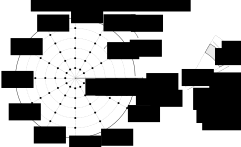
\includegraphics[width=0.95\textwidth]{./svg/integral-2d-polar}
    \caption[Gebietsintegral in Polarkoordinaten]{Graphische Interpretation eines Gebietsintegrals in Polarkoordinaten. Der Funktionswert an jedem kleinen schwarzen Punkt wird mit dem Flächeninhalt des Kreissegments multipliziert.}
    \label{fig:AreaIntegPolar}
\end{figure}

\begin{example}{Flächeninhalt des Kreises}{AreaIntPolarCircArea}
    Mithilfe des Gebietsintegral können wir auch den Flächeninhalt eines Kreises mit Radius $R$ berechnen, indem wir $f(r,\alpha) = 1$ setzen und über die Kreisfläche $r=0\dots R$ und $\alpha = 0\dots 2\pi$ integrieren:
    \begin{alignat*}{1}
        \int\limits_{A} f(x,y) \diff{A} &= \int\limits_0^{2\pi} \int\limits_0^R 1 r \diff{r} \diff{\alpha}  \\
                                        &= \int\limits_0^{2\pi} \frac{R^2}{2} \diff{\alpha} \\
                                        &= 2\pi \cdot \frac{R^2}{2} \\
                                        &= \pi R^2
    \end{alignat*}
    Damit haben wir nachgewiesen, dass der Flächeninhalt des Kreises sich tatsächlich zu $A =\pi R^2$ berechnet.
\end{example}

\section{Rechenregeln zum Differenzieren}

Um nun auch praktisch Ableitungen berechnen zu können, benötigen wir Zweierlei. Zum Einen müssen wir wissen, wie die Ableitung von Grundfunktionen (Potenz, Expoentialfunktion, Logarithmen, $\dots$) lautet. Diese kennt man entweder auswendig oder schlägt diese in Tafelwerken nach. Zum Zweiten benötigen wir noch Rechenregeln, mit denen wir aus Grundfunktionen zusammengesetzte Funktionen ableiten können. Diese sind in diesem Abschnitt kurz für einstellige Funktionen zusammengefasst.

\begin{statement}{Linearität des Differenzialoperators}{DiffOpLin}
    Der Differenzialoperator $\dd{}{x}$ ist \textbf{linear}. Sind $f$, $g$ zwei differenzierbare Funktionen und $\alpha,\beta\in\R$ zwei Konstanten, dann gilt:
    $$
        (\alpha f + \beta g)' = \alpha f' + \beta g'
    $$
\end{statement}

\begin{example}{Ableiten einer Linearkombination von Funktionen}{DiffLinCombFun}
    Die Ableitung des Polynoms $f(x) = 3x^2+6x$ ergibt sich, indem man die Monome $x^2$ und $x$ ableitet und entsprechend wieder zusammensetzt: $f'(x) = 3 * \dd{}{x} (x^2) + 6 \dd{}{x} x = 6x +6$.
\end{example}

Um ein Produkt oder Quotienten zweier Funktionen $h(x) = f(x) \cdot g(x)$ abzuleiten, betrachten wir den Grenzwert des Differenzenquotienten für $h$:

\begin{alignat*}{1}
    \dd{h}{x} &= \lim\limits_{\epsilon\to 0} \frac{h(x+\epsilon)-h(x)}{\epsilon} \\
              &= \lim\limits_{\epsilon \to 0} \frac{f(x+\epsilon)g(x+\epsilon)-f(x)g(x)}{\epsilon} \\
               &= \lim\limits_{\epsilon \to 0} \frac{f(x+\epsilon)g(x+\epsilon) \overbrace{-f(x)g(x+\epsilon) + f(x)g(x+\epsilon)}^{=0} - f(x)g(x)}{\epsilon} \\
               &= \lim\limits_{\epsilon \to 0} \frac{[f(x+\epsilon)-f(x)]\cdot g(x+\epsilon) + f(x) \cdot [g(x+\epsilon) - g(x)]}{\epsilon} \\
               &= \underbrace{\lim\limits_{\epsilon \to 0} \frac{f(x+\epsilon)-f(x)}{\epsilon}}_{=f'(x)} \underbrace{\lim\limits_{\epsilon\to 0} g(x+\epsilon)}_{=g(x)\text{, da g stetig}} + f(x) \underbrace{\lim\limits_{\epsilon \to 0} \frac{g(x+\epsilon)-g(x)}{\epsilon}}_{=g'(x)} \\
               &= f'(x)g(x) + f(x) g'(x)
\end{alignat*}

Damit haben wir die sogenannte Produktregel erhalten:

\begin{statement}{Produktregel}{ProdRule}
    Sind $f$ und $g$ zwei differenzierbare Funktionen, dann berechnet sich die Ableitung des Produkts der beiden Funktionen mittels der \textbf{Produktregel}:
    $$
        (f \cdot g)' = f' \cdot g + f \cdot g'
    $$
\end{statement}

\begin{example}{Ableiten eines Produkts zweier Funktionen}{CompDiffProdFun}
    Die Ableitung der Funktion $f(x) = x^2 \sin(x)$ berechnet sich mittels der Produktregel zu $f'(x) = \dd{}{x} (x^2) \cdot  \sin(x) + x^2 \dd{}{x} \sin(x) = 2x\sin(x) + x^2\cos(x)$.
\end{example}

Um eine Komposition (Verknüpfung) zweier Funktionen abzuleiten, hilft die Kettenregel, welche wir hier ohne Herleitung angeben:

\begin{statement}{Kettenregel}{ChainRule}
    Sind $f$ und $g$ zwei differenzierbare Funktionen, dann berechnet sich die Ableitung der Komposition der beiden Funktionen mittels der \textbf{Kettenregel}:
    $$
        (f \circ g)' = f' \cdot g'
    $$
    Dabei heißt $f'$ äußere Ableitung und $g'$ innere Ableitung.
\end{statement}

\begin{example}{Ableiten einer verknüpften Funktion}{CompDiffChainFun}
    \begin{itemize}
        \item Um $h(x) = (3x^2+5)^4$ abzuleiten, setzen wir $f(g) = g^4$ und $g(x) = 3x^2+5$. Deren Ableitungen sind $f'(g) = 4g^3$ (äußere Ableitung) und $g'(x) = 6x$ (innere Ableitung). Wir erhalten: $h'(x) = 4g^3 \cdot 6x = 24x(3x^2+5)^3$
        \item Die Ableitung der Funktion $h(x) = \sin(x^2)$ berechnet sich mit der äußeren Ableitung $\cos(g)$ und der inneren Ableitung $2x$ zu $h'(x) = 2x\cos(x^2)$.
    \end{itemize}
\end{example}

\begin{example}{Ableiten des Hyperbelsinus und Hyperbelkosinus}{CompDerSinh}
    Der Hyperbelsinus ist definiert als $\frac{1}{2} (e^x - e^{-x})$, der Hyperbelkosinus als $\frac{1}{2} (e^x + e^{-x})$. Mithilfe der Kettenregel finden wir $\dd{}{x}e^{-x} = -e^{-x}$ und erhalten damit für die Ableitung des Hyperbelsinus:
    $$
        \dd{}{x} \text{sinh}(x) = \frac{1}{2} (e^x-(-e^{-x})) = \text{cosh(x)}
    $$
    Analog erhält man für den Hyperbelkosinus:
    $$
        \dd{}{x} \text{cosh}(x) = \frac{1}{2} (e^x+(-e^{-x})) = \text{sinh(x)}
    $$
    Im Gegensatz zu den trigonometrische Funktionen, wo bei der Ableitung des Kosinus auf das Minuszeichen zu achten ist ($\sin(x)' = \cos(x)$, $\cos(x)' = -\sin(x)$), sind die hyperbolischen Funktionen in dieser Hinsicht symmetrisch: $\text{sinh}(x)' = \text{cosh}(x)$, $\text{cosh}(x)' = \text{sinh}(x)$.
\end{example}

\begin{example}{Ableiten eines Quotienten zweier Funktionen}{CompDiffQuotFun}
    Sei $h(x) = f(x) / g(x)$ ein Quotient zweier Funktionen. Um diesen Abzuleiten, schreiben wir $h$ als Produkt $f(x) \cdot \frac{1}{g(x)}$ und wenden die Produktregel in Kombination mit der Kettenregel an:
    \begin{alignat*}{1}
        h' &= f' \cdot \frac{1}{g} + f \cdot \left(-\frac{1}{g^2} \cdot g'\right) \\
           &= \frac{f'g - fg'}{g^2}
    \end{alignat*}
    Dies wird gelegentlich auch als \emph{Quotientenregel} bezeichnet.
\end{example}

\begin{example}{Ableitung des Tangens}{CompDiffTan}
    Die Ableitung des Tangens $\tan(x) = \frac{\sin(x)}{cos(x)}$ berechnet sich mithilfe der Quotientenregel zu:
    \begin{alignat*}{1}
        \dd{}{x} \tan(x) &= \frac{\cos(x)\cos(x)-(-\sin(x)\sin(x))}{\cos^2(x)} \\
                         &= \frac{\sin^2(x) + \cos^2(x)}{\cos^2(x)} \\
                         &= \frac{1}{\cos^2(x)} \\
                         &= 1+\frac{\sin^2(x)}{\cos^2(x)} = 1 + \tan^2(x)
    \end{alignat*}
\end{example}

Wenn eine Funktion $f(x)$ eine Umkehrfunktion $g(y) = f^{-1}(y)$ besitzt, können wir mithilfe der Kettenregel eine Formel für die Ableitung der Umkehrfunkion herleiten. Es gilt $g(f(x)) = x$, da $g$ die Umkehrfunktion zu $f$ ist. Es folgt:

\begin{alignat*}{1}
    g(f(x)) &= x \\
    \dd{}{x} g(f(x)) &= \dd{}{x} x \\
    g'(f(x)) \cdot f'(x) &= 1 \\
    g'(y) \cdot f'(x) &= 1
\end{alignat*}

Dies ist im folgenden Satz zusammengefasst:

\begin{statement}{Ableitung der Umkehrfunktion}{InverseFunDiffRule}
    Sei $f$ eine differenzierbare Funktion mit der Umkehrfunktion $f^{-1}$. Zwischen der Ableitung von $f$ und ihrer Umkehrfunktion gilt dann folgende Beziehung:
    $$
        f' \cdot (f^{-1})' = 1
    $$
\end{statement}

\begin{example}{Ableitung des Arkustangens}{CompDiffArctan}
    Die Ableitung der Arkustangensfunktion können wir mithilfe der Regel zur Ableitung von Umkehrfunktionen berechnen. Wir setzen $y = f(x) = \tan(x)$. Dann gilt:
    \begin{alignat*}{1}
        \dd{}{y} \arctan(y) &= \frac{1}{\dd{}{x} \tan(x)} \\
                            &= \frac{1}{\underbrace{\tan^2(x)}_{=y^2}} \\
                            &= \frac{1}{1+y^2}
    \end{alignat*}
\end{example}

\begin{example}{Ableitung des Arkussinus}{CompDiffArcsin}
    Die Ableitung der Arkussinusfunktion können wir ebenfalls mit der Regel zur Ableitung von Umkehrfunktionen berechnen. Wir erhalten:
    \begin{alignat*}{1}
        & \dd{}{x} \sin(x) \dd{}{y} \text{asin}(y) = 1 \\
        & \dd{}{y} \text{asin}(y) = \frac{1}{\cos(x)} = \frac{1}{\cos(\text{asin}(y))}
    \end{alignat*}
    Diesen Ausdruck können wir noch vereinfachen. Nach dem Satz des Pythagoras gilt $\sin^2(x) + \cos^2(x) = 1$ und damit können wir umformen:
    \begin{alignat*}{1}
        \cos(\text{asin}(x)) &= \sqrt{1 -  \sin^2(\text{asin}(x))} \\
                             & = \sqrt{1 - x^2}
    \end{alignat*}
    Also gilt für die Ableitung des Arkussinus:
    $$
        \dd{}{x} \text{asin}(x) = \frac{1}{\sqrt{1-x^2}}
    $$
\end{example}

\begin{example}{Ableitung des Arkuskosinus}{CompDiffArccos}
    Für die Ableitung der Arkuskosinusfunktion erhalten wir analog $\dd{}{y} \text{acos}(y) = -\frac{1}{\sin(\text{acos}(x))}$. Mittels $\sin(\text{acos}(x)) = \sqrt{1 - \cos^2(\text{acos}(x))}$ wird daraus:
    $$
        \dd{}{x} \text{acos}(x) = -\frac{1}{\sqrt{1-x^2}}
    $$
\end{example}


\section{Rechenregeln zum Integrieren}

Um nun auch praktisch Stammfunktionen berechnen zu können, benötigen wir Zweierlei. Zum Einen müssen wir wissen, wie die Stammfunktion von Grundfunktionen lautet. Diese kennt man entweder auswendig oder schlägt diese in Tafelwerken nach. Auf eine Stammfunktion sei aber noch einmal explizit hingewiesen, da es bei dieser oft ein Teil vergessen wird:

\begin{statement}{Stammfunktion der Hyperbel}{AntiDerHyp}
    Die Menge aller Stammfunktionen von $f(x) = \frac{1}{x}$ ist gegeben durch $F(x) = \ln(|x|) + C$
\end{statement}

Nicht vergessen werden darf der Betrag im Logarithmus -- denn $1/x$ ist sowohl für positive als auch für negative Werte definiert, $\ln(x)$ aber nur für positive Werte. Eine Weitere Stammfunktion, die manchmal hilfreich ist, lautet:

\begin{statement}{Stammfunktion der Betragsfunktion}{AntiDerSignum}
    Die Menge aller Stammfunktionen der Betragsfunktion $f(x) = \text{sgn}(x)$ ist gegeben durch $F(x) = |x| = \sqrt{x^2} + C$
\end{statement}

Zum Zweiten benötigen wir noch Rechenregeln, mit denen wir auch Stammfunktionen für aus Grundfunktionen zusammengesetzte Funktionen bilden können. Diese sind in diesem Abschnitt kurz für einstellige Funktionen zusammengefasst.

\textbf{Bei der Bildung des unbestimmten Integrals ist unbedingt auf die Integrationskonstante zu achten.} Später im Kapitel zu Differentialgleichungen werden wir feststellen, dass diese Integrationskonstante wichtig ist, da sonst viele Lösungen einer Differentialgleichung "übersehen" werden.

\begin{statement}{Linearität des Integraloperators}{IntOpLin}
    Der Integraloperator $\int \diff{x}$ ist \textbf{linear}. Sind $f$, $g$ zwei integrierbare Funktionen und $\alpha,\beta\in\R$ zwei Konstanten, dann gilt:
    $$
    \int (\alpha f + \beta g) \diff{x} = \alpha \int f \diff{x} + \beta \int g \diff{x}
    $$
\end{statement}

\begin{example}{Stammfunktion einer Linearkombination von Funktionen}{LinComAntiDer}
    Das unbestimmte Integral des Polynoms $f(x) = 3x^2+6x$ ergibt sich, indem man die Monome $x^2$ und $x$ integriert und entsprechend wieder zusammensetzt: $\int f(x) \diff{x} = 3 \int x^2 \diff{x} + 6 \int x \diff{x} = x^3 + 3 x^2 + C$.
\end{example}

Um ein Produkt zweier Funktionen zu integrieren, formen wir die Produktregel geschickt um. Wir betrachten zwei Funktion $f$ und $g$, wobei $F$ eine Stammfunktion von $f$ bezeichnet. Nach der Produktregel gilt dann:

\begin{alignat*}{1}
    (Fg)' &= F'g + Fg' \\
          &= fg + Fg'
\end{alignat*}

Beiden Seiten der Gleichung können wir nach $x$ integrieren und erhalten:

$$
  Fg = \int fg \diff{x} + \int Fg' \diff{x}
$$

Bringt man jetzt noch den rechten Summanden auf die linke Seite, erhält man die sogenannte Regel für die \emph{partielle Integration}:

\begin{definition}{Partielle Integration}{IntByParts}
    Seien $f,g$ zwei integrierbare Funktionen und $F$ eine Stammfunktion von $f$. Dann gilt für das unbestimmte Integral des Produkts beider Funktionen:
    $$
      \int f(x) \cdot g(x) \diff{x} = F(x) \cdot g(x) - \int F(x) g'(x) \diff{x}
    $$
\end{definition}

Im Gegensatz zur Produktregel gibt es einen bedeutsamen Unterschied. Die Produktregel reduziert das Problem, ein Produkt zweier Funktionen abzuleiten darauf, die beiden Einzelfunktionen abzuleiten. Das gleiche gilt für andere Ableitungsregeln. Durch sukzessive Anwendung der Ableitungsregeln kann daher die Ableitung einer zusammengesetzten Funktion immer auf die Ableitung der Grundfunktionen reduziert werden. Dies ist bei der partiellen Integration nicht der Fall. Um die Regeln erfolgreich anwenden zu können, müssen wir das Integral auf der rechten Seite bestimmen können. Im Integranden steht nun aber das Produkt der Stammfunktion und der Ableitung der anderen Funktionen. Im Allgemeinen gibt es keine Garantie dafür, dass dieses Integral einfacher zu bestimmen ist als das ursprüngliche Integral. Tatsächlich ist es so, dass selbst einfache Kombinationen von Grundfunktionen nicht mehr elementar integrierbar sind. Beispielsweise ist es nicht möglich, $\int \frac{\sin(x)}{x} \diff{x}$ nur mittels Grundfunktionen zu schreiben.

Bei der Anwendung der Produktregel sollte man daher vorher immer nachdenken, ob das auf der rechten Seite entstehende Integral lösbar sein wird. Da es sich um Produkt zweier Funktionen handelt, hat man zudem zwei Möglichkeiten für die Wahl, welche Funktion man ableitet und von welcher man die Stammfunktion bildet. Oft führt nur eine Wahl zum Ziel.

\begin{example}{Stammfunktion eines Produkts}{CompAntiDerProd}
    Gesucht ist das unbestimmte Integral von $f(x) = x e^x$. Dies wollen wir mittels partieller Integration finden. Die Funktion ist ein Produkt aus $x$ und $e^x$. Zuerst müssen wir überlegen, von welchem Faktor wir die Ableitung und von welchem Faktor wir die Stammfunktion bilden wollen. Wenn wir von $x$ eine Stammfunktion nehmen würden und von $e^x$ die Ableitung, müssten wir dann auf der rechten Seite ein Integral der Form $x^2 e^x$ lösen -- dies wird nicht einfacher sein. Wählen wir stattdessen $x$ zum Ableiten aus, wird die rechte Seite einfacher werden, da die Ableitung dann $1$ ist. Wir erhalten:
    $$
        \int x e^x \diff{x} = x e^x - \int 1 \cdot e^x \diff{x} = xe^x-e^x + C = (x-1) e^x + C
    $$
\end{example}

\begin{example}{Stammfunktion des Logarithmus}{CompAntiDerLog}
    Mittels partieller Integration kann auch der Logarithmus $f(x) = \ln(x)$ integriert werden. Dazu schreiben wir $f(x) = 1 \cdot \ln(x)$ und erhalten:
    $$
        \int 1\cdot\ln(x) = x\ln(x) - \int x/x \diff{x} = x\ln(x)-x+C = x (\ln(x) - 1) + C
    $$
\end{example}

\begin{example}{Stammfunktion des Produkts von Sinus und Kosinus}{CompAntiDerSinCos}
    Manchmal muss man nach Anwendung der partiellen Integration noch geschickt umstellen, um zum Ziel zu kommen. Für $f(x) \sin x\cos x$ erhält man beispielsweise:
    $$
        \int \sin x \cos x \diff{x} = \sin^2 x - \int \sin x \cos x \diff{x}
    $$
    Auf beiden Seiten der Gleichung kommt nun das zu bestimmende unbestimmte Integral vor. Wir können die Gleichung danach umstellen und erhalten:
    $$
        \int \sin x \cos x \diff{x} = \frac{1}{2} \sin^2 x + C
    $$
\end{example}

Analog zur Kettenregel zum Ableiten gibt es auch eine Entsprechung für das unbestimmte Integral. Um diese herzuleiten, betrachten wir zwei Funktion $f$ und $u$ und bezeichnen mit $F$ eine Stammfunktion von $f$. Für die Komposition $F \circ u$ beider Funktionen gilt nun einerseits:

$$
    (F\circ u)' = F' \cdot u' = f \cdot u'
$$

Wobei $(\dots)'$ die Ableitung nach $x$ bezeichnet. Es folgt

\begin{equation}
    \int (F \circ u)' \diff{x} = \int f \cdot u' \diff{x} \label{eq:IntPartsProof1}
\end{equation}

Andererseits gilt aber auch:

\begin{equation}
    \int (F \circ u)' \diff{x} = F \circ u = F(u) = \int f(u) \diff{u} \label{eq:IntPartsProof2}
\end{equation}

Durch Gleichsetzen von \ref{eq:IntPartsProof1} und \ref{eq:IntPartsProof1} erhalten wir die sogenannte Integration durch Substitution:

\begin{statement}{Integration durch Substitution}{IntSubst}
    Sei $f$ eine integrierbare Funktion und $u$ eine sogenannte Substitutionsfunktion. Dann gilt:
    $$
        \int f(u) \diff{u} = \int f(u(t)) u'(t) \diff{t}
    $$
\end{statement}

Bei Anwendung der obigen Regel müssen wir beachten, dass wir bei einem der beiden unbestimmten Integrale die Integrationskonstante nicht vergessen. Für die tatsächliche Berechnung ist meist das folgende Vorgehen praktikabler. Dazu müssen wir uns noch einmal daran erinnern, dass die Ableitung über den Anstieg einer Tangente definiert war. Die Tangente ist eine Gerade und der Anstieg von Gerade ist gegeben als der Quotient $\frac{\Delta y}{\Delta x}$ der Änderung des Funktionswerts und der Änderung des Arguments. Die symbolische Schreibweise $\dd{y}{x}$ können wir auch auffassen als Quotient zweier \emph{infinitesimalen} Größen $\diff{y}$ und $\diff{x}$. Diese Schreibweise nennt man \textbf{Leibniz-Notation}. Wenn wir $\dd{y}{x}$ als Bruch betrachten und damit rechnen, als wäre es ein Bruch, sind einige Formeln manchmal einfacher verständlich. Die Regel zur Ableitung der Umkehrfunktion (siehe \ref{stmt:InverseFunDiffRule}) lautet in dieser Schreibweise etwa $\dd{y}{x} \dd{x}{y} = 1$, was nach den Regeln der Bruchrechnung offensichtlich korrekt ist. Wir erhalten dann das folgende alternative Verfahren für die Integration durch Substitution:

\begin{enumerate}
    \item Wähle aufgrund der Form der zu integrierenden Funktion $f$ eine Substitution $u(x)$.
    \item Berechne die Ableitung $u'(x) = \dd{u}{x}$
    \item Forme um nach $\diff{}{x} = \frac{\diff{u}}{u'}$
    \item Ersetze nun in $\int f(x) \diff{x}$ das Argument durch $u$ und $\diff{x}$ durch $\frac{\diff{u}}{u'}$
    \item Berechne das entstehende Integral nach $u$ und ersetze abschließend wieder $u$ durch $x$.
\end{enumerate}

\begin{example}{Anwendung der Integration durch Substitution}{CompAntiDerSubst}
    Gesucht ist das Integral $\int x \cos(x^2) \diff{x}$. Dies können wir so nicht berechnen, da wir nicht wissen, wie wir einen Kosinus mit $x^2$ im Argument integrieren sollen. Es wäre schon, wenn im Argument nur $x$ stehen würde. Um das zu erreichen, wählen wir für die Substitution $u = x^2$. Die Ableitung lautet $\dd{u}{x} = 2x$. Das stellen wir um zu $\diff{x} = \frac{\diff{u}}{2x}$. Nun können wir im ursprünglichen Integral substituieren:
    \begin{alignat*}{1}
        \int x \cos(x^2) \diff{x} &= \int x \cos(u) \frac{\diff{u}}{2x} \\
                                  &= \frac{1}{2} \int \cos(u) \diff{u} \\
                                  &= \frac{1}{2} \sin(u) + C \\
                                  &= \frac{1}{2} \sin(x^2) + C
    \end{alignat*}
\end{example}

Wie bereits im vorigen Kapitel erwähnt, können gebrochenrationale Funktionen mittels Polynomdivision und Partialbruchzerlegung integriert werden. Die Polynomdivision formt eine unecht gebrochenrationale Funktion um in die Summe aus einem Polynom (was einfach zu integrieren ist) und einer echt gebrochenrationalen Funktion. Letztere kann mittels Partialbruchzerlegung in eine Summe aus Partialbrüchen zerlegt werden, die einfacher integrierbar sind. Beispielsweise haben wir im letzten Kapitel gesehen, dass sich $\frac{x}{x^2-1}$ zerlegen lässt in die beiden Partialbrüche $\frac{1/2}{x-1} + \frac{1/2}{x+1}$. Diese sind unmittelbar integrierbar: $\frac{1}{2}\ln(|x-1|) + \frac{1}{2} \ln(|x+1|) + C$.

\section{Extremwertbestimmung}

Ein Anwendungsfall der Differentialrechnung ist das Bestimmen von lokalen Extremwerten. Ein lokaler Extremwert ist gerade dadurch charakterisiert, dass die Funktion sich dort kaum ändert, also deren Ableitung verschwindet. Bevor wir den entsprechenden Satz kennenlernen, sei noch betont, dass es bei der praktischen Berechnung von Extremwerten vorkommen kann, dass ein Wert am Rand des Definitionsbereich größer oder kleiner ist als alle Funktionswert im Inneren des Definitionsbereich. Daher müssen die Randpunkte immer gesondert untersucht werden.

\begin{statement}{Notwendige Bedingung für lokalen Extremwert}{NeccCondLocEx}
    Sei $f: \R^n \to \R$ eine differenzierbare $n$-stellige Funktion. Notwendige Bedingung für das Vorliegen eines lokalen Extremwert (Minima oder Maxima) bei $\vec r_0 \in R^n$ ist es, dass dort alle partiellen Ableitungen verschwinden.
    $$
        \vec\nabla f(\vec r_0) = \vec 0
    $$
\end{statement}

Allerdings ist dies noch keine hinreichende Bedingung. Es ist möglich, eine hinreichende Bedingung für allgemeine mehrstellige Funktionen anzugeben. Da diese aber Konzepte benötigt, die bisher noch nicht behandelt wurden (es muss die Definitheit des Hessematrix untersucht werden), sei hier nur die hinreichende Bedingung für ein- und zweistellige Funktionen angegeben.

Für einstellige Funktionen muss man die zweite Ableitung untersuchen. Ist diese positiv, liegt ein Minimum vor, ist sie negativ, ein Maxima. Wenn sie gleich $0$ ist, kann man die folgende Verallgemeinerung nutzen:

\begin{statement}{Kritische Stellen einer einstelligen Funktion}{CondExSingleVar}
    Sei $n>1$ eine natürliche Zahl. An der Stelle $x_0$ liegt eine kritische Stelle der einstelligen Funktion $f$ vor, wenn gilt:
    $$
        f^{(1)}(x_0) = f^{(2)}(x_0) = \dots = f^{(n-1)}(x_0) = 0, f^{(n)}(x_0) \ne 0
    $$
    Zudem handelt es sich bei der kritischen Stelle um
    \begin{itemize}
        \item ein lokales Minimum, wenn $n$ gerade ist und $f^{(n)}(x_0) > 0$ gilt.
        \item ein lokales Maximum, wenn $n$ gerade ist und $f^{(n)}(x_0) < 0$ gilt.
        \item eine Sattelstelle, wenn $n$ ungerade ist.
    \end{itemize}
\end{statement}

\begin{example}{Berechnung lokaler Extremstellen}{LocExUnivarFun}
    \begin{itemize}
        \item Gesucht sind die lokalen Extremstellen von $f(x) = x \ln x$. Die Ableitung lautet $f'(x) = \ln x + 1$. Setzt man diese $0$, erhält man als Kandidaten für die Extremstelle $x_0 = 1/e$. Um herauszufinden, ob es sich um ein Minimum oder Maximum handelt, bilden wir die zunächst die zweite Ableitung: $f''(x) = 1 / x$. Wir setzen den Extremstellenkandidaten ein und erhalten $f''(1/e) = e$. Dies ist offensichtlich eine positive Zahl, folglich handelt es sich an der Stelle $1/e$ um ein lokales Minimum.
        \item Die Funktion $f(x) = -x^4$ hat offensichtlich ein lokales Maximum bei $x_0 = 0$. Die erste Ableitung $f'(x) = -4x^3$ verschwindet bei $0$. Doch auch die zweite Ableitung $f''(x) = -12x^2$ ist identisch $0$. Um zu bestätigen, dass es sich tatsächlich um ein Maximum handelt, leiten wir weiter ab. Die dritte Ableitung $f'''(x) = -24x$ verschwindet ebenfalls, die  vierte Ableitung $f''''(x) = -24$ nicht. In diesem Fall ist $n=4$ eine gerade Zahl, es handelt sich also tatsächlich um eine Extremstelle. Da $f''''(0) = -24 < 0$ handelt es sich zudem um ein Maximum.
    \end{itemize}
\end{example}

Für zweistellige Funktionen muss man die zweiten partiellen Ableitungen an der Kandidatenstelle für den Extremwert bilden und wie folgt prüfen:

\begin{statement}{Lokaler Extremwert einer mehrstelligen Funktion}{CondExBiVar}
    Sei $f: \R^2 \to \R$ eine zweistellige Funktion und $(x_0,y_0)\in R^2$ eine Kandidatenstelle für den Extremwert, also $f_x(x_0,y_0) = f_y(x_0,y_0) 0$. Dann liegt bei $(x_0,y_0)$ eine Extremstelle vor, falls gilt:
    $$
        \Delta = f_{xx} f_{yy} - f_{xy}^2 > 0
    $$
    Die partiellen Ableitungen sind dabei an der Kandidatenstelle auszuwerten. Ferner gilt,
    \begin{itemize}
        \item $(x_0,y_0)$ ist ein Minimum, wenn $f_{xx}(x_0,y_0) > 0$ gilt.
        \item $(x_0,y_0)$ ist ein Maximum, wenn $f_{xx}(x_0,y_0) < 0$ gilt.
    \end{itemize}
    Ist $\Delta < 0$, so liegt eine Sattelstelle vor. Für $\Delta = 0$ ist keine Aussage möglich.
\end{statement}

\begin{example}{Extremwert einer zweistelligen Funktion}{CompBivarEx}
    Gesucht sind die Extremstellen von $f(x,y) = xy + \frac{1}{x} + \frac{1}{y}$. Wir berechnen zuerst die partiellen Ableitungen: $f_x = y-\frac{1}{x^2}$, $f_y = x-\frac{1}{y^2}$, $f_{xx} = \frac{2}{x^3}$, $f_{yy} = \frac{2}{y^3}$, $f_{xy} = 1$. Als Kandidaten für Extremstellen kommen Stellen in Betracht, wo beide ersten partiellen Ableitung verschwinden. Aus $f_x = f_y = 0$ folgt $y=\frac{1}{x^2}$ sowie $x=\frac{1}{y^2}$. Setzen wir die erste Gleichung in die zweite ein, erhalten wir $y=\frac{1}{\left(1/y^2\right)^2} = y^4$ und daraus $y=1$. Damit ist $x=1/1^2 = 1$. Die einzige Kandidatenstelle ist $(x,y) =(1,1)$. Um herauszufinden, ob dort tatsächlich eine Extremstelle vorliegt, berechnen wir die Größe $\Delta = f_{xx}(1,1)f_{yy}(1,1) - f_{xy}(1,1)^2 = 2\cdot2 - 1^2 = 3$. Da $\Delta \ne 0$, liegt eine Extremstelle vor. Da zudem $f_{xx}(1,1) = 2 > 0$ gilt, handelt es sich um ein lokales Minimum. In Abbildung \ref{fig:ExCompBivarEx} sieht man die Extremstelle auch deutlich in der Konturliniendarstellung.
\end{example}

\begin{figure}
    \centering
    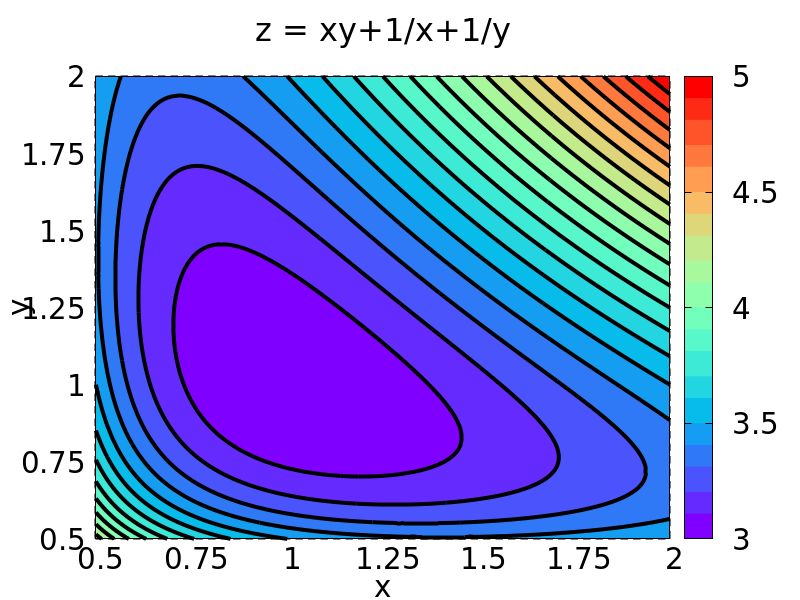
\includegraphics[width=0.65\textwidth]{./gnuplot/contour-field-extrem-values}
    \caption[Extremwertbestimmung mittels Konturlinien]{Konturlinien der zweistelligen Funktion aus Beispiel \ref{ex:CompBivarEx}. Man erkennt die Extremstelle deutlich an der geschlossenen Konturlinie.}
    \label{fig:ExCompBivarEx}
\end{figure}


% Taylor expansion, error term
\chapter{Funktionsreihen}

Eine Funktion ist eindeutig definiert durch ihre Rechenvorschrift, etwa $\sin(x)$ oder $e^x$. Doch wie können wir den Wert eines solchen Ausdrucks für eine konkrete Zahl $x$ berechnen? In der Praxis wird dies in der Regel über Näherungsverfahren getan. Ein solches Näherungsverfahren kann man mithilfe der sogenannte Taylor-Reihe gewinnen, die wir in diesem Kapitel betrachten werden. Die Taylor-Reihe stellt eine spezielle Form einer Funktionsreihe dar. Im ersten Kapitel hatten wir bereits Folgen von Zahlen betrachtet. Analog dazu ist es nun auch möglich, Folgen von Funktionen zu definieren und daraus eine Reihe zu bilden. Doch es gibt auch andere Funktionsreihen, die viele praktische Anwendungen haben. Die sogenannte Fourier-Reihe wird etwa in der Signalanalyse verwendet. Aus einem Audio-Signal, welches aufgenommen wurde als Änderung des Luftdrucks über die Zeit, kann mittels der Fourier-Analyse eine Frequenzspektrum gewonnen werden. Solch ein Frequenzspektrum lässt sich häufig wesentlich besser auf charakteristische Merkmale untersuchen, etwa um in der Spracherkennung herauszufinden, um welches Phonem oder Wort es sich handelt.

\section{Allgemeine Funktionsreihen}

Wir nähern uns dem Begriff der Funktionsreihen, indem wir zuerst endliche Reihen betrachten, also eine Reihe, welche die Summe einer endlichen Anzahl von Funktionen ist. Anschließend überlegen wir uns, was es bedeutet, eine Grenzwertbildung auszuführen. Im Gegensatz zu Zahlenreihen ist hier etwa mehr Vorsicht notwendig, da das Konvergenzverhalten anders sein kann, je nachdem, welches Argument man in die Funktionen einsetzt.

\begin{definition}{Endliche Funktionsreihe}{FunSum}
    Sei $f_n: \R \to \R, n\in\N$  eine Folge von Funktionen, welche alle den Definitionsbereich $\mathbb{D}$ besitzen. Dann versteht man unter der zugehörigen \textbf{endlichen Funktionsreihe} (Partialsummen) $F_n$ die Folge von Funktionen, welche durch Summation der ersten $n+1$-Glieder entsteht:
    $$
        F_n(x) = \sum\limits_{i=0}^n f_(x)
    $$
    Alle Glieder $F_n$ der Funktionsreihe haben den gleichen Definitionsbereich $\mathbb{D}$.
\end{definition}

Für jedes $n$ ist damit eine Funktion definiert, in die wir Argumente aus dem Definitionsbereich einsetzen können und eindeutig einen Funktionswert erhalten. Anders ausgedrückt hängt der Funktionswert also von zwei Variablen ab, dem Index $n$ und dem Argument $x$. Um nun die unendliche Reihe als Grenzwert für große $n$ definieren zu können, müssen wir zuerst den Wert für $x$ festlegen.

\begin{definition}{Grenzfunktion einer Funktionsreihe}{LimFunSum}
    Sei $F_n: \R \to \R$ eine endliche Funktionsreihe mit Definitionsbereich $\mathbb{D}$. Für jedes Argument $x$ ist dann eine Reihe gegeben, welche entweder konvergent ist oder nicht. Die Menge aller Argumente $x$, für welche diese Reihe konvergiert, nennt man das \textbf{Konvergenzintervall} $K$. Die \textbf{Grenzfunktion} ist dann die Abbildung der Argumente aus dem Definitionsbereich zu dem jeweiligen Grenzwert der Funktionsreihe für dieses Argument:
    $$
        F(x) = F_\infty(x) = \lim\limits_{n\to\infty} \sum\limits_{i=0}^n f_i(x)
    $$
\end{definition}

Man beachte dabei, dass zuerst das Argument auf einen festen Wert gesetzt wird und \emph{danach} die Grenzwertbildung ausgeführt wird.

In der praktischen Berechnung wird als Approximation statt der Grenzfunktion manchmal nur die endliche Funktionsreihe verwendet. Dadurch entsteht ein Fehler, der geringer wird, je mehr Glieder der Funktionsreihe man verwendet:

\begin{definition}{Restglied}{ErrorTerm}
    Die Differenz zwischen der Grenzfunktion $F$ und der der endlichen Funktionsreihe $F_n$ im Konvergenzintervall nennt man das Restglied $R_n$.
    $$
        R_n(x) = F(x) - F_n(x) = F(x) - \sum\limits_{i=0}^n f_(x)
    $$
    Im Grenzwert verschwindet das Restglied für alle Argumente aus dem Konvergenzintervall $\mathbb{K}$:
    $$
        \lim\limits_{n\to\infty}(x) = 0 \forall x \in \mathbb{K}
    $$
\end{definition}

Ein Beispiel für eine solche Funktionsreihe haben wir bereits im Kapitel zu Funktionen anhand der \emph{Blancmange-Funktion} gesehen. Diese stellte eine Beispiel für eine stetige, aber nirgends differenzierbare Funktion dar und ist in Abbildung \ref{fig:BlancmangeFunction} dargestellt.

\begin{example}{Funktionsreihe und Grenzfunktion}{FunSumAndLim}
    Durch $fn(x) = x^2 (1-x^2)^n$ ist für jedes $n=0,1,2,\dots$ eine Funktion im Intervall $[-1,1]$ gegeben. Durch Summation erhalten wir die Partialsummen $F_n(x) = \sum\limits_{i=0}^n x^2 (1-x^2)^i$. Die ersten Glieder lauten demnach
    \begin{alignat*}{1}
        F_0(x) &= x^2 \\
        F_1(x) &= x^2 + x^2 (1-x^2) = x^2 (2-x^2) \\
        F_2(x) &= x^2 (2-x^2) + x^2 (1-x^2)^2 = x^2 (x^4-3x^2+3)
    \end{alignat*}
    Um nun die Grenzfunktion zu erhalten, müssen wir für einen festen Wert $x$ den Grenzübergang $n \to \infty$ durchführen. Wenn wir den Funktionsterm $F_n$ genauer anschauen, stellen wir fest, dass es sich für ein festes $x$ um eine geometrische Reihe mit $p=x^2$ und $q=(1-x^2)$ handelt. Wir wissen, dass diese für $|q|=|1-x^2|<1$ konvergiert, also für $x \in [-1,1]$. Für $x=0$ ergibt sich $q=1$, doch da dann auch $p=0$ ist, konvergiert die Reihe für $x=0$ ebenfalls. Somit lautet der Konvergenzbereich der Funktionsreihe $\mathbb{K} = [-1,1]$ und der Grenzwert ergibt sich zu:
    $$
        \lim\limits_{n\to\infty} \sum\limits_{i=0}^n x^2 (1-x^2)^i = \frac{p}{1-q} = \frac{x^2}{1-(1-x^2)} = 1
    $$
    Der Graph für einige Glieder dieser Funktionsreihe findet sich in Abbildung \ref{fig:ExFunSum}. Das Restglied ist ein Maß dafür, wie nah die Partialsummen $F_n$ an der Grenzfunktion $F(x) = 1$ liegen, dies ist in Abbildung \ref{fig:ExFunErrTerm} illustriert.
\end{example}

\begin{figure}
    \centering
    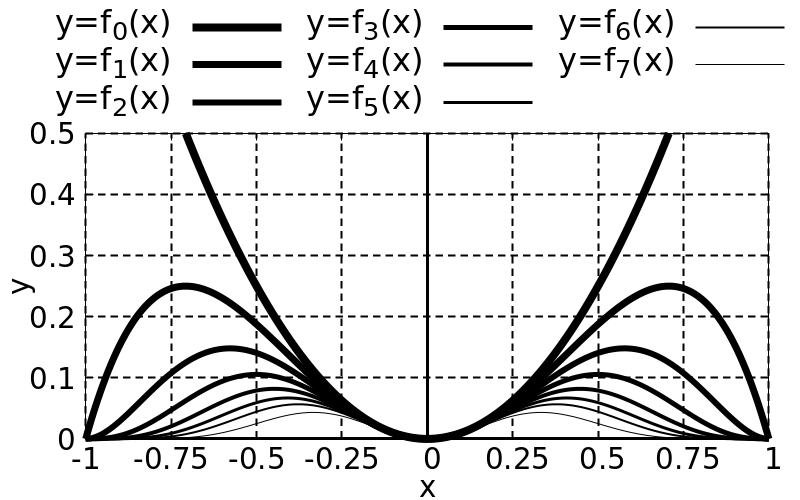
\includegraphics[width=0.45\textwidth]{./gnuplot/example-function-sum}
    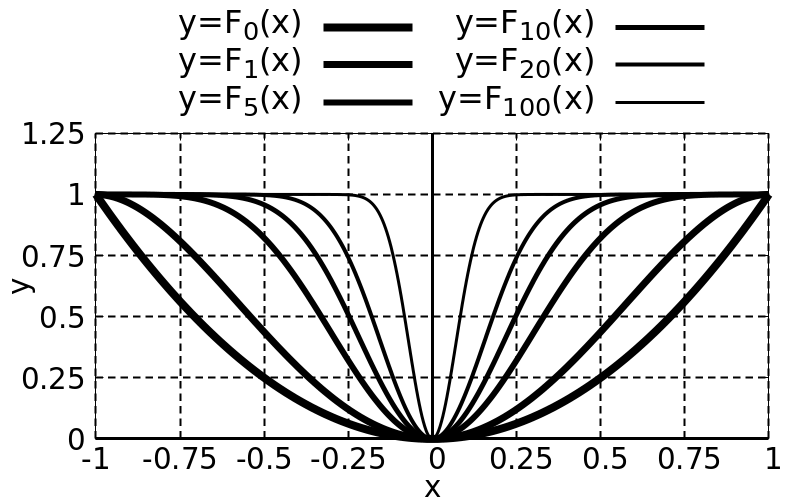
\includegraphics[width=0.45\textwidth]{./gnuplot/example-function-sum-summed}
    \caption[Einzelfunktionen und Partialsummen einer Funktionsreihe]{Beispiel einer Funktionsreihe. Links: Die Einzelfunktion $f_n$. Rechts: Die Partialsummen $F_n$.}
    \label{fig:ExFunSum}
\end{figure}

\begin{figure}
    \centering
    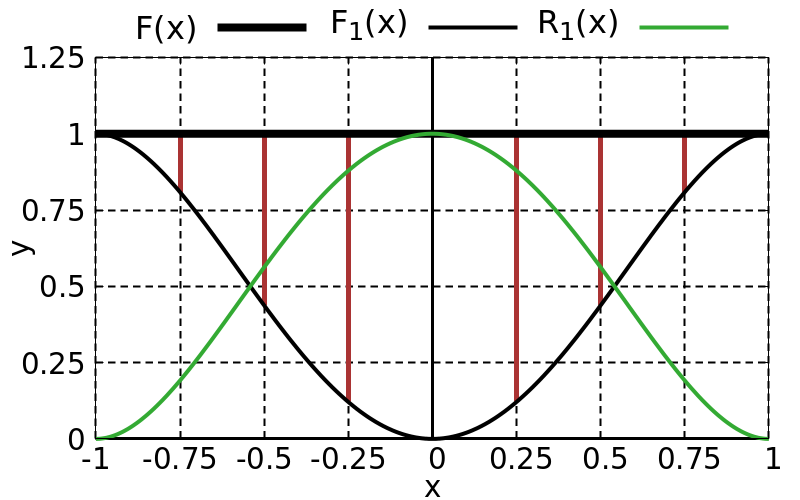
\includegraphics[width=0.65\textwidth]{./gnuplot/function-sum-error-term}
    \caption[Restglied zwischen Grenzfunktion und Partialsumme]{Graphische Bedeutung des Restglied $R_n$ als Differenz (rot) zwischen Grenzfunktion und Partialsumme.}
    \label{fig:ExFunErrTerm}
\end{figure}

Bisher haben wir nur den Grenzwert der Partialsummen für ein gegebenes $x$ betrachtet. Das Konvergenzintervall ist die Menge von Argumenten, wo dieser Grenzwert existiert. Diese Art der Konvergenz nennt man die sogenannte \textbf{punktweise Konvergenz}, da immer nur ein konkretes $x$ betrachtet wird. Jetzt kann es aber sein, dass die Partialsummen für ein bestimmtes $x$ sich dem Grenzwert nur sehr langsam nähern und für ein anderes $x$ sich sehr schnell nähern. Für viele Schlussfolgerungen im Zusammenhang mit Funktionsreihen benötigt man noch eine stärkere Art der Konvergenz. Man fordert, dass die Partialsummen für alle Argument gleich schnell, also \emph{gleichmäßig}, gegen ihren Grenzwert laufen.

\begin{definition}{Gleichmäßige Konvergenz einer Funktionsreihe}{UniformConv}
    Eine Funktionsreihe $F_n$ heißt auf einem Konvergenzintervall $\mathbb{K}$ \textbf{gleichmäßig konvergent} gegen die Grenzfunktion $F$, wenn in der Epsilon-Definition des Grenzwerts (siehe \ref{def:Convergence}) das erste Folgenglied, ab dem alle weiteren Folgenglieder einen Abstand von weniger als Epsilon vom Grenzwert haben, nur von dem gewählten Epsilon, aber nicht vom konkreten Argument $x\in\mathbb{K}$ abhängt.
    $$
        \forall \epsilon > 0 \exists n_0: \forall n > n_0, x \in \mathbb{K}: |F-F_n(x)| = |R_n(x)| < \epsilon
    $$
\end{definition}

Manchmal ist es einfacher, eine Funktion als Grenzfunktion einer Funktionsreihe darzustellen. Wie können wir von der Grenzfunktion Ableitung und Integral berechnen? Naiv könnte man jetzt auf die Idee kommen, einfach die Summanden der Funktionsreihe separat abzuleiten oder zu integrieren. Es zeigt sich aber, dass dies im allgemeinen aufgrund der Grenzwertbildung nicht möglich ist. Für gleichmäßig konvergente Funktionsreihen gilt aber die folgende Aussage:

\begin{statement}{Gliedweise Differenzierbarkeit und Integrierbarkeit}{DiffIntByParts}
    Eine auf einem Konvergenzintervall $\mathbb{K}$ gegen eine Grenzfunktion $F$ gleichmäßig konvergente Funktionsreihe $F_n$ kann gliedweise differenziert und integriert werden.
    \begin{alignat*}{1}
        \dd{}{x} F(x)      &= \lim\limits_{n\to\infty} \sum\limits_{i=0}^n \dd{}{x} f_i(x) \\
        \int F(x) \diff{x} &= \lim\limits_{n\to\infty} \sum\limits_{i=0}^n \int f_i(x) \diff{x}
    \end{alignat*}
\end{statement}

\begin{example}{Gliedweise Ableitung einer nicht gleichmäßig konvergenten Funktionsreihe}{ExNonUniformFunSum}
    Die Grenzfunktion $\sum\limits_{n=1}^\infty \frac{\sin(nx)}{n}$ existiert für alle reellen Argument $x$, beispielsweise ist $\sum\limits_{n=1}^\infty \frac{\sin(n)}{n} = \frac{\pi-1}{2}$. Leitet man nun aber jedes Glied ab, erhält man $\sum\limits_{n=1}^\infty \cos(nx)$. Diese Reihe divergiert für jedes $x$. Dies liegt daran, dass die Funktionsreihe zwar punktweise konvergent, aber nicht gleichmäßig konvergent ist.
\end{example}

\section{Potenzreihen}

Potenzreihen sind eine besondere Form von Funktionsreihen, bei denen jede Funktion $f_n$ eine Polynom vom Grad $n$ ist. Die Funktionsreihe ist damit eindeutig gegeben durch Angabe der Koeffizienten $a_n$ vor den jeweiligen Monomen. Beispielsweise ist $1+x+x^2/2+x^3/6+x^4/24 + \dots + x^n/n! + \dots$ eine solche Potenzreihe.

\begin{definition}{Potenzreihe}{PowerSum}
    Unter einer \textbf{Potenzreihe} versteht man eine Funktionsreihe, die aus Polynomen mit Koeffizienten $a_i$ gebildet wird:
    \begin{alignat*}{1}
        F_n(x) &= \sum\limits_{i=0}^n a_i x^i \\
        F(x)   &= \sum\limits_{n=0}^\infty a_n x^n
    \end{alignat*}
\end{definition}

Wir können uns nun die Frage stellen, für welche $x$ eine solchen Potenzreihe konvergiert. Offensichtlich liegt für $x=0$ Konvergenz vor, da dann alle Summanden bis auf das konstante Glied identisch $0$ sind. Um herauszufinden, für welche $x$ noch Konvergenz vorliegt, betrachten wir $x$ als Konstanten und wenden wir das Wurzelkriterium \ref{stmt:RootTest} für Reihen an. Die einzelnen Folgenglieder lauten dann $b_n = a_n \cdot x^n$.

\begin{alignat*}{1}
    q &= \lim\limits_{n\to\infty} \nroot{n}{|b_n|} \\
      &= \lim\limits_{n\to\infty} \nroot{n}{|a_n x^n|} \\
      &= \lim\limits_{n\to\infty} \nroot{n}{|a_n| \cdot |x|^n} \\
      &= \lim\limits_{n\to\infty} \nroot{n}{|a_n|} |x| \\
      &= |x| \cdot \lim\limits_{n\to\infty} \nroot{n}{|a_n|}
\end{alignat*}

Nach dem Wurzelkriterium muss nun $q<1$ gelten, damit die Reihe konvergent ist:

\begin{alignat*}{1}
             & |x| \cdot \lim\limits_{n\to\infty} \nroot{n}{|a_n|} < 1 \\
    \implies & |x| < \underbrace{\frac{1}{\lim\limits_{n\to\infty} \nroot{n}{|a_n|}}}_R
\end{alignat*}

Damit haben wir herausgefunden, dass die Potenzreihe dann konvergent ist, wenn das Argument betragsmäßig kleiner ist als der Grenzwert $R$ auf der rechten Seite. Anders ausgedrückt muss das Argument im offenen Intervall $(-R,R)$ liegen. Außerhalb dieses Intervalls, für $x > R$ beziehungsweise $x<-R$ ist $q>1$ und nach dem Wurzelkriterium die Reihe damit divergent. Am Rand dieses Intervalls ($-R,R$) ist $q=1$ und das Wurzelkriterium liefert keine Aussage, hier ist eine separate Betrachtung notwendig. Der Wert von $R$ hängt nur von den Koeffizienten $a_n$ ab und kann berechnet werden.

Die gleiche Betrachtung kann man jetzt noch einmal mit dem Quotientenkriterium \ref{stmt:RatioTest} durchführen. Wir erhalten damit die folgende Aussage.

\begin{statement}{Konvergenzradius einer Potenzreihe}
    Eine Potenzreihe $F_n(x) = \sum\limits_{i=0}^n a_i x^i$ ist für alle Argumente $|x| < R$ innerhalb des \textbf{Konvergenzradius} $R$ gleichmäßig konvergent. Der Konvergenzradius kann berechnet werden zu:
    \begin{alignat*}{1}
        1/R &= \lim\limits_{n\to\infty} \nroot{n}{|a_n|} \\
            &= \lim\limits_{n\to\infty} |\frac{a_{n+1}}{a_n}|
    \end{alignat*}
    Für $1/R=0$ ist dabei der Konvergenzradius $\infty$, die Potenzreihe konvergiert also für alle reellen Zahlen. Für $1/R=\infty$ konvergiert die Potenzreihe nirgends (bis auf $x=0$).
\end{statement}

Da die Potenzreihe im Konvergenzradius gleichmäßig konvergent ist, kann sie also gliedweise differenziert und integriert werden.

\begin{example}{Berechnung des Konvergenzradius}{ExCompConvRad}
    Wir betrachten die Potenzreihe $F_n(x) = \sum\limits_{i=0}^n \frac{1}{i!} x^i$. Die Folge der Koeffizienten lautet $a_n=\frac{1}{n!}$. Der Konvergenzradius berechnet sich über das Quotientenkriterium zu
    \begin{alignat*}{1}
        1/R &= \lim\limits_{n\to\infty} \frac{a_{n+1}}{a_n} \\
            &= \lim\limits_{n\to\infty} \frac{n!}{(n+1)!} \\
            &= \lim\limits_{n\to\infty} \frac{1}{n+1} \\
            &= 0
    \end{alignat*}
    Damit lautet der Konvergenzradius $\infty$, die Potenzreihe konvergiert also für alle reellen Argumente $x$.
\end{example}


\section{Taylor-Entwicklung}

Die Taylor-Entwicklung ist eine Rechenmethode, mit der man für eine gegebene Funktion $f$ eine Potenzreihe berechnen kann, deren Grenzfunktion der Funktion $f$ entspricht. Allerdings ist dies nicht für alle Funktionen möglich. Zur Herleitung der Taylor-Formel nehmen wir an, eine Funktion $f$ sei in eine Potenzreihe entwickelbar:

$$
    f(x) = a_0 + a_1 x + a_2 x^2 + a_3 x^3 + \dots
$$

Wie können wir dann die Koeffizienten $a_n$ bestimmen? Falls die linke und rechte Seite in der obigen Gleichung für alle Argumente $x$ im Konvergenzbereich der Potenzreihe gelten soll, muss sie speziell auch für $x=0$ gelten, dass immer zum Konvergenzradius gehört. Setzen wir $x=0$, ergibt sich:

$$
    f(0) = a_0
$$

Somit haben wir den ersten Koeffizienten $a_0 = f(0)$ der Potenzreihe bestimmt. Um den nächsten Koeffizienten zu bestimmten, leiten wir beide Seiten einmal nach $x$ ab und setzen wieder $x=0$:

\begin{alignat*}{1}
    f'(x) &= a_1 + 2 a_2 x + 3 a_3 x^2 + \dots \\
    f'(0) &= a_1
\end{alignat*}

Also lautet der zweite Koeffizient $a_1 = f'(0)$ Durch erneutes Ableiten ergeben schrittweise die weiteren Koeffizienten:

\begin{alignat*}{1}
    f''(x)  &= 2 a_2 + 6 a_3 x + \dots \\
    f'''(x) &= 6 a_3 + \dots \\
    f''(0)  &= 2 a_2 \\
    f'''(0) &= 6 a_3
\end{alignat*}

Spätestens erkennen wir ein Muster. Der Koeffizient $a_n$ ergibt sich immer als Wert der $n$-ten Ableitung von $f$ an der Stelle $0$, geteilt durch $n!$ (welches sich durch $n$-faches Ableiten des Monoms $x^n$ ergibt).

Nun sind wir bisher immer von einer Potenzreihe ausgegangen, welche um die Stelle $0$ zentriert war. Aus dem vorigen Abschnitt zu Funktionen wissen wir aber, dass wir Funktionen entlang der x-Achse um $x_0$ verschieben können, in wir das Argument durch $x \to x-x_0$ ersetzen. Damit ergibt sich die allgemeine Form der Taylor-Entwicklung:

\begin{definition}{Taylor-Reihe}{TaylorExpansion}
    Die durch eine Funktion $f$ an der \textbf{Entwicklungsstelle} $x_0$ erzeugte \textbf{Taylor-Reihe} vom \textbf{Grad n} ist gegeben durch:
    $$
        f(x) = \underbrace{\sum\limits_{i=0}^n \frac{f^{(n)}(x_0)}{n!} (x-x_0)^n}_{\text{Taylor-Reihe}} + \underbrace{R_n(x)}_{\text{Restglied}}
    $$
    Konvergiert das Restglied gegen $0$, dann hat die Taylor-Reihe $f$ als Grenzfunktion. Man sagt dann, die Funktion $f$ sei in eine Taylor-Reihe oder Potenzreihe entwickelbar.
\end{definition}

Graphisch betrachtet kann man sich die Taylor-Reihe vom Grad $n$ vorstellen als das Polynom $p_n$ vom Grad $n$, welches sich an der Stelle $x_0$ am besten an die Funktion anschmiegt. Dies ist in Abbildung \ref{fig:GraphTaylor} abgebildet. Das Polynom ist dann eine Näherung der Funktion $f$, die umso besser ist, je näher man an der Stelle $x_0$ ist. Zudem lässt sich die Näherung durch Erhöhung von $n$ verbessern. Tatsächlich ist die Taylor-Entwicklung ein Spezialfall der linearen Näherung einer Funktion für eine Tangente, denn die Taylor-Reihe vom Grad $1$ lautet

$$
    f(x) \approx f(x_0) + f'(x_0) (x-x_0)
$$

Das ist genau die Formel für die Tangente an die Funktion $f$ im Punkt $x_0$.

\begin{figure}
    \centering
    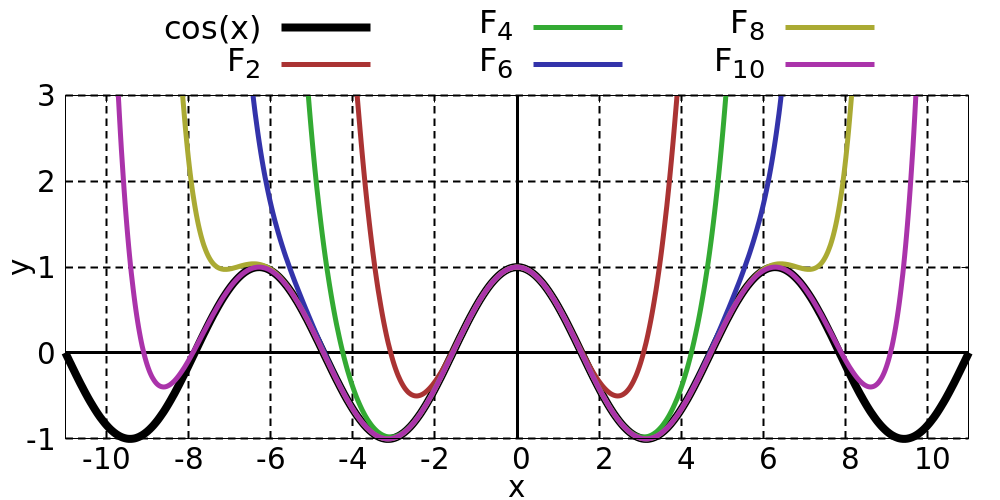
\includegraphics[width=0.65\textwidth]{./gnuplot/taylor-approximation}
    \caption[Approximation einer Funktion mittels Taylorentwicklung]{Graphische Bedeutung des der Taylorentwicklung als Approximation einer Funktion (hier: $\cos(x)$) mittels Polynomen, welche sich an der Entwicklungsstelle an die Funktion anschmiegen.}
    \label{fig:GraphTaylor}
\end{figure}

\begin{example}{Taylor-Reihe konvergiert nicht gegen Grenzfunktion}
    Wir betrachten die Taylor-Reihe, welche durch die Funktion $f(x) = e^{-\frac{1}{x^2}}$ (genauer: ihre stetige Ergänzung) an der Entwicklungsstelle $x_0=0$ erzeugt wird. Alle Ableitungen von $f$ sind von der Form $e^{-\frac{1}{x^2}} \cdot \frac{p(x)}{q(x)}$, wobei der letztere Teil eine gebrochenrationale Funktion ist. An der Entwicklungsstelle $x\to 0$ muss der Wert der $n$-ten Ableitung durch Grenzwertbildung berechnet werden. Durch mehrfache Anwendung der Regel von L'Hôpital lässt sich zeigen, dass die Exponentialfunktion im Grenzwertprozess $x\to 0$ dominiert. Damit sind alle Ableitungen an der Stelle $x_0=0$ identisch $0$. Die Taylor-Reihe lautet mithin $F_n(x) = 0$. Sie ist konvergent und hat die Grenzfunktion $F(x) = 0$. Wir haben hier ein Beispiel gefunden, wo die Taylor-Reihe existiert und konvergent ist, aber eben nicht gegen die Ausgangsfunktion $e^{-\frac{1}{x^2}}$ konvergiert.
\end{example}

\begin{example}{Berechnung der Taylor-Reihe}{CompTaylExp}
    \begin{enumerate}
        \item Alle Ableitungen von $f(x)=e^x$ sind $e^x$. An der Entwicklungsstelle $x_0=0$ ist $e^0 = 1$. Damit ist die Taylor-Reihe der Exponentialfunktion
        \begin{equation}
            e^x = 1 + x + \frac{1}{2} x^2 + \frac{1}{6}x^3 + \dots = \sum\limits_{n=0}^\infty \frac{x^n}{n!}
        \end{equation}
        Der Konvergenzradius dieser Potenzreihe ist $\infty$, wie wir bereits im Beispiel \ref{ex:ExCompConvRad} gesehen haben.
        \item Die Ableitungen von $f(x) =\sin(x)$ sind abwechselnd Sinus- und Kosinusfunktionen. Alle geraden Ableitungen sind Sinusfunktionen und daher bei $x_0=0$ identisch $0$. Für die ungeraden Ableitungen gilt $f'(x) = \cos(x)$, $f'''(x) = -\cos(x)$ und so fort. Ihre Taylor-Reihe ist damit ähnlich zu der für die Exponentialfunktion, mit dem Unterschied dass sie nur ungerade Potenzen enthält (da die Sinusfunktion eine ungerade Funktion ist) und sich die Vorzeichen abwechseln.
        \begin{equation}
            \sin(x) = x - \frac{1}{3!}x^3 + \frac{1}{5!} x^5 \mp \dots
        \end{equation}
        Diese Taylor-Reihe kann man etwa benutzen, um Wert der Sinusfunktion mit beliebiger Genauigkeit zu berechnen.
        \item Analog gilt für die Kosinusfunktion:
        \begin{equation}
            \cos(x) = 1 - \frac{1}{2}x^2 + \frac{1}{4!} x^4 \pm \dots
        \end{equation}
    \end{enumerate}
\end{example}

\begin{example}{Taylor-Reihe mit endlichen Konvergenzradius}{CompTaylorLn}
    Wir wollen die durch $f(x) = \ln(1+x)$ an der Entwicklungsstelle $x_0$ erzeugte Taylor-Reihe ermitteln. Dazu benötigen wir zuerst die Ableitungen:
    \begin{alignat*}{1}
    f^{(1)}(x) &= (1+x)^{-1} \\
    f^{(2)}(x) &= (-1) (1+x)^{-2} \\
    f^{(3)}(x) &= (-1)(-2) (1+x)^{-3} \\
    f^{(4)}(x) &= (-1)(-2)(-3) (1+x)^{-4}
    \end{alignat*}
    Allgemein gilt also $f^{(n)}(x) = (-1)^{n+1} (n-1)! (1+x)^{-n}$. Für $x_0=0$ folgt damit $f^{(n)}(0) = (-1)^{n+1} (n-1)!$ Damit erhalten wir für die Taylorreihe
    $$
        F(x) = \sum\limits_{n=0}^\infty \frac{1}{n!} (n-1)! (-1)^{n+1} x^n = \sum\limits_{n=0}^\infty \underbrace{\frac{(-1)^{n+1}}{n}}_{=a_n} x^n
    $$
    Für den Konvergenzradius dieser Potenzreihe wenden wir das Wurzelkriterium auf die Koeffizienten $a_n$ an:
    $$
        1/R = \lim\limits_{n\to\infty} \nroot{n}{|a_n|} = \lim\limits_{n\to\infty} \nroot{n}{\frac{1}{n}} = \lim\limits_{n\to\infty} 1 / \nroot{n}{n} = 1
    $$
    Der Konvergenzradius beträgt also nur $1$, die Potenzreihe konvergiert nur im Intervall $(-1,1)$ Rechts von der Stelle $x=1$ schnellt die Taylor-Reihe von der Funktion $f$ weg, unabhängig davon, wie viele Glieder man einbezieht. Dieses Verhalten ist in Abbildung \ref{fig:ExTaylorLog} dargestellt.
\end{example}

\begin{figure}
    \centering
    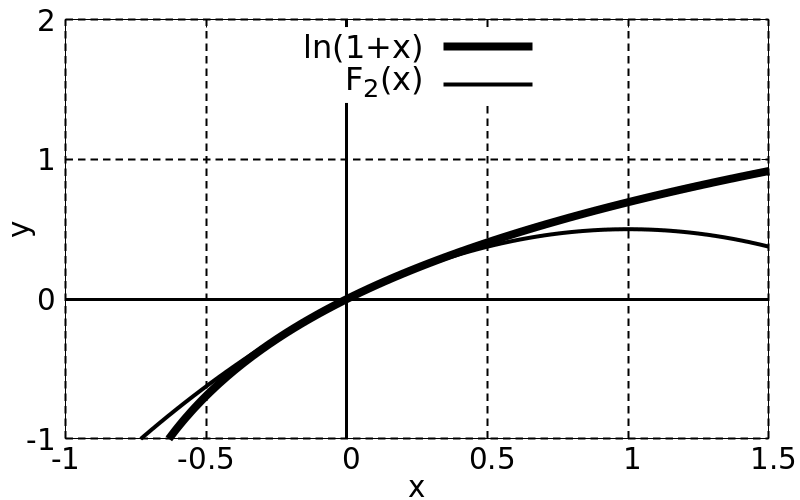
\includegraphics[width=0.45\textwidth]{./gnuplot/taylor-expansion-log-1}
    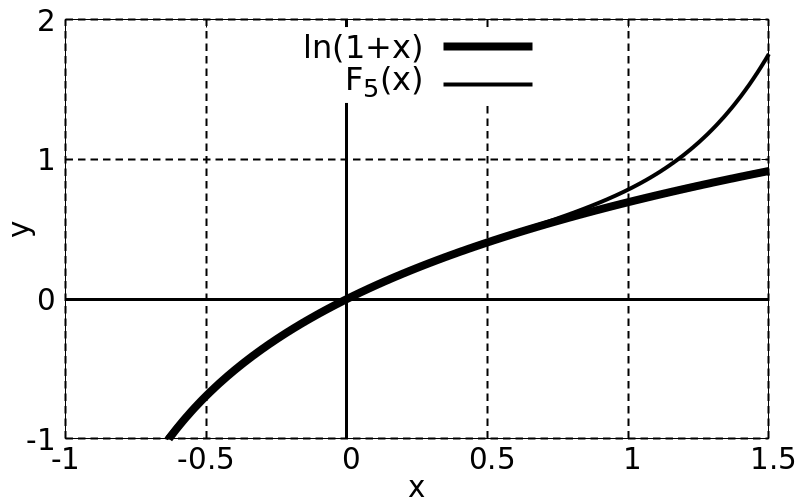
\includegraphics[width=0.45\textwidth]{./gnuplot/taylor-expansion-log-2}
    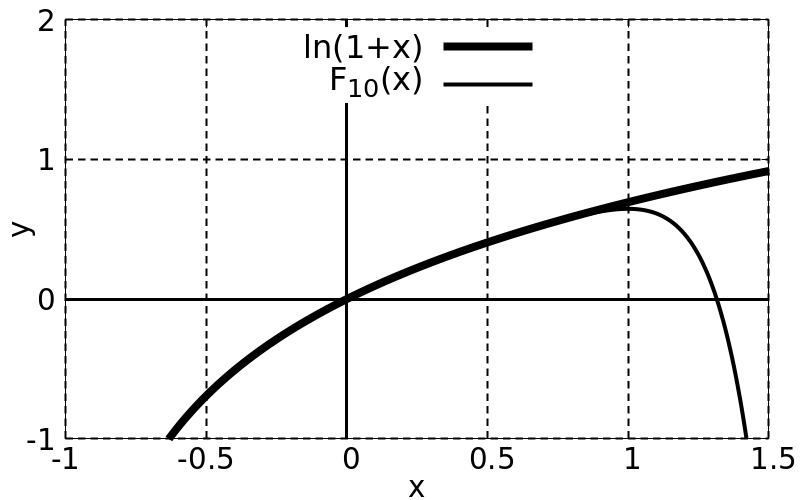
\includegraphics[width=0.45\textwidth]{./gnuplot/taylor-expansion-log-3}
    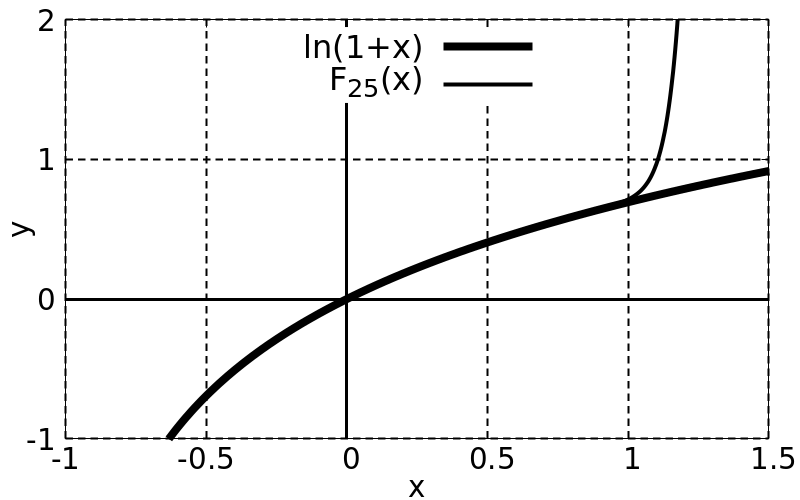
\includegraphics[width=0.45\textwidth]{./gnuplot/taylor-expansion-log-4}
    \caption[Partialsummen von Taylorreihen]{Taylor-Reihen $F_n$ der Funktion $\ln(1+x)$ für verschiedene $n$. Man erkennt, dass für $x>1$ die Reihe nicht mehr konvergiert.}
    \label{fig:ExTaylorLog}
\end{figure}

Um zu zeigen, dass eine Funktion in eine Potenzreihe entwickelbar ist, reicht es nicht aus, nur die Taylor-Reihe aufzustellen. Wir müssen zum einen zeigen, welchen Konvergenzradius die entstehende Potenzreihe hat. Doch es reicht nicht aus, dass die Potenzreihe nur konvergiert, zusätzlich müssen wir zeigen, dass die Grenzfunktion auch die Funktion $f$ ist. Dazu haben wir nachzuweisen, dass das Restglied $R_n$ für große $n$ verschwindet. Doch wie können wir das Restglied berechnen, ohne von der Grenzfunktion Gebrauch zu machen? Darüber gibt der folgende Satz Auskunft:

\begin{statement}{Restgliedform nach Lagrange}{TaylorErrPartLagrange}
    Das Restglied $R_n$ einer durch eine Funktion $f$ um die Stelle $x_0$ erzeugte Taylor-Reihe vom Grad $n$ kann dargestellt werden als:
    $$
        R_n(x) = \frac{(x-x_0)^{n+1}}{(n+1)!} f^{(n+1)}(\vartheta)
    $$
    Dabei ist $\vartheta$ eine Zahl zwischen (inklusive) der Entwicklungsstelle und dem Argument $x$.
\end{statement}

Nun macht diese Restgliedform keine Aussage darüber, welches $\vartheta$ wir denn nun nehmen sollen. Die Aussage ist lediglich, dass es ein $\vartheta$ zwischen der Entwicklungsstelle und dem Argument $x$ gibt, für die die Gleichung für das Restglied korrekt ist. $\vartheta$ hängt dabei aber in der Regel von $x$ ab. Auch wenn wir $\vartheta$ nicht genau bestimmen können, hilft diese Restgliedform dabei. Wir können zumindestens versuchen, eine Abschätzung für das Restglied zu ermitteln, um den maximalen Fehler bei einer Taylor-Reihe vom Grad $n$ zu erhalten.

Dazu betrachten wir den Betrag $|R_n|$ des Restglieds. Wir wählen $\vartheta$ im erlaubten Intervall so, dass der Wert von $f^{(n+1)}(\vartheta)$ maximal wird. Damit erhalten wir die folgende Abschätzung:

\begin{statement}{Restgliedabschätzung}{ErrTermApprox}
    Für das Restglied $R_n$ einer Taylor-Reihe vom Grad $n$ einer Funktion $f$ um die Stelle $x_0$ gilt die folgende \textbf{Restgliedabschätzung}:
    $$
        |R_n(x)| \le \frac{|x-x_0|^{n+1}}{(n+1)!} \max\limits_{\vartheta \in [x,x_0]} f^{(n+1)}(\vartheta)
    $$
\end{statement}

Die Schreibweise $\max\limits{\dots} f$ meint dabei das Maximum von $f$ innerhalb der gegebenen Grenzen des Arguments. Die Schreibweise $[x, x_0]$ meint dabei immer die Zahlen zwischen $x$ und $x_0$. Falls etwa $x=3, x_0=2$, ist mit $[3,2]$ das Intervall $[2,3]$ gemeint.

Schafft man es nun zu zeigen, dass diese Restgliedabschätzung im Grenzwert verschwindet, so tut es auch das Restglied. Ein andere Anwendungsfall ist die Fehlerabschätzung, wenn man eine Funktion durch endliche viele Glieder der Taylor-Reihe nähert.

\begin{example}{Grenzfunktion der Taylor-Reihe der Exponentialfunktion}{LimTaylorExp}
    Die durch die Exponentialfunktion erzeugte Taylor-Reihe ist überall konvergent und lautet $F_n(x) = \sum\limits_{i=0}^n \frac{x^i}{i!} + R_n(x)$. Für das Restglied gilt nach der Abschätzung:
    $$
        |R_n(x)| \le  \frac{|x|^{n+1}}{(n+1)!} \underbrace{\max\limits_{|\vartheta| < x} e^(\vartheta)}_{=e^x}
    $$
    Nach Formel \ref{eq:LimitPowerFactorial} gilt $\lim\limits_{n\to\infty} \frac{a^n}{n!} = 0$ für alle $a$, daher folgt für das Restglied $\lim\limits_{n\to\infty} R_n(x) = $. Somit konvergent die Taylor-Reihe überall gegen die Grenzfunktion $e^x$.
\end{example}

\begin{example}{Fehlerabschätzung mittels Restglied}{ErrTermApprox}
    Wir wollen den Wert $\cos(\degrees{89})$ näherungsweise bestimmen. Dazu entwickeln wir $f(x) = \cos(x)$ um die Entwicklungsstelle $\degrees{90}$ in eine Taylor-Reihe vom Grad $1$. Für die Ableitungen gilt $f'(x) = -\sin(x)$, $f''(x) = -\cos(x)$, $f'''(x) = -\sin(x)$. An der Entwicklungsstelle lauten damit die Werte $f(\degrees{90}) = 0$, $f'(\degrees{90}) = -1$, $f''(\degrees{90}) = 0$, $f'''(\degrees{90}) = 1$. Die Taylor-Reihe vom Grad $1$ ergibt sich zu:
    \begin{alignat*}{1}
        \cos(x) &= f(\degrees{90}) + f'(\degrees{90}) (x-\degrees{90}) + R_1(x) \\
                &= -(x-\degrees{90}) + R_1(x)
    \end{alignat*}
    Für $\cos(\degrees{89})$ erhalten wir so als Näherung $-\degrees{1} = \frac{\pi}{180} \approx \num{0.0174532925}\dots$. Um den Fehler zum wahren Wert von $\cos(\degrees{89})$ abzuschätzen, benutzen wir die Restgliedabschätzung. Da die zweite Ableitung an der Entwicklungsstelle $0$ ist, ist die Taylor-Reihe vom Grad $1$ mit der vom Grad $2$ identisch, wir können also statt $R_1$ auch $R_2$ verwenden. Dazu benötigen wir das Maximum von $f'''(x) = \sin(x)$ im Intervall $[\degrees{89}, \degrees{90}]$. Da die Sinusfunktion zwischen $\degrees{0}$ und $\degrees{90}$ monoton steigend ist, beträgt der Maximalwert $\sin(\degrees{90}) = 1$. Nun erhalten wir als Abschätzung für das Restglied:
    \begin{alignat*}{1}
        |R_2(\degrees{89})| &\le \frac{|-\degrees{1}|^3}{3!} \cdot 1 \\
                           &= \frac{\pi^3}{180^3 \cdot 6} \approx \num{0.000001}
    \end{alignat*}
    Wir können daher aussagen, dass unsere Schätzung bis auf die fünfte Kommastelle genau ist: $\cos(\degrees{89}) \approx  \num{0.017453} \pm \num{0.000001}$. Tatsächlich ist $\cos(\degrees{89}) = \num{0.017452406}\dots$
\end{example}

\begin{definition}{Analytische Funktion}{AnalFun}
    Eine Funktion, die im gesamten Definitionsbereich als Taylor-Reihe dargestellt werden kann, heißt \textbf{analytische Funktion}.
\end{definition}

Bemerkenswert an der Taylor-Entwicklung ist, dass diese nur von dem Wert der Funktion und ihren Ableitung an der Entwicklungsstelle abhängt. Nur Werte nahe der Entwickklungsstelle spielen eine Rolle, da diese für die Ableitung (Grenzwert des Differenzenquotienten) bedeutsam sind. Werte "weit weg" von der Entwicklungsstelle sind irrelevant. Jetzt kann "weit weg" aber beliebig nahe sein. Sobald die Werte einer analytischen Funktion in einem beliebig kleinen offenen Intervall um die Entwicklungsstelle bekannt sind, können wir die Taylorreihe eindeutig bestimmen. Und in die Taylor-Reihe ist es und möglich, die Werte der Funktion an jeder anderen Stelle $x$ zu berechnen. In anderen Worten bedeutet dass, das eine analytische Funktion eindeutig durch ihre Werte in einem kleinen (offenen) Intervall definiert ist. Die sogenannte analytische Fortsetzung wird in der Mathematik benutzt, um eine Funktion für Werte zu definieren, die sich nicht aus der ursprünglichen Definition oder Rechenvorschrift ergeben.

Wir können noch eine weitere interessante Schlussfolgerung daraus ziehen. Manchmal benötigt man in der Mathematik Funktionen, die nur in einem beschränkten Bereich (etwa zwischen $0$ und $1$) einen Wert ungleich $0$ haben und für alle anderen Werte identisch $0$ sind. Eine Formel für eine solche Funktion anzugeben ist deshalb nicht ganz so leicht, da es sich nicht um eine analytische Funktion handeln kann. Denn die Funktion ist außerhalb identisch $0$, wodurch ihre Taylor-Reihe eindeutig bestimmt ist. Aber die Taylor-Reihe ist somit $0$ und damit muss die gesamte Funktion überall $0$ sein.

\begin{example}{Ableitung der Exponentialfunktion}{ExDiffExpFunTaylor}
    Die Exponentialfunktion hat die Potenzreihendarstellung $e^x=\sum\limits_{n=0}^\infty \frac{x^n}{n!}$. Durch gliedweises Ableiten erhalten wir $\dd{}{x} e^x = \sum\limits_{n=1}^\infty n \cdot \frac{x^{n-1}}{n!}$. Mittels Kürzen erhalten wir $\sum\limits_{n=1}^\infty \cdot \frac{x^{n-1}}{(n-1)!}$. Verschieben wir nun noch den Laufindex $i = n-1$, so ergibt sich $\sum\limits_{i=0}^\infty \cdot \frac{x^i}{i!}$. Dies ist aber nichts anderes als die Potenzreihe der Exponentialfunktion. Somit haben wir uns vergewissert, dass die Ableitung der Exponentialfunktion identisch zu sich selber ist: $\dd{}{x}e^x = e^x$. (Hinweis: Dies ist in dem Sinne kein Beweis, solange wir die Potenzreihe durch Berechnung der Taylor-Reihe ermitteln, wofür wir die Ableitung der Exponentialfunktion benötigen.)
\end{example}

Abschließend in diesem Abschnitt sei noch angemerkt, dass man auch für mehrstellige Funktionen $f:\R^n\to \R$ eine Taylor-Reihe aufstellen kann. Diese lässt sich mithilfe des Nabla-Operator und der Potenzreihendarstellung $e^{\star} = 1 + \star + \frac{1}{2} \star^2 + \dots$ kurz und bündig schreiben als:

$$
    f(\vec{r}+\vec{\Delta r}) = e^{\vec{\nabla} \vec{\Delta r}} f(\vec{r})
$$

\section{Fourier-Entwicklung}

Eine weitere bedeutende Funktionsreihe ist die sogenannte \emph{Fourier-Reihe}. Hat man mit einem Mikrofon ein Audiosignal aufgenommen, ist dieses durch den Wert des Luftdrucks zu jedem Zeitpunkt gegeben. Von Interesse ist aber oft, welche Frequenzen in dem Audio-Signal mit welcher Amplitude enthalten sind. Etwa erzeugt ein Musikinstrument einen Ton, welcher eine Überlagerung einer harmonischen Grundschwindung mit einem oder mehreren Obertönen ist. Diese einzelnen Töne sind sinus- und kosinusförmige Schwingungen. Mathematisch kann man daher die Frequenzen eines Signals erhalten, indem man versucht, es als Funktionsreihe darzustellen, bei der die einzelnen Funktion Sinus- und Kosinusfunktionen sind.

\begin{definition}{Trigonometrische Reihe}{TriSum}
    Eine \textbf{trigonometrische Reihe} ist eine Funktionsreihe, deren Einzelfunktionen Sinus- und Kosinusfunktionen sind:
    $$
        F_n(x) = \sum\limits_{i=0}^n a_i \cos(ix) + b_i \sin(ix)
    $$
\end{definition}

Man beachte, dass alle Einzelfunktion $2\pi$ als Periode (nicht Fundamentalperiode) haben. Damit hat auch die Grenzfunktion, falls sie denn existiert, die Periode $2\pi$. Wenn wir eine Funktion $f$ als trigonometrische Reihe darstellen wollen, ist dies daher zuerst einmal nur sinnvoll, wenn $f$ auch die Periode $2\pi$ hat. Die Koeffizienten $a_1$ und $b_1$ beschreiben dann die Amplitude der Grundfrequenz $f=\frac{1}{2\pi}$. Die nächsten beiden Koeffizienten $a_2, b_2$ dann die Amplitude der ersten Oberfrequenz $2f$, $a_3, b_3$ die Amplituden für $3f$, \dots.

Für die Herleitung gehen wir zuerst einmal davon aus, dass $f$ die Periode $T=2\pi$ habe. Analog zur Taylor-Entwicklung können wir uns nun fragen, wie wir für eine konkrete Funktion $f$ die Koeffizienten $a_n$ und $b_n$ bestimmen können. Wir stellen fest, dass $b_0$ irrelevant ist, da $\sin(nx)$ für $n=0$ immer gleich $0$ ist. Als nächstes multiplizieren wir beide Seiten der Gleichung mit $\cos(x)$ und bilden das Integral von $0$ bis $2\pi$ (das $\diff{x}$ ist hier zu Kürze ausgelassen)

\begin{alignat*}{1}
    f(x)                              &= a_0 + a_1 \cos x + a_2 \cos 2x + \dots + b_1 \sin x + b_1 \sin 2x + \dots \\
    \int\limits_0^{2\pi} \cos(x) f(x) &= a_0 \int\limits_0^{2\pi} \cos(x) \cos 0x           + a_1 \int\limits_0^{2\pi} \cos x \cos x + a_2 \int\limits_0^{2\pi} \cos x \cos 2x + \dots \\
                                      &\phantom{{}= a_0 \int\limits_0^{2\pi} \cos(x) \cos 0x} + b_1 \int\limits_0^{2\pi} \cos x \sin x + b_1 \int\limits_0^{2\pi} \cos x \sin 2x + \dots
\end{alignat*}

Durch partielle Integration lassen sich diese Integrale berechnen. Allgemein gilt für $m,n\in\N$:

\begin{alignat*}{1}
    \int\limits_0^{2\pi} \cos(mx) \cos(nx) \diff{x} &= \begin{cases} \pi & , n = m > 0 \\ 2 \pi &, n = m = 0 \\ 0 &, \text{sonst} \end{cases} \\
    \int\limits_0^{2\pi} \sin(mx) \sin(nx) \diff{x} &= \begin{cases} \pi & , n = m > 0 \\ 0 &, \text{sonst} \end{cases} \\
    \int\limits_0^{2\pi} \sin(mx) \cos(nx) \diff{x} &= 0
\end{alignat*}

Damit erhalten wir für den Koeffizienten $a_1$:

$$
    \int\limits_0^{2\pi} \cos(x) f(x) \diff{x} = a_1 \pi
$$

Analog dazu können wir auch mit $\cos(0x)$, $\cos(2x)$, $\cos(3x)$, \dots sowie $\sin(x), \sin(2x), \dots$ multiplizieren und erhalten die anderen Koeffizienten:

\begin{alignat*}{1}
    a_0 &= \frac{1}{2\pi} \int\limits_0^{2\pi} f(x) \diff{x} \\
    a_n &= \frac{1}{\pi} \int\limits_0^{2\pi} f(x) \cos(nx) \diff{x} \\
    b_n &= \frac{1}{\pi} \int\limits_0^{2\pi} f(x) \sin(nx) \diff{x}
\end{alignat*}

Nun müssen wir noch berücksichtigen, dass wir bisher davon ausgegangen waren, dass $f$ die Periode $2\pi$ hätte. Ist dies nicht der Fall und besitzt $f$ eine andere Periode $T$, können wir die obigen Formeln modifizieren, indem wir entlang der Abszisse entsprechend skalieren. Wir erhalten damit die Fourier-Reihe:

\begin{definition}{Fourier-Reihe}{FourierExpansion}
    Die durch eine Funktion $f$ mit der Periode $T$ erzeugte \textbf{Fourier-Reihe} ist gegeben durch:
    $$
        f(x) = \underbrace{\sum\limits_{i=0}^n a_i \cos(\frac{2\pi}{T}ix) + b_n \sin(\frac{2\pi}{T}ix)}_{\text{Fourier-Reihe}} + \underbrace{R_n(x)}_{\text{Restglied}}
    $$
    Die Koeffizienten $a_n$ und $b_n$ lauten dabei:
    \begin{alignat*}{1}
        a_0 &= \frac{1}{T} \int\limits_0^{T} f(x) \diff{x} \\
        a_n &= \frac{2}{T} \int\limits_0^{T} f(x) \cos(\frac{2\pi}{T}nx) \diff{x} \\
        b_n &= \frac{2}{T} \int\limits_0^{T} f(x) \sin(\frac{2\pi}{T}nx) \diff{x}
    \end{alignat*}
\end{definition}

Mithilfe dieser Fourier-Reihe können wir ein Signal nehmen und es in die Frequenzdomäne überführen. Die Koeffizienten $a_n$ und $b_n$ entsprechen dann der Amplitude der Frequenz $f_n = \frac{1}{nT}$. Sie sind ein Maß dafür, wie viel von der jeweiligen Frequenz im Signal enthalten ist. Zur Berechnung müssen wir die entsprechenden Integral berechnen, wie im Beispiel \ref{ex:ExFourUnitStep} gezeigt wird.

\begin{example}{Fourier-Reihe der Einheitsschrittfunktion}{ExFourUnitStep}
    Die Einheitsschritt Funktion ist gegeben durch $f(x) = 0$ für $x \in [0, 0.5)$, $f(x) = 1$ für $x \in [0.5, 1)$ und $f(x+k) = f(x)$ mit $k=\pm 1,\pm 2, \pm 3, \dots$. Die Periode ist $T=1$. Wir beginnen mit dem Fourier-Koeffzienten $a_0$:
    $$
        a_0 = \frac{1}{T} \int\limits_0^{T} f(x) \diff{x} = \frac{1}{T} \int\limits_{1/2}^{1} 1 \diff{x} = \frac{1}{2}
    $$
    Das Integral wird nur für $1/2$ bis $1$ berechnet, da $f$ im anderen Teil identisch $0$ ist. Für die Koeffizienten $a_n$ folgt:
    \begin{alignat*}{1}
        a_n &= \frac{2}{1} \int\limits_{1/2}^{1} \cos(2\pi n x) \diff{x} \\
            &= 2 \frac{1}{2 \pi n} \left[ \sin(2\pi n x) \right]_{x=1/2}^1 \\
            &= \frac{1}{\pi n} \cdot 0 = 0
    \end{alignat*}
    Und für die Koeffizienten $b_n$:
    \begin{alignat*}{1}
        b_n &= \frac{2}{1} \int\limits_{1/2}^{1} \sin(2\pi n x) \diff{x} \\
            &= 2 \frac{1}{2 \pi n} \left[ -\cos(2\pi n x) \right]_{x=1/2}^1 \\
            &= \frac{1}{\pi n} \cdot (-1+(-1)^n) \\
            &= \begin{cases} -\frac{2}{\pi n} & , n \text{ ungerade} \\ 0 &, n \text{ gerade} \end{cases}
    \end{alignat*}
    Folglich lässt sich die Einheitsschrittfunktion aus Abbildung \ref{fig:ExUnitStepFourier} schreiben als:
    $$
        f(x) = \frac{1}{2} - \frac{2}{\pi} \sum\limits_{n=1}^\infty \frac{1}{2n-1} \sin(2\pi (2n-1) x)
    $$
    Man beachte, dass die Einheitsschrittfunktion nicht stetig ist, die Fourier-Reihe nähert sich trotzdem der Funktion an.
\end{example}

\begin{figure}
    \centering
    \includegraphics[width=0.45\textwidth]{./gnuplot/fourier-transform-step-1}
    \includegraphics[width=0.45\textwidth]{./gnuplot/fourier-transform-step-2}
    \includegraphics[width=0.45\textwidth]{./gnuplot/fourier-transform-step-3}
    \includegraphics[width=0.45\textwidth]{./gnuplot/fourier-transform-step-4}
    \caption{Erste Glieder der Fourier-Rehe einer Einheitsschrittfunktion}
    \label{fig:ExUnitStepFourier}
\end{figure}

Nun ist es im Gegensatz zu Potenzreihen nicht so, dass die trigonometrische Reihe immer gleichmäßig konvergiert. Es gilt allerdings, dass wenn die Fourier-Reihe einer $f$ gleichmäßig konvergent ist, dass sie dann auch $f$ als Grenzfunktion hat, das Restglied also verschwindet. Diese Bedingung ist eine hinreichende, jedoch keine notwendige. Eine für die Praxis meist bessere Bedingung gibt der folgende Satz:

\begin{statement}{Dirichletsche Bedingung}{DirchCondFourier}
    Sei $f$ ein beschränkte, periodische Funktion mit der Periode $T$ und definiert im Intervall $[0,T)$. Wenn sich das Intervall $(0,2\pi)$ zerlegen lässt in endlich viele Teilintervalle, in derem jeden die Funktion $f$ stetig und monoton ist, so konvergiert die durch die Funktion $f$ erzeugte Fourier-Reihe für jede Stetigkeitsstelle $x_0$ gegen den Funktionswert $f(x_0)$ und für jede Sprungstelle $x_S$ gegen das arithmetische Mittel aus links- und rechtsseitigen Grenzwert $\frac{1}{2} \cdot \left(\lim\limits_{x\to x_S^-} + \lim\limits_{x\to x_S^+}\right)$.
\end{statement}

Das heißt also, dass wir im Gegensatz zur Taylor-Entwicklung mit der Fourier-Entwicklung auch unstetige Funktionen darstellen können. Beispielsweise werden in der Tontechnik und Elektrotechnik Rechteckimpulse verwendet, der dadurch gekennzeichnet ist, dass er innerhalb eines Intervalls den Wert $1$ und außerhalb davon den Wert $0$ besitzt. An der Grenze liegt also eine Sprungstelle vor. Dennoch kann man eine Fourier-Entwicklung durchführen und die Frequenzen des Rechteckimpulses ermitteln. In Abbildung \ref{fig:ExFourierDirichlet} ist dies am Beispiel einer Funktion mit mehreren Unstetigkeitsstellen dargestellt.

\begin{figure}
    \centering
    \includegraphics[width=0.65\textwidth]{./gnuplot/fourier-dirichlet}
    \caption[Fourier-Reihe einer unstetigen Funktion]{Unstetige Funktion und die Grenzfunktion der durch sie erzeugten Fourier-Reihe. Beide stimmen in allen Stetigkeitsstellen überein. An den Unstetigkeitsstellen wird das arithmetische Mittel zwischen links- und rechtsseitigen Grenzwert angenommen.}
    \label{fig:ExFourierDirichlet}
\end{figure}

\begin{example}{Grenzfunktion der Fourier-Reihe der Einheitsschrittfunktion}{ExUnitStepLim}
    Die Einheitsschrittfunktion aus Beispiel \ref{ex:ExFourUnitStep} lässt sich durch die Fourier-Reihe $\frac{1}{2} - \frac{2}{\pi} \sum\limits_{n=1}^\infty \frac{1}{2n-1} \sin(2\pi (2n-1) x)$ darstellen. Nun lässt sich die Einheitsschrittfunktion in die zwei Teilintervalle $(0, 0.5)$ und $(0,5, 1)$ zerlegen, in denen beiden sie stetig und monoton ist. Daher konvergiert sie dort gegen den Grenzfunktion, also die Einheitsschrittfunktion. Für $x=0,0.5,1.0,\dots$ konvergiert sich den Mittelwert aus links- und rechtsseitigen Grenzwert, also gegen $\frac{1}{2} (0+1) = \frac{1}{2}$.
\end{example}

Zwei Bemerkungen noch zu praktischen Anwendungen. Zum einen können wir nicht nur eine Funktion auf ihre Frequenzen analysieren, sondern auch eine Funktion aus gegebenen Frequenzen zusammensetzen. Dies nennt man die sogenannten \emph{harmonische Synthese}. Diese wurde etwa früher genutzt, um gesprochene Sprache und Instrumententöne unter Anderem aus einfachen Sinus- und Kosinusschwingungen zusammenzusetzen. Da solche Signale aber komplexer sind, also aus mehr als einigen wenigen Frequenzen bestehen, lässt die Qualität dabei auch zu wünschen übrig. Daher werden heute meist aufgenommene Samples modifiziert und zusammengesetzt.

Zum Zweiten ist es so, dass man in der Praxis ein Signal nicht für jeden beliebigen Zeitpunkt kennt, um das Integral für die Koeffizienten der Fourier-Reihe bestimmten zu können. Aus dem Kapitel zur Infinitesimalrechnung wissen wir aber, dass das unbestimmte Integral als Grenzwert von Flächeninhaltssummen definiert war. Wenn wir das Signal beziehungsweise die Funktion nur an einer endlichen abzählbaren Menge von Stellen kennen, können wir die Fourierkoeffizienten mit einer endlichen Summenbildung statt dem Integral annähern.

\begin{definition}{Diskrete Fourier-Transformation}{DiscFourTrans}
    Eine Funktion $f$ mit der Periode $T$ sei im Intervall $[0, T]$ an den $2m$ Stellen $x_i = \frac{T}{2m} i$ ($0\le i < 2m-1$) gegeben mit den Funktionswerten $y_i$. Dann ist die die diskrete \textbf{Fourier-Transformation} definiert durch
    $$
        F[f](x) = a_0 + \sum\limits_{i=1}^m a_i \cos(\frac{2\pi}{T}ix) + b_i \sin(\frac{2\pi}{T}ix)
    $$
    Die Fourier-Koeffizienten berechnen sich dabei zu:
    \begin{alignat*}{1}
        a_0 &= \frac{1}{2m} \sum\limits_{i=0}^{2m-1} y_i  \\
        a_n &= \frac{1}{m} \sum\limits_{i=0}^{2m-1} y_i \cos(\frac{\pi}{m} ni) \\
        b_n &= \frac{1}{m} \sum\limits_{i=0}^{2m-1} y_i \sin(\frac{\pi}{m} ni) \\
        a_m &= \frac{1}{2m} \sum\limits_{i=0}^{2m-1} y_i \cos(i\pi)
    \end{alignat*}
\end{definition}

Ein Beispiel für das diskrete Frequenz-Spektrum eines Audio-Signals findet sich im Anhang in Abbildung \ref{fig:SpeechFreq}.

Bis hierher haben wir immer nur diskrete Frequenzen (Grundfrequenz $\frac{1}{T}$ und Vielfache) betrachtet. Abschließend sei noch angemerkt, dass es für einen kontinuierlichen Frequenz-Bereich noch die die sogenannte Fourier-Transformation gibt, welche einer Funktion ihre Fourier-Transformierte zuordnet:

$$
    \mathcal{F}[f(t)](\omega) = \frac{1}{\sqrt{2\pi}} \int\limits_{-\infty}^\infty f(t) e^{-j \omega t} \diff{t}
$$

% Differential equations, definitions, simple solving techniques
\chapter{Differntialgleichungen}

Definition von DGL

Eigenschaften von DGL

Einfach Lösungsmethoden
  Direkte Integration
  Trennung der Variables
  Variation der Konstanten
  Struktur der Lsg. von lin. DGL
  Charakt. Gleichung für homog. Anteil
  Ansatz für inhomog. Anteil


\appendix

\chapter{Ergänzende Abbildungen}

\begin{figure}[H]
    \label{fig:ContourComplexFun}
    \centering
    \includegraphics[width=0.95\textwidth]{./gnuplot/example-contour-field-complex}
    \caption{Konturlinien mit farbiger Hervorhebung für eine Funktion. Jede Farbe entspricht einem Funktionswert, wie er in der Legende rechts zu sehen ist.}
\end{figure}

\begin{figure}[H]
    \label{fig:UniLogScale}
    \centering
    \includegraphics[width=0.95\textwidth]{./img/universe-log-scale}
    \caption{Künstlerische Darstellung des beobachtbaren Universums in logarithmischer Skalierung und Zentrierung auf das Sonnensystem. Abgebildet sind die inneren und äußeren Planeten des Sonnensystems, der Kuipergürtel, die Oortsche Wolke, Alpha Centauri, Perseusarm, die Milchstraße, der Andromedanebel, Nachbargalaxien, das Kosmische Netz, die Kosmische Hintergrundstrahlung und der Plasmazustand kurz nach dem Urknall. Quelle: \href{https://commons.wikimedia.org/wiki/User:Unmismoobjetivo}{Pablo Carlos Budassi}, \href{https://commons.wikimedia.org/wiki/File:Observable_universe_logarithmic_illustration.png}{wikimedia}}
\end{figure}


\tcblistof[\chapter]{definition}{Liste der Definitionen}

\tcblistof[\chapter]{statement}{Liste der Aussagen}

\tcblistof[\chapter]{example}{Liste der Beispiele}

\clearpage

\listoffigures

\backmatter

%%% BIBLIOGRAPHY
%%% -------------------------------------------------------------

% \bibliographystyle{utphysics}
% \bibliography{ref}

\end{document}
